\documentclass[fontsize=14pt,a4paper,DIV=14,open=any]{scrreprt}

%%%%%%%% CREATE DOCUMENT STRUCTURE %%%%%%%%
%% Language and font encodings
\usepackage[english]{babel}
\usepackage[utf8x]{inputenc}
\usepackage[T1]{fontenc}
\usepackage{csquotes}  % required by biblatex when babel is loaded

%% Page margins
\usepackage[top=2cm,bottom=2cm,left=1.5cm,right=1.5cm]{geometry}
\setlength{\footskip}{20pt}  % push footer up so page number isn't clipped

%% Useful packages
\usepackage{lmodern}
\usepackage{amsmath}
\usepackage{graphicx}
\graphicspath{{images/}}
\usepackage{caption}
\usepackage{xcolor}
\usepackage{scrhack}  % must come before float/listings to patch KOMA incompatibilities
\usepackage{float}
\usepackage{listings}
\definecolor{darkgreen}{rgb}{0.0, 0.4, 0.0}
\definecolor{codegreen}{rgb}{0,0.6,0}
\definecolor{codegray}{rgb}{0.5,0.5,0.5}
\definecolor{codepurple}{rgb}{0.58,0,0.82}
\definecolor{backcolour}{rgb}{0.95,0.95,0.92}
\lstset{ 
    backgroundcolor=\color{backcolour},   
    commentstyle=\color{codegreen},
    keywordstyle=\color{magenta},
    numberstyle=\tiny\color{codegray},
    stringstyle=\color{codepurple},
    basicstyle=\ttfamily\footnotesize,
    breakatwhitespace=false,         
    breaklines=true,                 
    captionpos=b,                    
    keepspaces=true,                 
    numbers=left,                    
    numbersep=5pt,                  
    showspaces=false,                
    showstringspaces=false,
    showtabs=false,                  
    tabsize=2
}
\usepackage[backend=biber, style=ieee]{biblatex}
\addbibresource{references.bib}
%% hyperref loaded last
\usepackage[colorlinks=true, urlcolor=blue, linkcolor=black, citecolor=blue]{hyperref}

%% KOMA-Script font settings
\setkomafont{chapter}{\huge\bfseries}
\setkomafont{section}{\Large\bfseries}
\setkomafont{subsection}{\large\bfseries}

%% Abstract heading style
\renewcommand{\abstractname}{Abstract}
\renewenvironment{abstract}{%
  \clearpage\null\vfill
  \begin{center}
    {\Huge\bfseries\abstractname}
  \end{center}
  \vspace{1em}
  \par\noindent\ignorespaces
}{\par\vfill\null\clearpage}

%%%%%%%% DOCUMENT %%%%%%%%
\begin{document}
\pagenumbering{arabic}

%%%% Title Page
\begin{titlepage}
    \newcommand{\HRule}{\rule{\linewidth}{0.5mm}}
    \centering
    \vspace*{3cm}
    % University
    \textsc{\LARGE Universita di Pisa}\\[1cm]
    
\includegraphics[width=0.2\textwidth]{unipi_logo.png}\\[1cm]
    % Document info
    \textsc{\Large Master's Thesis}\\[0.2cm]
    \textsc{\large Supervised by: Professor Alessio Giorgetti}\\
    \HRule\\[0.3cm]
    {\huge\bfseries Thesis Title}\\
    \HRule\\[5cm]
    \emph{By: ASM Chafiullah Bhuiyan}\\
    Computer Science and Networking\\[0.2cm]
    \emph{\textbf{Academic Year: 2025--2026}}
    \vfill
\end{titlepage}
%%% Acknowledgement
\section*{\begin{center}
      Acknowledgement
  \end{center}}
First and foremost, I would like to express my deepest gratitude to my primary supervisor, Professor Alessio Giorgetti. I am incredibly thankful for his unwavering support, his willingness to share his resources, and for granting me welcoming access to his office. His generous investment of valuable time and expertise was instrumental in allowing me to complete this extensive and complex project within the given timeframe. Furthermore, I am deeply appreciative of his provision of dedicated hardware resources, which afforded me endless opportunities to conduct rigorous testing and successfully validate my work.

\vspace{0.4cm}
Finally, words cannot adequately express my profound gratitude to my family for their immense sacrifices during my time studying abroad. I owe a special and heartfelt thank you to my children, who have had to navigate a significant part of their childhood missing their father. Your love, patience, understanding, and resilience have been my greatest source of strength and motivation throughout this journey. This thesis is as much yours as it is mine.

%%% Abstract
\begin{abstract}
    \begin{center}
        \textsc{\large Thesis Title}\\[0.2cm]
        \textsc{\large Master's in Computer Science and Networking}\\[1cm]
    \end{center}
    The provisioning of light-paths in flexible-grid optical networks has significantly enhanced spectrum utilization; however, the integration of topologies featuring multiple parallel links between optical devices introduces profound computational complexities in Routing and Spectrum Allocation (RSA). Specifically, when multiple transponders (muxponders) interface with the exact same degree of Reconfigurable Optical Add-Drop Multiplexer (ROADM) devices, the permutation of viable routing options increases exponentially. This geometric expansion renders standard path computation mechanisms excessively heavy and inefficient for traditional Software-Defined Networking (SDN) controllers. This routing challenge is further compounded by the stringent constraints of spectrum continuity and contiguity under the ITU-T G.694.1 standard, which dictates a 12.5 GHz minimum slot width and a high-resolution 6.25 GHz slot granularity. Because optical signals directed to the same ROADM degree cannot reuse identical frequencies without severe interference, the controller is burdened with the computationally intensive task of continuously verifying the availability of every individual 6.25 GHz slot across all potential parallel routes. To overcome these dual bottlenecks of path scalability and high-resolution spectrum mapping, this thesis introduces the ParallelOpticalController, a novel microservice engineered directly into the \texttt{TeraFlowSDN} ecosystem. Leveraging the \texttt{networkX} library for advanced topological graph modeling, the proposed architecture natively supports multi-directed graphs with parallel edges. This enables the highly efficient execution of Dijkstra's algorithm to compute the optimal shortest path, while concurrently discovering and suggesting exhaustive alternative path combinations to maximize network utilization. Furthermore, to resolve the heavy spectrum calculation overhead, the controller employs an innovative bitwise mapping algorithm that performs mathematical intersections of available flex-grid slots across sequential hops, drastically reducing the time required to identify contiguous spectrum blocks. Finally, these backend computational advancements are fully integrated with a dynamic graphical WebUI that visualizes the complex parallel-link topology, endpoint interfaces, and real-time spectrum allocations, thereby offering a highly scalable, end-to-end framework for next-generation optical network management.
\end{abstract}
%%% Contents
\tableofcontents
\listoffigures
\listoftables
% additional file for Chapter 1
\chapter{Introduction}
\section{Overview}
The unprecedented surge in global data traffic, driven largely by the widespread deployment of 5G cellular networks and Fiber-to-the-Home (FTTH) access architectures, has fundamentally reshaped the telecommunications landscape. To satisfy this monumental and continuous demand without incurring the prohibitive costs of laying new physical fiber, network operators are compelled to maximize the transmission capacity of existing optical resources. This is primarily achieved by aggregating multiple communication channels into a single optical fiber using Wavelength Division Multiplexing (WDM) and, more specifically, Dense Wavelength Division Multiplexing (DWDM), which increases fiber efficiency by transmitting independent signals at different wavelengths.
\begin{figure}[htbp]
    \centering
    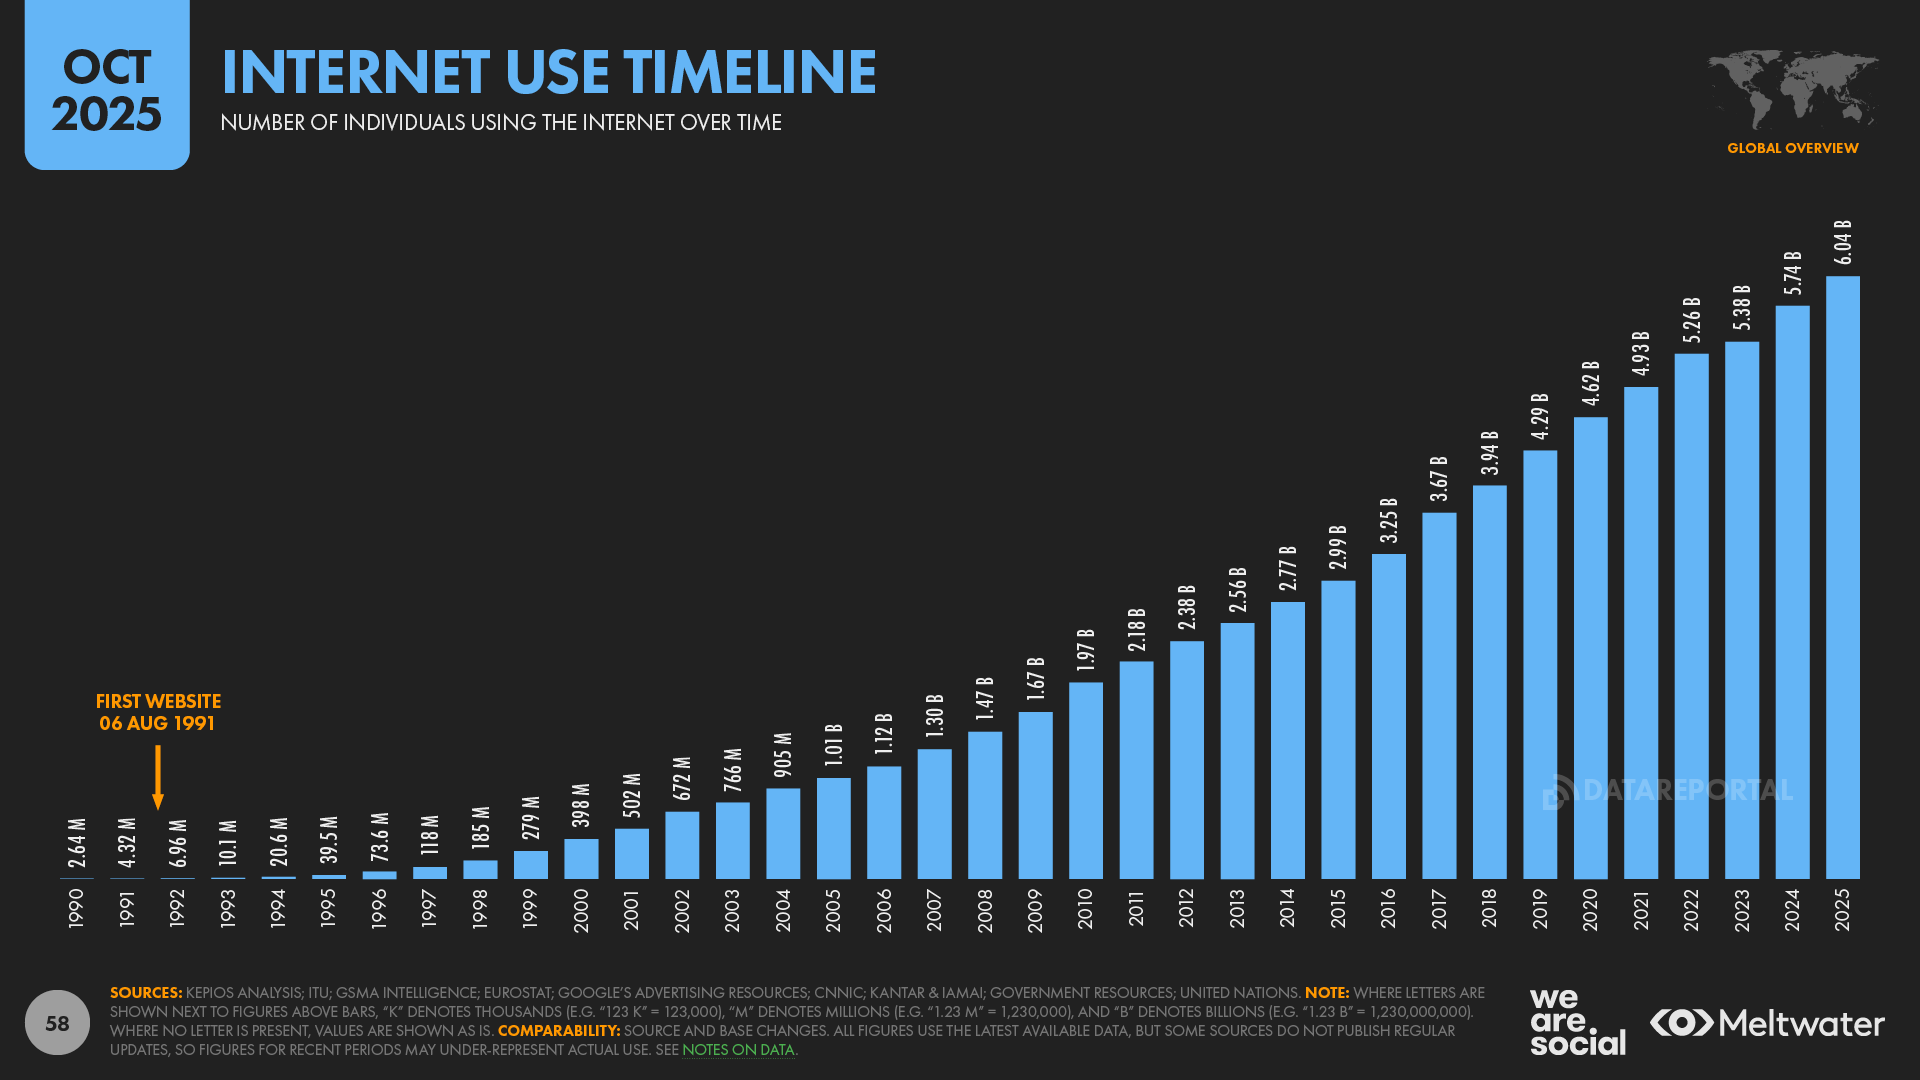
\includegraphics[width=0.6\textwidth]{internet_user_report_oct_25_datareportal.png}
    \caption{Number of internet users over the time}
    \label{fig:internet_user_report_oct_25_datareportal}
\end{figure}
However, as individual fiber capacity nears its theoretical Shannon limits, spectral multiplexing alone is often insufficient to satisfy massive localized traffic requirements. Consequently, network operators increasingly deploy "multifiber" or parallel-link configurations—utilizing multiple physical fiber pairs between adjacent nodes—to achieve a multiplicative increase in total throughput. While protocols like Link Aggregation (LAG) are traditionally utilized at higher network layers to duplex or group these connections for redundancy and increased bandwidth, managing these resources at the optical layer introduces significant complexity.

To handle the management burden of these high-capacity, multifiber infrastructures, the optical control plane has transitioned from static, manual configurations to highly automated, centralized management systems empowered by Software-Defined Networking (SDN). As DWDM technologies have matured, the traditional fixed-grid spectrum allocation—which assigns rigid, uniform channel spacing—has become a structural bottleneck. To overcome this, flexible-grid (flex-grid) architectures have emerged as the industry standard. By adhering to ITU-T G.694.1 standards, which utilize a precise 6.25 GHz slot granularity with 12.5 GHz slot width, flex-grid networks allow for elastic, demand-driven bandwidth allocation that vastly improves overall spectral efficiency \cite{itu694}.
\begin{figure}[htbp]
    \centering
    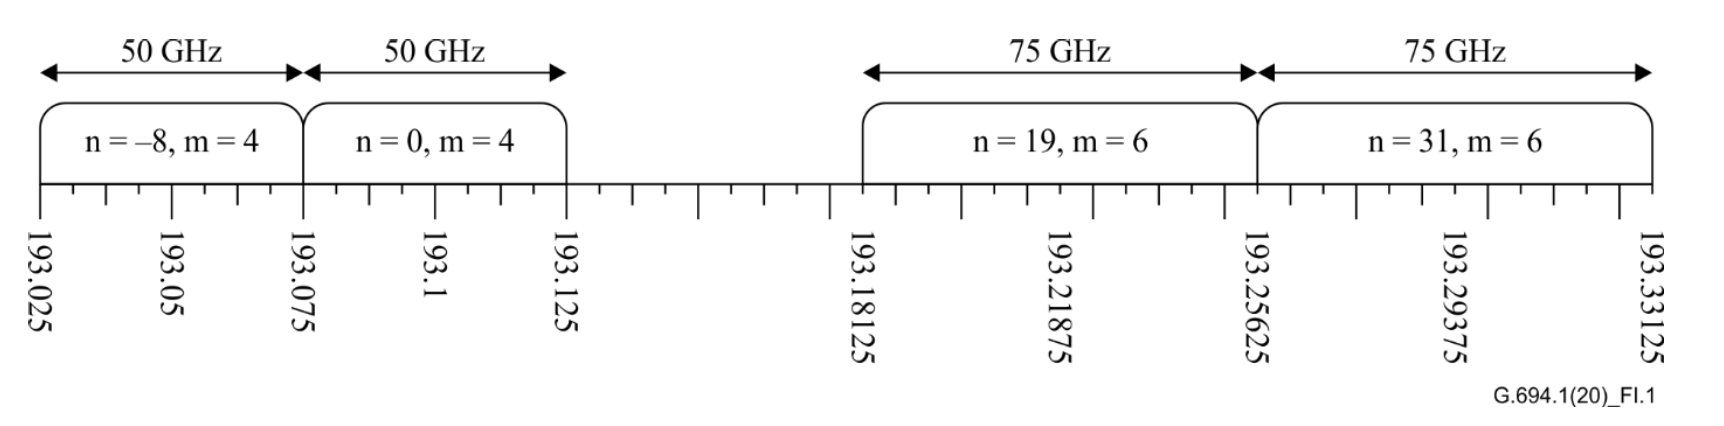
\includegraphics[width=0.7\textwidth]{example_of_flex_grid.png}
    \caption{An example of use of flexible the grid}
    \label{fig:example_usage_of_flex_grid}
\end{figure}
The deployment of flex-grid systems in long-haul backbone communications introduces substantial algorithmic complexity. In multi-hop networks, an optical signal must maintain both spectrum continuity—utilizing the same frequency across all links—and spectrum contiguity—utilizing adjacent frequency slots—from source to destination. This Routing and Spectrum Allocation (RSA) challenge is critically exacerbated in topologies featuring multiple parallel optical links between network elements, such as adjacent Reconfigurable Optical Add-Drop Multiplexers (ROADMs). When parallel links are introduced to a multi-hop architecture, the number of viable routing permutations increases exponentially. Consequently, traditional SDN controllers struggle to efficiently evaluate the availability of every 6.25 GHz slot across all possible path combinations, leading to severe computational bottlenecks and delayed provisioning times.

To resolve this critical scalability issue, this thesis proposes a novel approach by introducing the Parallel Optical Controller, a stateful microservice integrated directly into the TeraFlowSDN ecosystem. By leveraging advanced graph modeling techniques and a highly optimized bitwise spectrum intersection algorithm, this proposed method efficiently isolates available spectrum blocks across complex parallel routes. Ultimately, this solution effectively neutralizes the parallel link bottleneck, ensuring rapid, reliable, and highly scalable lightpath provisioning for next-generation optical networks.
\section{Motivation}
While extensive research has been conducted on Routing and Spectrum Allocation (RSA) in Elastic Optical Networks (EONs)\cite{algorithmsRSATaxonomy}\cite{efficientDynamicRSAEon},particularly concerning complex multi-hop lightpath provisioning\cite{heuristicWSAMultihop}—there remains a notable gap in the literature regarding the efficient management of multiple parallel optical links between adjacent devices. In traditional centralized control planes, such as those managed by other SDNs, parallel links are typically treated as isolated, individual entities rather than aggregated resources\cite{novelRoutingWSA}. Consequently, when a lightpath request is processed, the RSA algorithm is forced to evaluate the spectrum continuity of each parallel link independently\cite{efficientDynamicRSAEon}. This legacy approach is highly inefficient, as it triggers redundant, computationally heavy, back-and-forth calculations that severely degrade the controller's performance and scalability in dense optical topologies.

The primary motivation of this thesis is to fundamentally resolve this parallel link computational bottleneck within the emerging TeraFlowSDN ecosystem \cite{aboutTFS}. By addressing relative algorithmic inefficiency, the research aims to design a system capable of evaluating multiple parallel paths concurrently, significantly reducing the computational overhead required to find available flex-grid spectrum.

Furthermore, theoretical RSA optimization cannot be solved as just a theoretical math problem or a simulation using static data; its efficacy is strictly dependent on the acquisition of precise, real-time telemetry from the underlying physical layer. While modern optical networks are rapidly transitioning toward vendor-agnostic architectures unified by standardized data models such as OpenConfig\cite{openconfigYang} and OpenROADM\cite{openroadmYang}, a significant barrier remains in the practical deployment of centralized algorithms: hardware heterogeneity. Although these industry standards define common data models using YANG, individual equipment vendors frequently implement them with subtle variations in configuration hierarchies and telemetry reporting. Consequently, extracting uniform network state information—such as operational frequency ranges and transport capabilities—via a singular filtering procedure is often unfeasible in multi-vendor environments. This research addresses this disparity by bridging the gap between abstract path computation and physical hardware limitations through the extensive enhancement of device drivers within the TeraFlowSDN ecosystem. By refining the default driver logic and implementing a tiered approach that utilizes both standardized procedures and specialized, device-based handlers, this thesis establishes a more robust framework for multi-vendor support. These enhancements ensure that the proposed RSA algorithm is fed by accurate, model-driven telemetric data, effectively reconciling high-level computational logic with the practical complexities of diverse optical hardware management.
\section{Research Objectives}
To systematically address the challenges of Routing and Spectrum Allocation (RSA) over parallel optical links, this thesis is guided by the following core research objectives:
\begin{itemize}
    \item \textbf{Analysis of Flexible-Grid Standards:} To investigate the operational principles of flexible-grid optical networks, specifically adhering to the ITU-T G.694.1 standards regarding spectrum slot width and 6.25 GHz granularity.
    \item \textbf{Evaluation of SDN Optical Intent Provisioning:} To study how optical intents and lightpath requests are currently handled by popular, industry-standard Software-Defined Networking (SDN) controllers, identifying their limitations in dense, multi-link topologies.
    \item \textbf{Examination of TeraFlowSDN Device Drivers:} To conduct a comprehensive study of the telemetry and configuration mechanisms within TeraFlowSDN, with a specific focus on analyzing the OpenConfig and OpenROADM device drivers.
    \item  \textbf{Assessment of the Existing Optical Controller:} To critically evaluate the official OpticalController microservice currently operating within the TeraFlowSDN ecosystem, identifying its architectural constraints when processing complex optical intents.
    \item \textbf{Review of RSA Algorithmic Approaches:} To explore and analyze contemporary algorithmic strategies used to solve the RSA problem in multi-hop optical networks, evaluating their computational efficiency and spectrum assignment mechanisms.
    \item \textbf{Formulation of an Optimal Solution:} To synthesize the findings from the aforementioned studies and propose an optimal, highly scalable RSA framework that efficiently resolves the computational bottlenecks associated with parallel optical links.
\end{itemize}
\section{Thesis Contributions}
Building upon the established research objectives, this thesis makes several tangible contributions to the field of optical Software-Defined Networking (SDN), specifically addressing the computational bottlenecks associated with routing over parallel links. The core contributions of this work are summarized as follows:

\begin{itemize}
    \item \textbf{Enhancement of Optical Device Drivers:} A significant extension of the existing TeraFlowSDN device drivers, specifically the OCDriver (for OpenConfig devices) and the OpenROADM driver. This contribution includes the implementation of custom filters to extract vendor-agnostic telemetry—such as minimum and maximum operating frequencies, transport types (e.g., OCH, OMS), and flexible-grid parameters—directly from XML configurations, seamlessly integrating this data into an extended Context database schema.
    \item \textbf{Design of an Optimized RSA Algorithm:} The formulation and implementation of a highly scalable Routing and Spectrum Allocation (RSA) algorithm tailored for topologies with multiple parallel links. This includes utilizing the networkX library to construct multi-directed graphs that accurately represent parallel edges, alongside the introduction of a novel bitmap-based bitwise intersection method designed to rapidly compute the availability of contiguous 6.25 GHz spectrum slots across multiple hops.
    \item \textbf{Development of the ParallelOpticalController Microservice:} The creation, deployment, and integration of a novel, stateful microservice—the ParallelOpticalController—within the TeraFlowSDN microservices architecture. This dedicated controller autonomously processes complex optical intents, executing the advanced RSA algorithm to efficiently discover primary shortest paths and alternative route combinations without overwhelming the control plane.
    \item \textbf{Advanced Network Visualization and WebUI Integration:} To comprehensively upgrade the TeraFlowSDN Web User Interface (WebUI) to reflect the complex physical and logical states of the optical network. This objective focuses on developing visual representations of device endpoint capabilities, real-time spectrum slot availability (based on ITU-T 6.25 GHz granularity), multi-hop topological links, and the dynamic output of the RSA computation.
\end{itemize}
By fulfilling these objectives, this research aims to deliver an end-to-end solution that spans from low-level physical device configuration up to high-level algorithmic path computation and graphical user interaction.
\section{Organization of the Thesis}
The remainder of this thesis is logically structured to guide the reader through the theoretical background, the proposed algorithmic solutions, the system implementation, and the final evaluation. The document is organized as follows:
\begin{itemize}
    \item \textbf{Chapter 2:} Background and Literature Review provides the foundational concepts necessary to understand the research. It discusses the principles of Software-Defined Networking (SDN) in optical networks, introduces the TeraFlowSDN architecture, and details Optical Transport Networks (OTN) including WDM technology and ITU standards. The chapter concludes with a review of existing Routing and Spectrum Allocation (RSA) algorithms, highlighting the specific problems and limitations associated with parallel links.
    \item \textbf{Chapter 3:} Problem Definition and Proposed Algorithm formally establishes the research problem and introduces the mathematical formulation of the challenge. It details the graph modeling techniques used to represent topologies with parallel links and breaks down the proposed RSA algorithm, covering bandwidth computation, path discovery, bitmap-based spectrum allocation, and slot acquisition, followed by a thorough complexity analysis.
    \item \textbf{Chapter 4:} System Design and Implementation delves into the practical engineering and software architecture of the proposed solution. It outlines the modifications made to TeraFlowSDN—including device service enhancements for OpenConfig and OpenROADM, database schema extensions, and the RSA Computation Module. Furthermore, it details the development of the new Parallel Optical Controller microservice and the corresponding WebUI enhancements for spectrum visualization.
    \item \textbf{Chapter 5:} Testbed Setup and Deployment outlines the experimental environment used to validate the proposed system. It describes the physical and virtual infrastructure, the configuration of emulated transponders and ROADM devices, the setup of network topologies, and the deployment procedure utilizing MicroK8s.
    \item \textbf{Chapter 6:} Results and Evaluation presents a comprehensive analysis of the system's performance. It covers functional validation, computational performance, and spectrum utilization efficiency. The chapter also provides a throughput analysis, a comparative study against baseline approaches, and a statistical discussion of the results.
    \item \textbf{Chapter 7:} Conclusion and Future Work summarizes the primary contributions of the thesis, discusses the current limitations of the implemented system, and suggests potential directions for future research and development.
\end{itemize}
\chapter{Background and Literature Review}
This chapter establishes the theoretical foundation and contextual background for the research presented in this thesis, tracing the technological progression from foundational Optical Transport Networks (OTN) to modern automated control architectures. The review begins by examining the evolution of Wavelength Division Multiplexing (WDM), detailing the industry-wide transition from rigid, fixed-grid spectrum allocation to the highly efficient, elastic paradigms of flexible-grid (flex-grid) EONs. It contrasts traditional, decentralized optical control planes with the emergence of Software-Defined Networking (SDN), which provides the centralized intelligence required for dynamic resource management. Within this context, the chapter details the architectural components of contemporary SDN controllers, specifically focusing on the TeraFlowSDN ecosystem. A critical analysis of current Routing and Spectrum Allocation (RSA) methodologies follows, identifying a persistent research gap: the inability of traditional path computation and spectrum assignment logic to scale effectively when encountering multi-hop topologies with parallel optical links. Finally, the chapter introduces the \texttt{ParallelOpticalController} as a transformative solution within TeraFlowSDN, designed to resolve these computational bottlenecks and provide high-speed, constraint-aware provisioning for complex multifiber infrastructures
\section{Software Defined Network}
\subsection{SDN Architecture and Principles}
Software-Defined Networking (SDN) represents a fundamental paradigm shift in telecommunications, decoupling the network's control logic—the control plane—from the underlying packet or optical forwarding hardware, known as the data plane. This structural separation centralizes network intelligence into a software-based controller that maintains a global, real-time view of the network topology and its available resources. By abstracting the physical infrastructure through open, standardized Southbound Interfaces (SBIs) such as NETCONF or gNMI, SDN enables deep network programmability and dynamic orchestration of forwarding behaviors. This centralized management framework allows high-level applications to request network resources through Northbound Interfaces (NBIs) without requiring granular knowledge of the physical layer's complexity. Consequently, SDN provides the necessary architecture to achieve multi-vendor interoperability and agile service provisioning, transforming rigid physical infrastructure into flexible, automated, and software-governed assets.
\subsection{SDN in Optical Networks}
While initially designed for packet-switched networks, SDN principles have been aggressively adapted for the optical domain to create Software-Defined Optical Networks (SDON). Unlike packet networks, optical networks must manage analog physical layer impairments, wavelength continuity, and complex spectrum allocation constraints. SDON abstracts these physical layer complexities by decoupling the intelligent control logic—termed Optics Defining Software (ODS)—from the programmable physical hardware, known as Software Defined Optics (SDO) \cite{softwareDefinedOpticalNetwork}. This abstraction allows the central controller to dynamically provision lightpaths, tune variable transponders for specific modulation formats, and automatically configure advanced Reconfigurable Optical Add-Drop Multiplexers (ROADMs), successfully moving away from historically static, manually operated optical grids. To manage this complexity at scale, modern SDON deployments frequently adopt a Transport-SDN (T-SDN) architecture, this is often achieved through a hierarchical control structure \cite{largeScaleOpticalSDN}. In this model, lower-level controllers manage specific optical nodes, while a higher-level controller (such as ONOS) facilitates multi-vendor integration using standardized interfaces like the Transport API (T-API) over NETCONF and RESTCONF protocols.
Furthermore, breaking vendor lock-in is a critical focus of modern optical control planes and initiatives like the Open Disaggregated Transport Network (ODTN) utilize standardized YANG data models (such as OpenConfig and OpenROADM) to abstract heterogeneous hardware \cite{odtn}. This standardization enables the seamless, end-to-end integration of packet and optical layers across disaggregated white-box devices. Finally, as emphasized in "Network Slicing in SDN Networks," this centralized, programmable control is what ultimately enables advanced network virtualization. By leveraging SDON capabilities, operators can deploy multiple isolated logical slices over a single shared physical infrastructure, dynamically shaping traffic to guarantee specific Quality of Service (QoS) and performance isolation for varying applications.
\section{TeraflowSDN}
\subsection{Architecture and Ecosystem}
TeraFlowSDN (TFS) is a state-of-the-art, open-source SDN controller developed under the European Telecommunications Standards Institute (ETSI) to radically advance the orchestration of beyond 5G and 6G networks. Designed as a secure, cloud-native platform, TFS employs a microservices-based architecture orchestrated within Kubernetes environments, enabling individual control components to operate autonomously and scale independently. This inherent modularity provides an ideal ecosystem for integrating custom logic, such as vendor-agnostic device drivers and novel path computation engines. Furthermore, the architecture is explicitly engineered to seamlessly integrate with modern Network Function Virtualization (NFV) and Multi-access Edge Computing (MEC) frameworks, including ETSI OpenSourceMANO. By unifying network and cloud resource management, TeraFlowSDN equips telecom operators and hyperscale cloud providers with zero-touch automation, high business agility, and dynamic service provisioning across complex, multi-tenant optical and packet transport infrastructures.
\begin{figure}[htbp]
    \centering
    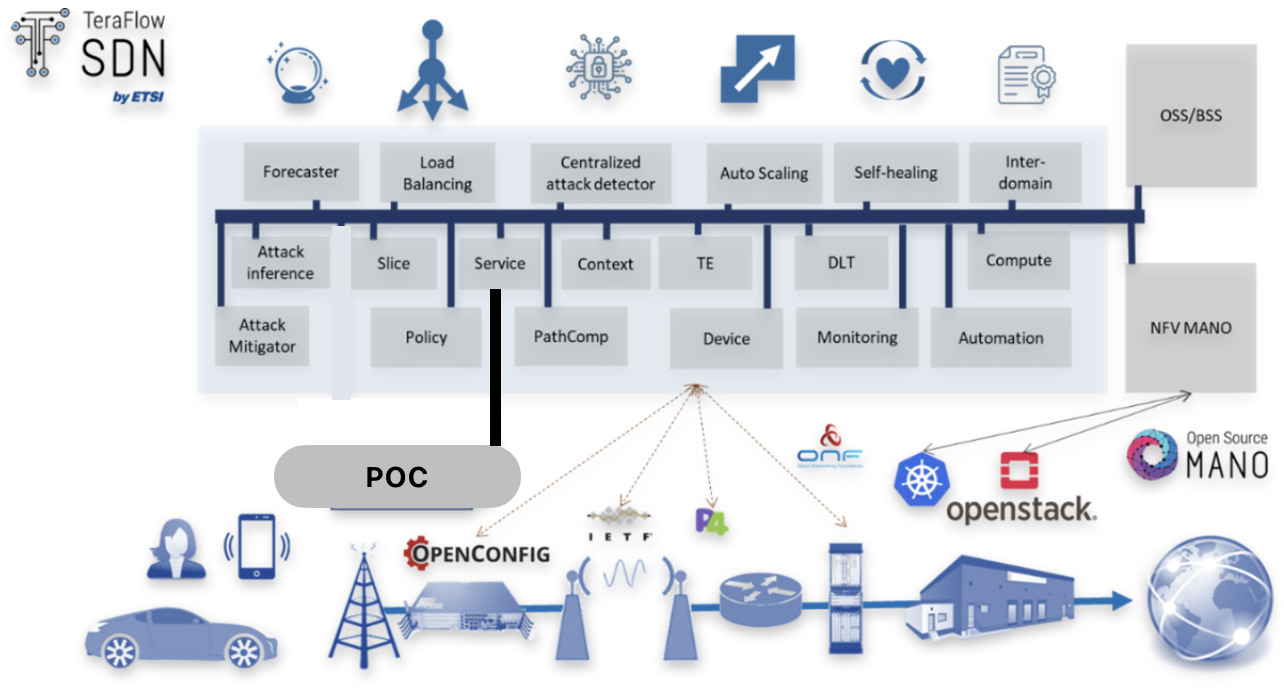
\includegraphics[width=0.6\textwidth]{tfs_architecture.png}
    \caption{TeraflowSDN Architecture}
    \label{fig:tfs_architecture}
\end{figure}
\subsection{Key services}
The TeraFlowSDN ecosystem relies on a highly coordinated suite of specialized microservices, communicating via Remote Procedure Calls (gRPC), to maintain network state and execute dynamic configurations. At the core of this architecture is the Context Service, which acts as the highly available, stateful storage mechanism maintaining the definitive global view of multi-domain topologies, devices, endpoints, and active network slices. Interacting closely with this centralized database is the Device Service, which manages all southbound interfaces by utilizing a modular framework of vendor-agnostic drivers—often leveraging NETCONF and OpenConfig models—to dynamically onboard and configure physical or emulated hardware. Furthermore, the Service Component oversees the end-to-end lifecycle of network connections by interpreting incoming connectivity requests and delegating cross-layer configurations to appropriate handlers. For optical transport infrastructures specifically, the OpticalController operates as a dedicated service to process complex optical intents, executing resource allocation algorithms such as Routing and Spectrum Assignment (RSA) to establish continuous and contiguous lightpaths across multi-hop networks. These fundamental operations are visually managed through a graphical WebUI that provides topology visualization and telemetry display, while the broader ecosystem is fortified by complementary microservices dedicated to machine learning-based security, distributed ledger technologies for multi-tenancy, and policy-driven automation to ensure robust, zero-touch network orchestration.
\section{Optical Transport Networks}
\subsection{WDM technology}
Wavelength Division Multiplexing (WDM), specifically Dense WDM (DWDM), is the foundational technology for modern high-capacity optical networks. DWDM enables the transmission of multiple data streams over a single optical fiber by modulating each stream onto a distinct wavelength (or color) of laser light. Historically, DWDM utilized a fixed-grid spacing, allocating rigid channel intervals of 50 GHz, 100 GHz, or even wider. However, as data rates increased and traffic patterns became more unpredictable, this rigid spacing resulted in inefficient spectrum utilization. To address this bottleneck, modern elastic optical networks (EONs) utilize flexible-grid (flex-grid) technologies\cite{opticalNetworksAndMangementControl}. As defined in the ITU-T G.694.1 standard, the flex-grid allows a mixed bit rate or mixed modulation format transmission system to allocate frequency slots with different widths, optimizing the spectrum for the specific bandwidth requirements of individual channels\cite{itu694}. This transition from fixed to flexible allocation is what necessitates advanced Routing and Spectrum Allocation (RSA) algorithms, such as the one proposed in this thesis, to dynamically manage the resulting variable-width spectrum blocks across complex, multi-fiber topologies.
\begin{figure}[htbp]
    \centering
    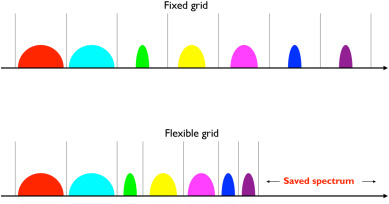
\includegraphics[width=0.6\textwidth]{dwdm_flex_grid.jpg}
    \caption{DWDM Flex-Grid Overview}
    \label{fig:dwdm_flex_grid}
\end{figure}
\subsection{ITU standards}
The implementation of these flex-grid networks is strictly governed by International Telecommunication Union (ITU) standards to ensure interoperability and consistent spectrum management. Specifically, the ITU-T G.694.1 Recommendation provides the definitive frequency grid for DWDM applications. Under this standard, the entire DWDM spectrum is anchored to a reference central frequency of 193.1 THz.
To enable elastic allocation, the standard defines a "frequency slot" as a contiguous frequency range characterized by its nominal central frequency and its total slot width. The architecture is built upon two critical granularities:
\begin{itemize}
    \item \textbf{Nominal Central Frequency Granularity:} The allowed central frequencies are defined by the formula $193.1 + n \times 0.00625$ THz, establishing a fine-grained granularity of 6.25 GHz to allow precise positioning of channels.
    \item \textbf{Slot Width Granularity:} The total width of any assigned frequency slot is defined by $12.5 \times m$ GHz, establishing 12.5 GHz as the minimum, indivisible building block for bandwidth allocation.
\end{itemize}
\subsection{Network elements (devices)}
The physical topology comprises two primary categories of optical nodes: terminal multiplexers (transponders and muxponders) and Reconfigurable Optical Add-Drop Multiplexers (ROADMs). In modern high-capacity optical networks, network endpoints are more precisely characterized as muxponders, which aggregate multiple lower-rate client-layer signals into high-speed optical channels suitable for DWDM transmission. These devices utilize bidirectional ports equipped with advanced pluggable transceivers that handle complex modulation and Forward Error Correction (FEC). While the telecommunications industry employs a diverse array of transceiver form factors and optical modules—such as QSFP, QSFP28, OpenZR+, and 400ZR—each offering varying frequency band support, capacity, and error correction capabilities, this thesis adopts a specific, standardized hardware profile for its emulation environment. Specifically, the emulated muxponder ports are modeled using the QSFP56-DD form factor equipped with Digital Coherent Optics, utilizing a 400GBASE-ZR Ethernet Physical Medium Dependent (PMD) sublayer and automated FEC. Although real-world deployments may feature heterogeneous transceiver capabilities, a foundational assumption of this research is that all muxponder ports are fully bidirectional and provide continuous, tunable frequency support across the entire C-band. This baseline ensures a uniform spectrum allocation space for evaluating the proposed RSA algorithms.
\begin{figure}[htbp]
    \centering
    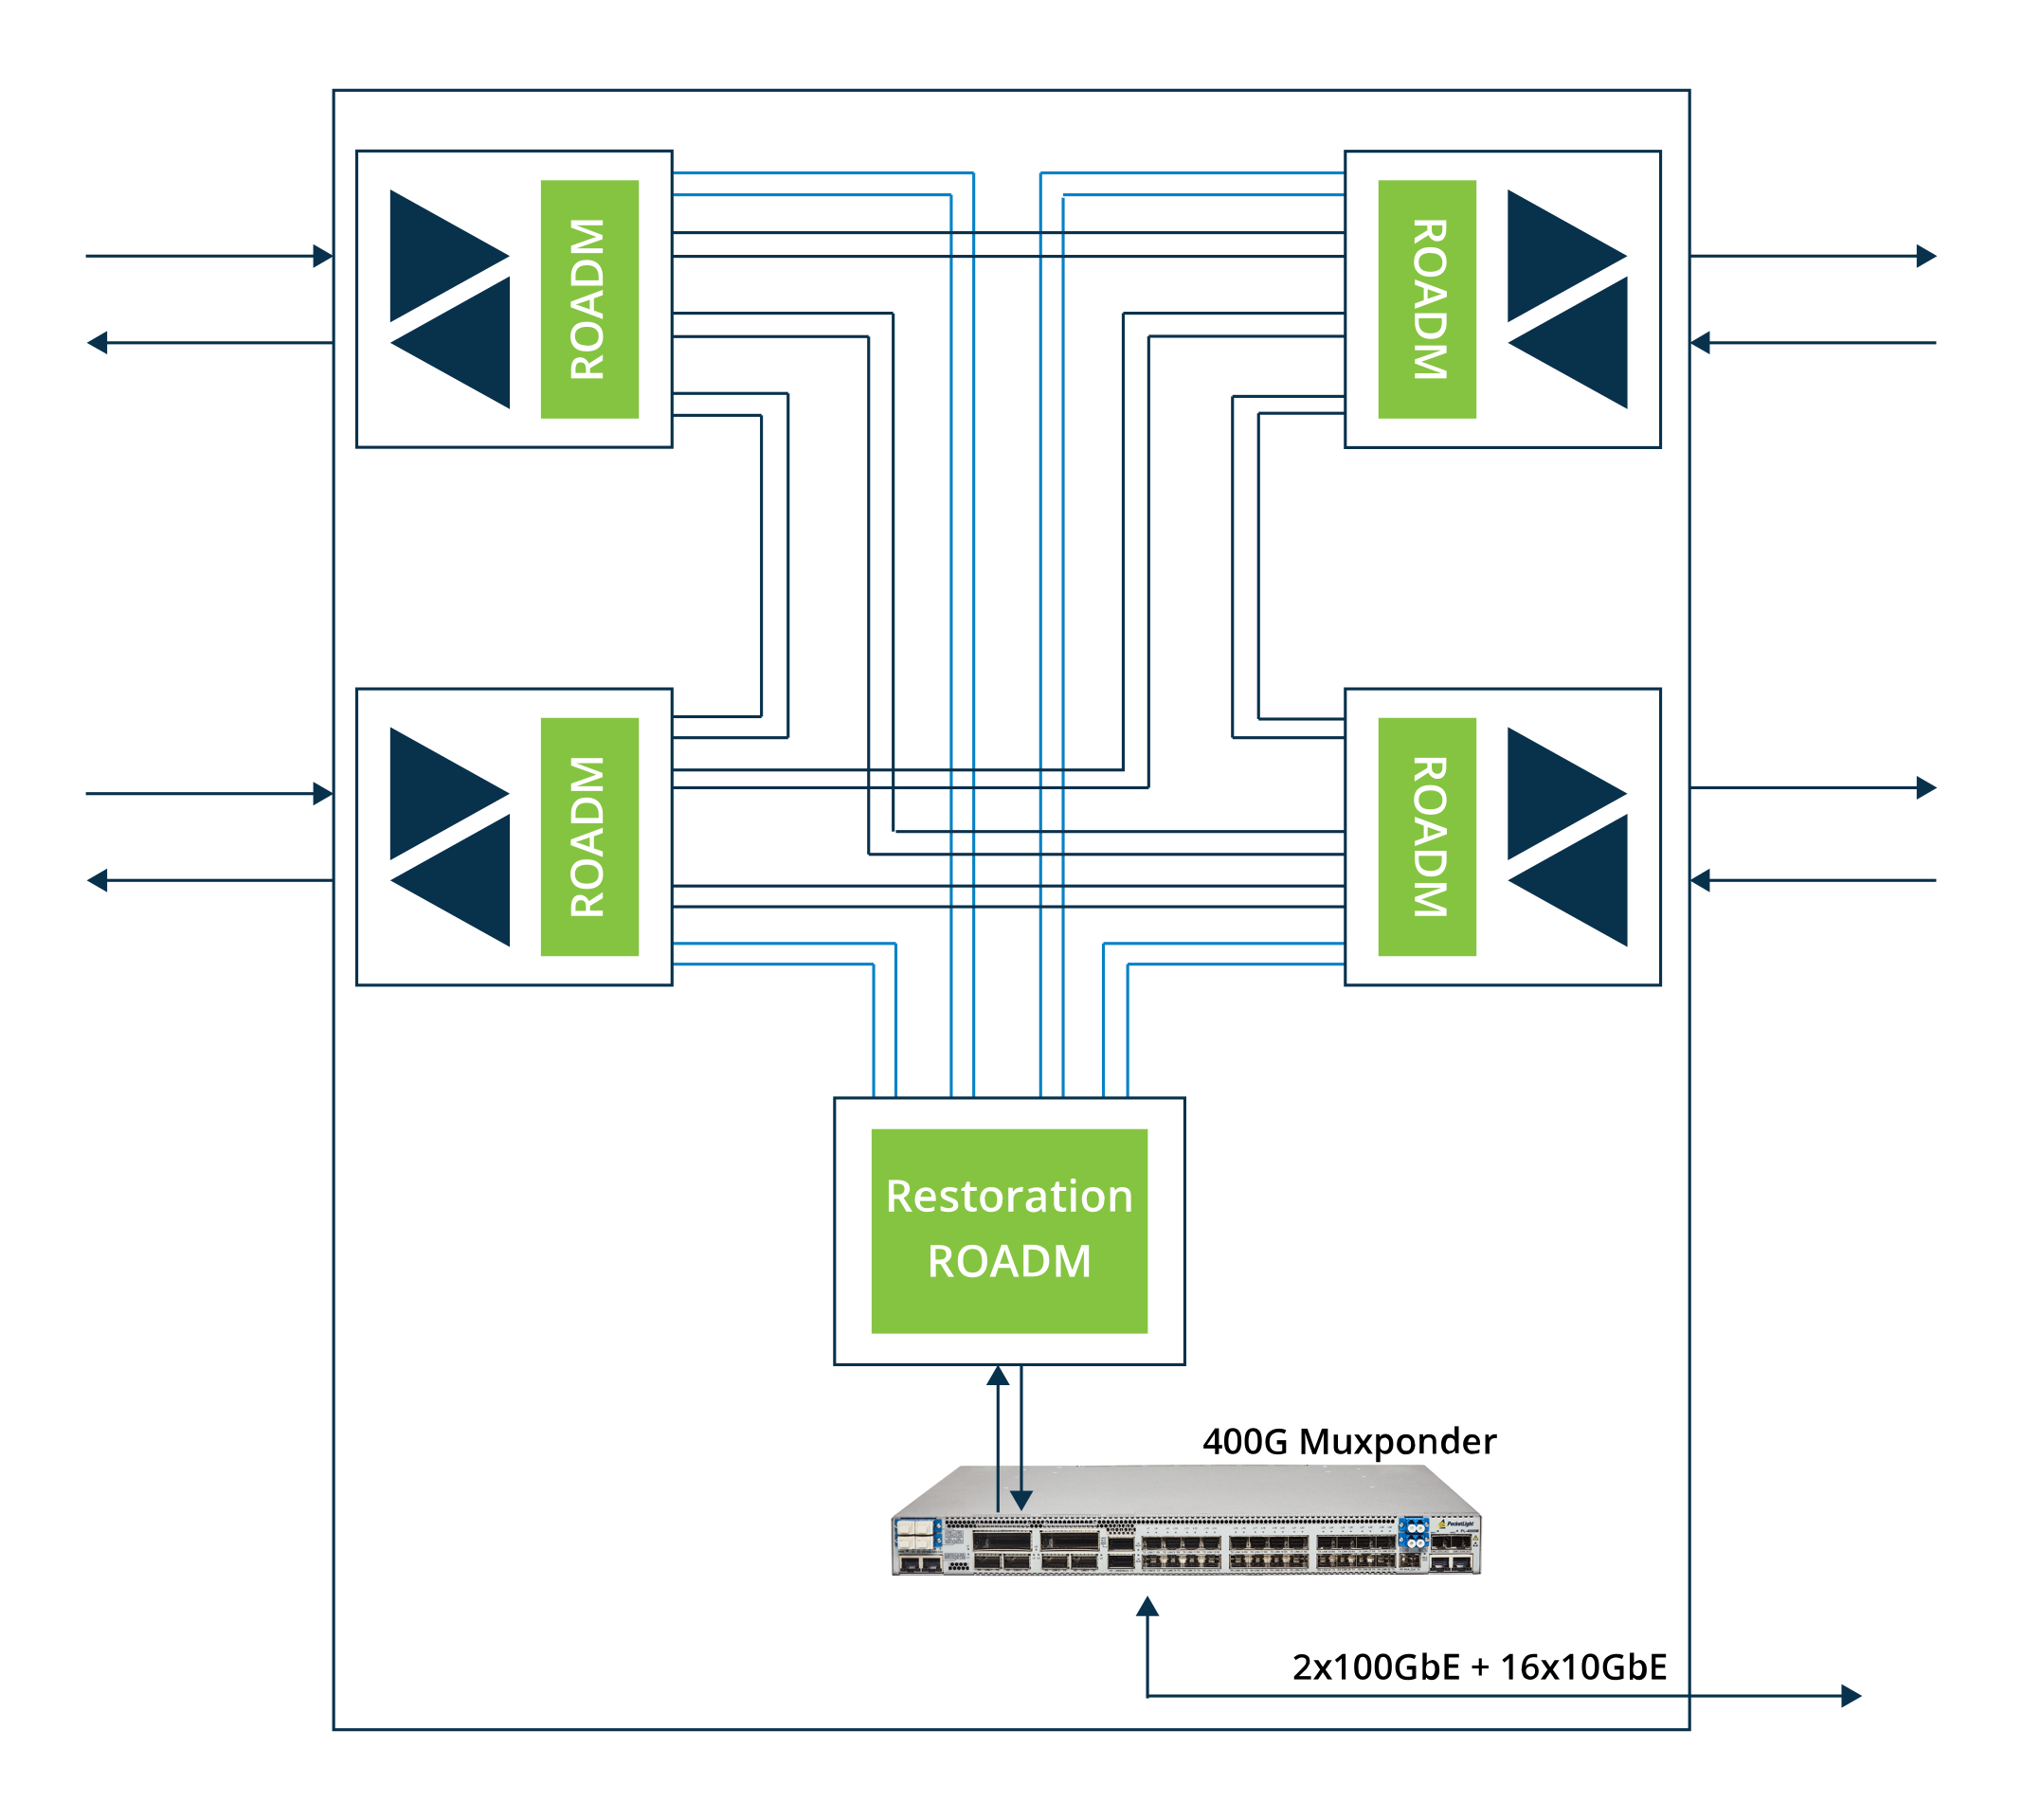
\includegraphics[width=0.6\textwidth]{roadm_muxponder.png}
    \caption{An example optical network}
    \label{fig:roadm_muxponder}
\end{figure}
Conversely, ROADMs serve as the optical switching backbone, enabling individual wavelengths to be dynamically added, dropped, or passed through a node entirely in the optical domain, thereby bypassing costly optical-to-electrical-to-optical (O-E-O) conversions. To accurately evaluate the Routing and Spectrum Allocation (RSA) algorithm on parallel links, it is necessary to establish strict assumptions regarding the internal architecture of these ROADMs. A typical ROADM architecture consists of Shared Risk Groups (SRGs) for local add/drop functionality and Direction Degrees (DEGs) equipped with Wavelength Selective Switches (WSS) for line-side routing. In the context of this thesis, physical fiber connections are only classified as strict "parallel links" if the ports originating from the same muxponder terminate at the same SRG and are routed outward through the exact same DEG of the ROADM. Under this specific topological constraint, the parallel fibers share an identical physical routing vector, making spectrum contiguity and continuity algorithms highly complex, as the spatial routing does not inherently resolve spectrum overlap. If the ports were to route through different DEGs, the spatial separation provided by distinct WSS hardware would allow for simple frequency re-use, thereby negating the specific parallel-link RSA constraints addressed in this study. Furthermore, to accommodate high-capacity throughput and scalability, the ROADM devices in this simulated environment are assumed to be wideband-capable, operating seamlessly across the entire S, C, and L (SCL) optical bands.
\subsection{Data models (configuration)}
To achieve true interoperability and break the traditional hardware lock-in imposed by proprietary management interfaces, modern optical equipment relies on standardized YANG data models. OpenConfig\cite{openconfigYang} and OpenROADM\cite{openroadmYang} have emerged as the two prominent industry standards used to formalize the representation of optical device configurations and operational states. By structuring parameters in universally understood XML or JSON formats, these models hide the underlying hardware idiosyncrasies from the control plane, allowing an SDN controller to parse telemetry and push configurations uniformly regardless of the equipment manufacturer. To manage the complexity of optical networking, these data models utilize strictly defined XML namespaces to isolate specific operational domains. Within the emulation environment of this thesis, the terminal devices (muxponders) primarily utilize the OpenConfig standard. For instance, the physical hardware hierarchy—such as form factors and transceivers—is defined under the \href{http://openconfig.net/yang/platform}{plaform-namespace}. Concurrently, the operational optics are managed via the \href{http://openconfig.net/yang/terminal-device}{terminal-device namespace}, which dictates precise parameters such as operational frequencies (e.g., 191.6 THz), target output power, and the logical channel assignments mapping Ethernet client traffic to Optical Transport Network (OTN) line ports.

Conversely, the emulated optical switches utilize the OpenROADM data model, which is specifically tailored to describe complex photonic switching architectures. Using namespaces such as \href{http://org/openroadm/device}{device namespace} and \href{http://org/openroadm/interfaces}{interface namespace}, the model accurately maps the internal ROADM topology. It defines critical switching components including circuit packs (such as twin Wavelength Selective Switches), Direction Degrees (DEGs), Shared Risk Groups (SRGs), and specific optical interfaces like Optical Transport Section (OTS) and Optical Multiplex Section (OMS). By adhering to these standardized schemas, the SDN controller is decoupled from vendor-specific command-line interfaces. Consequently, network operators can seamlessly deploy heterogeneous, multi-vendor optical topologies. A single controller can dynamically orchestrate an end-to-end lightpath by pushing standard OpenConfig XML payloads to tune a Cisco transceiver, while simultaneously pushing OpenROADM payloads to configure cross-connects on an Ericsson ROADM, effectively unifying the entire physical layer.
\section{Routing and Spectrum Allocation}
\subsection{Spectrum continuity and contiguity constraints}
Establishing a lightpath in an Elastic Optical Network (EON) requires solving the complex Routing and Spectrum Allocation (RSA) problem. In traditional fixed-grid DWDM networks, resource allocation—known as Routing and Wavelength Assignment (RWA)—was primarily concerned with satisfying a simple wavelength continuity requirement \cite{rsaHeuristicSliced}. However, the evolution to flexible-grid EONs introduces highly restrictive dual constraints that transform resource allocation into an NP-hard computational challenge \cite{rsaHeuristicSliced}. Regardless of the specific allocation policy utilized, every valid assignment in an EON must fundamentally satisfy three primary physical constraints \cite{algorithmsRSATaxonomy}:

\begin{itemize}
    \item \textbf{Spectrum Continuity:} This constraint dictates that the exact same frequency spectrum (the specific index of the allocated spectrum slots) must be utilized and remain identical across every single link along the end-to-end routing path \cite{algorithmResearchRSAONR}. However, in multifiber infrastructures featuring parallel links, this constraint presents a crucial operational nuance \cite{efficientDynamicRSAEon}. While the frequency index must remain identical end-to-end, the optical signal is permitted to shift spatially between parallel physical fibers at each hop, provided there are no internal switching restrictions at the optical cross-connects \cite{efficientDynamicRSAEon}.
    \item \textbf{Spectrum Contiguity:} The frequency slots assigned to a single lightpath must be strictly adjacent to one another within the frequency domain to form a contiguous "Slot Block". In modern implementations, algorithms treat individual frequency slots as fixed at a minimum width (typically 12.5 GHz) and group them contiguously to precisely match the variable bandwidth demands of the traffic \cite{algorithmsRSATaxonomy}.
    \item \textbf{Spectrum Non-Overlapping:} To prevent signal interference and data corruption, this constraint ensures that any specific frequency slot on a given physical fiber is allocated to a maximum of one active lightpath at a time \cite{efficientDynamicRSAEon}.
\end{itemize}
The tight coupling of the continuity and contiguity constraints often leads to severe spectrum fragmentation. Because of the strict contiguity requirement, having enough total available spectrum on a path is insufficient if those slots are scattered and fragmented. To enforce these rules without blocking new requests, advanced RSA algorithms manage both constraints simultaneously by treating the network state as a unified "allocation matrix". This allows the controller to search for the first available block of contiguous slots that spans uniformly across all physical edges along the chosen multi-hop route \cite{rsaFlexGrid}.
\subsection{Existing RSA algorithms}
As established, the strict enforcement of spectrum continuity and contiguity transforms network resource allocation into a highly restrictive, NP-hard computational challenge\cite{rsaHeuristicSliced}. To prevent severe spectrum fragmentation and the unfair blocking of high-capacity requests, intense research has been dedicated to developing sophisticated Routing and Spectrum Allocation (RSA) algorithms\cite{distanceAdaptive}. Over time, these algorithms have evolved from basic wavelength assignment models into complex, multi-metric optimization strategies designed to maximize network throughput and accommodate diverse, dynamic traffic demands\cite{algorithmsRSATaxonomy}. Early approaches sought to decouple the routing and assignment phases to mitigate computational bottlenecks. Foundational algorithms employed greedy heuristics and K-shortest paths to maximize single-hop traffic while strictly enforcing standard wavelength continuity\cite{heuristicWSAMultihop}. As networks transitioned to flex-grid EONs, researchers introduced offline traffic sorting heuristics to groom traffic more efficiently. For instance, the Minimum Hops with Least Slots (MHLS) algorithm prioritizes connection requests by calculating a sorting parameter\cite{rsaHeuristicSliced}:
\[
    NP=Hops \times Slots
\]
By serving "smaller" requests first, the algorithm minimizes overall blocked traffic\cite{rsaHeuristicSliced}. More dynamic approaches have integrated custom cost functions to balance multiple network metrics simultaneously. For example, the \texttt{FRSO-RSA} algorithm evaluates candidate alternative routes by actively steering traffic away from congested or unreliable paths using the following cost function\cite{failureProbability}:
\[
    cost_c = \alpha \times PF_c + (1 - \alpha) OU_c
\]
where $PF_c$ represents the physical failure rate of the path, $OU_c$ denotes the spectrum occupancy rate, and $\alpha$ acts as an adjustable weight parameter\cite{failureProbability}.
To combat the specific issue of contiguity-induced fragmentation, recent literature has shifted toward "next-state-aware" algorithms. Metrics such as Maximum Spectrum Completeness (MSC) are used to evaluate how a current assignment will impact future capacity, actively selecting routes that preserve large, unbroken blocks of spectrum \cite{maximumSpectrumCompleteness}. Other strategies introduce highly dynamic link-weighting mechanisms that actively draw traffic toward links harboring the largest unfragmented spectrum slices rather than just looking at total available capacity \cite{spectrumStatusAware}. When fragmentation inevitably occurs during the network's lifecycle, complex defragmentation algorithms utilizing Integer Linear Programming (ILP) and Resource Dependency Digraphs (RDD) are deployed to mathematically recalculate and shift existing lightpaths without altering their physical routes\cite{optimizingSpectrumAllocationEON}. Furthermore, advanced meta-heuristics like Genetic Algorithms and probabilistic models like Markov Decision Processes (MDP) have been explored to navigate massive solution spaces and predict network states\cite{routingModulation,adaptiveRSAFlex}.
\section{Problems with Parallel Links in RSA}
\subsection{Problem statement}
While the Routing and Spectrum Allocation (RSA) problem in optical networks has been extensively studied for years, the comprehensive integration of multi-fiber or parallel links between adjacent nodes remains an underexplored area. Technologies such as link aggregation and bandwidth duplexing have become increasingly common, introducing multiple physical connections between devices to meet escalating capacity demands. Specifically, to aggregate a higher number of optical channels, multiple parallel connections are routinely established between a muxponder and a Reconfigurable Optical Add-Drop Multiplexer (ROADM). A critical physical constraint in this architecture is that the same spectrum cannot be reused across parallel links that terminate at the same degree of a ROADM device without causing severe interference. Traditional RSA algorithms primarily focus on path computation, spectrum continuity, and spectrum contiguity across single-fiber logical links. However, they frequently fail to account for the spatial complexity introduced by multi-fiber or parallel-link topologies. Current RSA algorithms already face significant scalability and efficiency drawbacks in complex, highly meshed topologies; introducing parallel links exacerbates these challenges dramatically. In a multi-graph network featuring a uniform or variable number of parallel links between adjacent devices, the total number of possible path combinations from a source to a destination increases exponentially. Because signals routed over the same ROADM degree cannot share frequencies, a network controller must exhaustively calculate and verify the availability of every frequency slot across every parallel edge. Computing paths in such multi-dimensional scenarios can easily overwhelm current algorithms, resulting in massive computational overhead, unacceptable latency, and ultimately, a failure in dynamic lightpath establishment. Consequently, there remains a critical research gap in developing routing strategies that can navigate the spatial complexity of parallel links without crippling network efficiency.
\section{Current approaches and limitation}
To address the NP-hard complexities of optical network management, theoretical research has developed sophisticated Routing and Spectrum Allocation (RSA) algorithms designed to mitigate severe spectrum fragmentation and maximize throughput. These strategies have evolved from foundational, decoupled wavelength assignment models and offline traffic sorting heuristics, into dynamic, multi-metric optimization approaches that actively steer traffic away from congested or unreliable paths. Recent literature also heavily emphasizes "next-state-aware" metrics, dynamic link-weighting, and complex defragmentation models. However, extensive taxonomic reviews reveal a prevailing structural limitation: the vast majority of these theoretical solutions are designed exclusively for one-dimensional, single-fiber-per-link topologies. When applied to multi-fiber scenarios, these models must treat parallel links either as physically invalid aggregated bandwidth or as entirely separate logical links, inevitably triggering a state-space explosion and unmanageable computational complexity.

In practical deployments, industry-standard SDN controllers like ONOS\cite{odtnONOS} and OpenDaylight (ODL)\cite{odlTPCE} attempt to manage these topologies using robust, graph-based routing engines, yet they fundamentally struggle with the same spatial constraints. In both controllers, optical connections are treated as strictly matched port-to-port links; thus, multiple parallel fibers between the same devices are mapped as entirely distinct and independent topological edges. When computing routes via standard K-Shortest Path algorithms, the topology engine outputs every permutation of these parallel links as a completely independent path sequence. Consequently, the subsequent spectrum allocation phase applies strict isolation, evaluating spectrum continuity and contiguity sequentially on a strict per-path basis. If an allocation attempt experiences wavelength contention on one parallel link, the controller discards the effort and must iteratively re-run the entire RSA verification from scratch on the next topological path permutation. In complex, highly meshed topologies featuring multiple parallel links, this exhaustive, sequential path-by-path iteration causes exponential computational overhead, often leading to unacceptable latency and dynamic provisioning timeouts. These systemic shortcomings in both theoretical models and practical SDN implementations highlight a critical research gap, presenting the opportunity to design a deterministic, spatially-aware parallel optical controller within the TeraFlowSDN ecosystem that evaluates parallel ports concurrently to bypass sequential iteration and enable highly scalable lightpath establishment.
\section{Related work}
While the Routing and Spectrum Allocation (RSA) problem has been extensively explored to address strict spectrum continuity and contiguity constraints, existing literature and practical deployments exhibit a critical blind spot regarding multi-fiber topologies. Advanced theoretical heuristics—such as next-state-aware metrics and dynamic link-weighting—are overwhelmingly optimized for one-dimensional logical links. When extended to parallel-link environments, both theoretical models and industry-standard SDN controllers typically resort to exhaustive, sequential path-by-path iterations or restrictive offline computations, leading to severe latency and state-space explosion. To bridge this gap, this thesis introduces the \texttt{ParallelOpticalController} within the TeraFlowSDN ecosystem. By concurrently evaluating all available parallel ports at each hop rather than processing them as isolated topological sequences, the proposed architecture natively leverages the spatial domain to resolve RSA constraints in real time, bypassing sequential bottlenecks and enabling highly scalable, low-latency lightpath establishment for next-generation multi-fiber networks.
\chapter{Problem Definition and Proposed Algorithm}
This chapter formalizes the Routing and Spectrum Allocation (RSA) challenge within multi-graph optical topologies and presents the core algorithmic solutions developed for this thesis. It details the methodologies used to model physical networks with parallel links, compute required bandwidth and slots, discover optimal and alternative paths, and dynamically allocate spectrum using a novel bitmap intersection approach.
\section{Formal Problem Statement}
To address the complexities of lightpath provisioning in modern elastic optical networks, the physical topology must first be formalized into a mathematical model. The optical network is represented as a directed multi-graph, denoted as $G=(N,L)$. In this model, $N$ represents the set of optical network nodes (e.g., transponders, muxponders, and ROADMs), and $L$ represents the set of bidirectional physical optical links interconnecting these nodes. A defining characteristic of the targeted architecture is the presence of parallel links—multiple distinct physical fibers connecting the same node pair $(u,v)\in N$. Therefore, the edge set $L$ is defined such that multiple edges can exist between any two vertices, formally expressed as a multi-graph where a link $l\in L$ is defined by the tuple $(u,v,k)$, with $k$ serving as a unique identifier for a specific parallel fiber between nodes $u$ and $v$. Each link $l$ supports a total spectrum capacity divided into a set of frequency slots, $W$, adhering to standard ITU-T flexible grid specifications.

The network is governed by a centralized control plane, orchestrated by the TeraFlowSDN ecosystem. Within this environment, it is assumed that several active lightpaths, denoted as $LP_i(N_s, N_d)$, already exist, utilizing specific continuous and contiguous blocks of spectrum $w_i\subset W$ across various links to connect source nodes $N_s$ to destination nodes $N_d$. The core challenge arises when a new lightpath request is submitted to the controller. The controller cannot simply compute the shortest path by treating the network as a standard simple graph. It must account for the current spectral state of the network, recognizing that certain links may be nearing capacity. Most critically, the routing algorithm must resolve the stringent physical constraints imposed by parallel links terminating at the same ROADM device. Specifically, in modern deployments, multiple parallel fibers originating from the same muxponder are frequently directed to the same Shared Risk Group (SRG) and subsequently multiplexed into the same Degree (DEG) of a ROADM. Because these signals share the same physical amplification and switching infrastructure within the DEG, they are subject to strict spectral isolation constraints. If active lightpaths currently utilize a specific set of frequency slots on link $l_(u,v,1)$, those identical frequencies cannot be reused on a parallel link $l_(u,v,2)$ connecting the same devices, as doing so would result in severe optical interference. Therefore, when establishing a new lightpath across a parallel edge $l_(u,v,k)$, the routing logic cannot evaluate the spectrum availability of link $k$ in isolation. It must perform a concurrent evaluation of the entire spatial bundle of parallel links connecting $u$ and $v$ to ensure that the newly allocated contiguous spectrum block does not overlap with any frequencies currently active on sibling links $i$ or $j$. The formal objective of the \texttt{ParallelOpticalController} is to efficiently compute the optimal routing path and allocate the necessary contiguous spectrum for incoming requests, specifically navigating the multi-dimensional constraints of parallel links, while minimizing overall network blocking probability and computational latency.
\section{Graph Modelling with Parallel Links (topologies)}
To efficiently navigate the multi-dimensional constraints established in the formal problem statement, the \texttt{ParallelOpticalController} avoids performing complex computations directly on the raw physical topology. Instead, the topological graph is logically segregated into specialized, abstracted versions. Acting as the centralized intelligence of the network, the TeraFlowSDN ecosystem provides the real-time database and telemetry required to construct, filter, and dynamically update these graphical models prior to processing any lightpath request. The core topology is first logically abstracted into an available-resource graph, denoted as $G_{free}$. The purpose of $G_{free}$ is to immediately prune physical resources that cannot mathematically support a new connection, thereby shrinking the search space. During its construction, the controller queries the TeraFlowSDN database and actively excludes fully occupied Optical Multiplex Section (OMS) links between ROADMs, as well as currently utilized Optical Channel (OCH) ports between muxponders and ROADMs. The resulting $G_{free}$ remains a multi-graph containing parallel links, but it strictly represents the network's actual residual capacity. While $G_{free}$ accurately reflects available resources, executing shortest-path algorithms directly on a dense multi-graph introduces significant, often exponential, computational overhead. To bypass this state-space explosion, $G_{free}$ is further abstracted into a simplified graph, denoted as $G_{simple}$. In this reduction, all parallel physical fibers connecting any adjacent node pair (u,v) are collapsed into a single representative logical edge. This transformation allows the controller to rapidly execute standard shortest-path and alternative-path computations (such as Dijkstra's shortest path algorithm) to discover the optimal topological routes from the source to the destination. Crucially, $G_{simple}$ is used strictly for topological path discovery, not for spectrum allocation. Once the candidate node-to-node routes are identified, the controller projects these paths back onto the multi-graph $G_{free}$ to perform the actual Routing and Spectrum Allocation (RSA). By evaluating the physical routes against $G_{free}$, the controller natively re-introduces the spatial domain—allowing it to concurrently evaluate all parallel fibers for a given hop. This dual-graph methodology ensures that the path finding phase remains computationally lightweight, while the final RSA phase mathematically guarantees that utilized spectrum is accurately nullified and the contiguity constraints are reliably satisfied across parallel links.
\section{Proposed RSA Algorithm}
The proposed Routing and Spectrum Allocation (RSA) algorithm operates through a sequence of integrated stages to dynamically provision lightpaths. The process is initiated when a service request is submitted via the TeraFlowSDN WebUI using a JSON descriptor. The controller parses this descriptor to extract critical constraints, such as the requested bandwidth and the hop-count limit for alternative path computation. Following this extraction, the algorithm systematically executes bandwidth and slot calculation, topological path discovery, and spatial spectrum allocation analysis across parallel links. Finally, rather than forcing an automated assignment, the architecture presents the computed valid path permutations intuitively via the control plane, allowing the network operator to explicitly select the desired spatial route for final spectrum acquisition and assignment.
\begin{figure}[htbp]
    \centering
    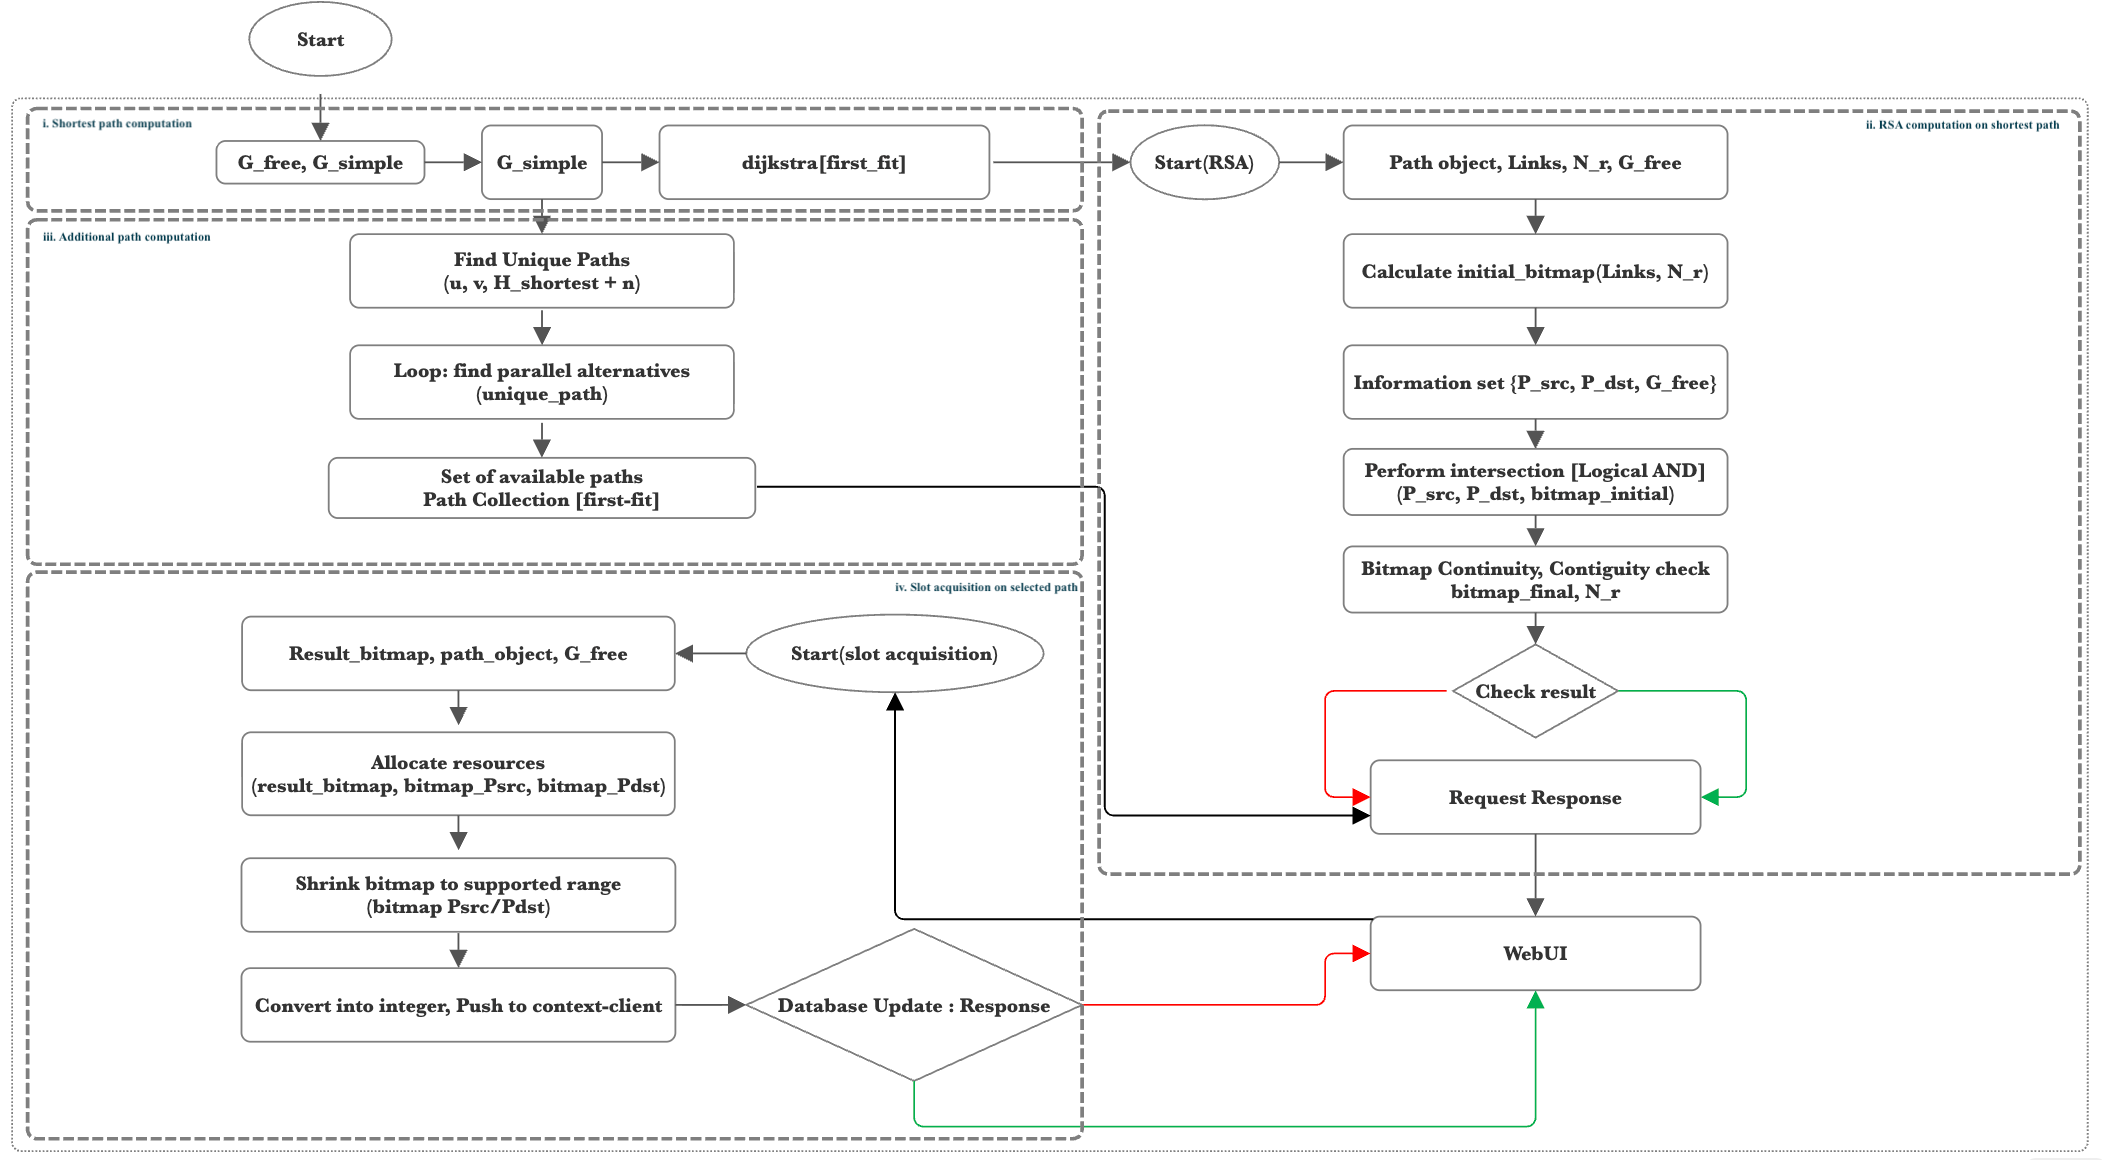
\includegraphics[width=1\textwidth]{full_algo_er.png}
    \caption{RSA operation using ParallelOpticalController in TeraFlowSDN}
    \label{fig:full_algo_er}
\end{figure}
\subsection{Bandwidth \& Slot Computation}
The initial phase of the proposed algorithm determines the required spectral bandwidth ($B_r$) for the requested optical service. Upon receiving a connection request, the controller extracts the target transmission bitrate ($R_b$), expressed in Gigabits per second (Gbps), directly from the submitted TeraFlowSDN service descriptor. The required bandwidth is then mathematically derived using the following formulation:
\[
    B_r = \frac{R_b}{n}(1 + \alpha)
\]
where $n=log_2(M)$, and M represents the specific modulation format utilized. While several factors influence the required bandwidth calculation \cite{ntiaBandwidth}, this standard formula simplifies the process for the controller.

Once the required bandwidth $B_r$ is established, the controller computes the discrete number of frequency slots ($N_r$) needed to accommodate the lightpath. In accordance with ITU-T flexible grid standards, while 12.5 GHz typically represents the minimum routable spectrum width, the nominal central frequency granularity of 6.25 GHz is utilized as the fundamental unit for this computation. This finer 6.25 GHz granularity is deliberately adopted to streamline the mathematical modeling and facilitate the subsequent bitmap-based spectrum assignment logic. The required number of slots is calculated as follows:
\[
    N_r = \frac{B_r}{6.25}
\]
Upon completion of this phase, the computed parameters, $B_r$ and $N_r$, are temporarily cached within the controller's operational memory. These values serve as the primary spectral constraints for the ensuing topological path discovery and spatial spectrum allocation phases.
\subsection{Path Discovery}
Following the determination of the required bandwidth and frequency slots, the controller advances to the topological path discovery phase. To perform fast and computationally efficient routing, the algorithm leverages NetworkX\cite{networkX}, a robust and highly optimized Python library designed for complex network analysis. During this phase, the routing engine queries the simplified graph abstraction, $G_{simple}$—where parallel physical fibers are collapsed into single logical edges. By routing over $G_{simple}$ rather than the raw physical multi-graph, the controller effectively prevents the state-space explosion and latency bottlenecks that plague traditional routing algorithms. The path computation engine is designed to execute two distinct routing operations to provide the user with maximum flexibility: it first identifies the absolute shortest path, and subsequently computes a set of viable alternative routes. This alternative path computation is governed by a user-defined hop-relaxation constraint, formulated as $H_{shortest}+n$, where $H_{shortest}$ represents the hop count of the primary shortest path and $n$ is a positive integer configured via the TeraFlowSDN service descriptor. The algorithm filters the topology to discover and validate alternative routes that strictly conform to this exact hop-count limit.

Once these node-level routes are successfully discovered in $G_{simple}$, the controller projects them back onto the available-resource multi-graph, $G_{free}$. Naturally, in a multi-fiber environment, a single node-to-node logical route expands into multiple physical path permutations between the source $(N_s)$ and destination $(N_d)$ devices. For standard operational deployment within the TeraFlowSDN ecosystem, the controller is configured to default to the first valid physical path object among these parallel permutations that satisfies the spectral constraints. However, to comprehensively evaluate the controller's spatial awareness, several alternate spatial selection strategies have been investigated, with their statistical impacts on network performance and blocking probability detailed in the subsequent analytical sections of this thesis.
\subsection{Bitmap-Based Spectrum Allocation}
Upon successful path discovery, the controller initiates the spectrum allocation phase using the primary shortest-path object derived from Dijkstra's algorithm, along with the previously computed slot requirement, $N_r$. While the controller defaults to evaluating the primary shortest path, RSA computation for any discovered alternative routes can be executed subsequently at the operator's discretion. The allocation process begins by querying the controller's internal cache to retrieve the real-time operational state of all physical links comprising the selected path object. The foundational step in this RSA methodology is establishing a uniform spectral reference framework. The controller analyzes the path to identify the maximum spectral band supported by any traversed device. Within the cache, the current spectrum utilization of each port is stored not just as discrete slots, but mathematically encoded as an integer value representing a binary sequence. This integer, referred to as the \texttt{bitmap-value}, is calculated using the following formulation:
\[
    \text{bitmap-value} = 2^N - 1
\]
The integer representing the widest supported operational band (typically the C+L band) is designated as the \texttt{bitmap\_initial}. This value establishes the maximum bit-length reference for all subsequent logical operations. A defining feature of this RSA algorithm is its native, unconditional sensitivity to multi-fiber topologies. Regardless of whether a specific hop explicitly utilizes multiple fibers, the algorithm inherently executes a parallelism check, ensuring that spectrum continuity and contiguity are dynamically evaluated across all available spatial dimensions between adjacent nodes. For a given hop along the path from source $N_s$ to destination $N_d$, the controller aggregates all available source ports into a set $P_{src}$ and all corresponding destination ports into a set $P_{dst}$. The current spectrum utilization of each port is retrieved as its integer \texttt{Bitmap\_value} and converted into its binary representation. To ensure mathematical alignment, each binary sequence is zero-padded or expanded to perfectly match the bit-length of the reference \texttt{bitmap\_initial}. Once aligned, the controller executes a concurrent bitwise intersection (logical AND operations) across the expanded bitmaps of all eligible source and destination ports within that hop. This concurrent spatial evaluation collapses the multi-fiber complexity into a single, unified mathematical representation, yielding a definitive \texttt{bitmap\_final}. This \texttt{bitmap\_final} sequence explicitly maps the continuous and contiguous spectrum gaps that are simultaneously available across the entire parallel link bundle. The controller then applies a standard First-Fit policy to the \texttt{bitmap\_final} sequence to identify the lowest-indexed contiguous block of zeros (available spectrum) that meets the required length $N_r$. The results of this deterministic spatial-spectral evaluation, including the final computed bitmap and the corresponding physical path hops, are subsequently relayed to the TeraFlowSDN WebUI for operator review.
\subsection{Slot Acquisition \& Assignment}
The final phase of the proposed RSA algorithm transitions from computation to operational execution, facilitating the actual acquisition and assignment of spectral slots. Rather than autonomously enforcing an allocation, the architecture employs an interactive, operator-in-the-loop paradigm. The network operator is presented with the computed primary and alternative path objects—along with their corresponding available spectrum blocks—and is granted the flexibility to explore these options and explicitly select the preferred spatial route via the TeraFlowSDN WebUI. Upon operator's confirmation, the controller initiates the slot acquisition protocol for the selected path. It retrieves the current link information for the chosen route and updates the spectral state by converting the newly allocated continuous blocks from their binary bitmap representations back into integer values. These updated integer values are subsequently pushed to the centralized database via the TeraFlowSDN Context component (e.g., using the Context client API) to accurately reflect the network's newly diminished capacity.

Concurrently, the controller executes a series of state updates across the topology. At the central database level, the specific spatial device ports utilized by the lightpath are flagged as \texttt{used=True} to prevent future routing collisions. At the orchestration level, the computed lightpath object is transitioned to an "active" state, and the overarching service request is formally marked as "ACTIVE" within the central knowledge base. Operators can subsequently monitor these allocated resources, port usages, and path details through the WebUI. Crucially, within the current scope of this implementation, the \texttt{ParallelOpticalController} operates strictly as a control-plane and orchestration entity. While it comprehensively updates the centralized database and topological state to enforce resource locking, it does not currently generate or transmit southbound physical configuration commands (such as NETCONF or RESTCONF) to alter the hardware interfaces of the physical optical devices. All spectral acquisition and state management are logically enforced at the controller level.
\section{Complexity Analysis}
The computational efficiency of the proposed \texttt{ParallelOpticalController} is fundamentally anchored in its ability to decouple topological routing from spatial spectrum allocation. The initialization phase, which constructs the abstracted multi-graph $(G_{free})$ and simplified routing graph $(G_{simple})$, traverses the network state in strictly linear time, $O(|N|+|L|)$—effectively $O(n)$ relative to the total topology size ($n$ represents a unit consisted of $N,L$)—ensuring predictable memory and processing scaling as physical devices and links are added. Subsequently, by executing topological path discovery exclusively on the collapsed graph $G_{simple}$, the controller avoids the state-space explosion typical of multi-graph environments, maintaining Dijkstra's standard log-linear time complexity of $O(|L_{simple}|+|L \times logL|)$ (where $L_{simple}$ represents the links involved in the shortest-path). The most significant computational breakthrough, however, emerges during the Routing and Spectrum Allocation (RSA) phase.

While traditional SDN implementations evaluate multi-fiber topologies sequentially—resulting in an exponential time complexity of $O(L_{parallel}^H)$, where $L_{parallel}$ represents the number of parallel links per hop and $H$ denotes the path length(measured in hops)—the proposed algorithm evaluates spatial bundles concurrently. Because the bitwise intersection mathematical logic resolves spectral contiguity across all parallel ports in constant O(1) time at the CPU hardware level, the overall time complexity of the RSA phase is strictly bounded by $O(L_{parallel}\times H)$. This additive, linear scaling with respect to path length and fiber density, coupled with a minimal spatial footprint of $O(N+L)$ for graph storage and negligible auxiliary memory for the binary string operations, mathematically guarantees that the controller can provision complex, multi-fiber lightpaths without succumbing to the exponential latency bottlenecks inherent in conventional routing algorithms. To empirically validate these theoretical claims, comprehensive performance tests were conducted across varying network topologies, including well-known reference networks such as the Pan-European (PANEU) and NSFNet models. As demonstrated in the results below, the controller successfully maintains the mathematically established time and space complexities, exhibiting highly efficient scaling even when multi-fiber parallel links are introduced. Ultimately, the convergence of theoretical analysis and empirical performance metrics confirms the robust computational efficiency of the \texttt{ParallelOpticalController}. By leveraging concurrent spatial evaluation to eliminate sequential processing bottlenecks, the architecture ensures highly scalable, real-time lightpath provisioning capable of meeting the rigorous demands of next-generation, multi-fiber elastic optical networks.
\chapter{System Design and Implementation}
This chapter bridges the theoretical algorithms established previously with their practical application, providing a comprehensive technical overview of the software architecture engineered to natively support multi-fiber parallel links. It systematically details the structural enhancements integrated into the TeraFlowSDN ecosystem, the development of the underlying Routing and Spectrum Allocation (RSA) computational modules, and the operational deployment of the novel \texttt{ParallelOpticalController} microservice.
\section{Modifications to TeraFlowSDN}
To accommodate the complex spatial and spectral constraints of multi-fiber topologies, several core components of the TeraFlowSDN control plane required structural modifications. These enhancements ensure that the central database maintains a highly accurate, normalized representation of the physical optical layer.
\subsection{Enhancement of the DeviceService}
To accommodate the complex spatial and spectral constraints of multi-fiber topologies, several core components of the TeraFlowSDN control plane required structural modifications. These enhancements ensure that the central database maintains a highly accurate, normalized representation of the physical optical layer.
Modern elastic optical networks are inherently heterogeneous, relying on equipment from various manufacturers. While the industry utilizes standard YANG data models for device configuration and telemetry, the expansive scope of YANG allows different vendors to adopt significantly different internal data structures and naming conventions. Consequently, relying on a monolithic data extraction technique to parse equipment capabilities is unreliable and often fails to capture the granular optical parameters required for advanced RSA computation. To overcome this interoperability challenge, this thesis introduces a novel, dynamically adaptable data extraction technique integrated directly into the \texttt{DeviceService} component of TeraFlowSDN, which is responsible for orchestrating device drivers. Rather than applying a uniform parsing rule, the augmented \texttt{DeviceService} identifies the specific vendor and hardware model of the connected equipment and applies a tailored extraction profile. To maintain system robustness and ensure backward compatibility with uncharacterized or generic optical equipment, a default extraction methodology is enforced whenever a specific vendor signature is not recognized.

Following the initial data extraction, the driver logic applies a rigorous normalization phase. A standardized naming convention is forcefully applied to all identified transport channels, neutralizing any vendor-specific nomenclature discrepancies before the data enters the centralized TeraFlowSDN context database. Furthermore, the driver-level extraction mechanisms were heavily revised to explicitly capture the exact parameters required by the proposed \texttt{ParallelOpticalController}. Critical operational data—including the specific channel type, total spectral capacity, real-time slot availability, and precise physical channel-to-endpoint (port) mappings—are now mapped directly into the device's operational state. By systematically resolving and normalizing these attributes at the lowest level of the control plane (the driver level), the overarching controller is guaranteed a clean, unified, and highly accurate topological state, which is crucial for the efficient execution of the bitmap-based RSA algorithm.
\subsection{Context Service \& Database Schema Extensions}
Within the TeraFlowSDN architecture, the \texttt{ContextService} functions as the centralized repository and primary communication hub, orchestrating all persistent database transactions and cross-service data propagation. Because the device drivers were enhanced to capture highly granular, vendor-specific optical parameters, the underlying database schemas required corresponding structural extensions to accommodate and permanently store this influx of new telemetry. Consequently, the core data models within the \texttt{ContextService} were significantly augmented with novel attributes tailored explicitly to support the proposed spatial Routing and Spectrum Allocation (RSA) algorithm. Critical operational parameters—such as explicit physical endpoint indices, discrete flexible-grid frequency details, integer-encoded spectrum utilization bitmaps, and expanded hardware capability metrics—are now persistently recorded within the context database immediately following their extraction at the driver level. These newly modeled attributes form the foundational dataset required for the controller's multi-dimensional path and spectrum computations. To ensure this augmented dataset is securely and rapidly accessible across the distributed SDN control plane, the overarching Protocol Buffer (protobuf) definitions were substantially revised. By updating and recompiling these protobuf schemas, the system guarantees seamless, high-speed gRPC communication between internal components. This critical integration allows the \texttt{ParallelOpticalController} to instantly and reliably retrieve the complex spectral and spatial state of the multi-fiber network, thereby enabling real-time, mathematically accurate lightpath provisioning.
\section{Algorithmic Core and Helper Modules}
While the \texttt{ParallelOpticalController} operates as a high-level orchestration micro-service within the TeraFlowSDN ecosystem, its underlying computational intelligence—often conceptualized as the "brain" of the controller—is systematically distributed across a suite of specialized Python submodules. Rather than functioning as a monolithic script, the controller relies on these distinct internal layers working in tandem to execute complex spatial and spectral logic.

To maintain modularity and reusability, these helper functions are categorized into two domains: universally shared libraries and controller-specific core modules.
\subsection*{\small Shared Utility Modules}
To ensure strict compliance with physical layer protocols across the entire control plane, the system introduces \texttt{ITUStandards.py}. This module encapsulates the comprehensive ITU-T specifications for DWDM flexible-grid communications. During the device discovery and driver extraction phase (as detailed in Section 4.1.1), this module provides the definitive reference parameters necessary to accurately map physical hardware endpoints into standardized database formats. Complementing the standards definitions is \texttt{RSATools.py}, which provides a robust library of utility functions designed to parse and align this standardized physical data against the specific parameters of incoming lightpath requests (e.g., converting requested bitrate into required frequency slots). Because these foundational mapping and conversion operations are critical across multiple stages of the network lifecycle, both \texttt{ITUStandards.py} and \texttt{RSATools.py} are deployed as shared dependencies utilized by the \texttt{DeviceService}, the \texttt{WebService} (for accurate WebUI representation), and the \texttt{ParallelOpticalController}.
\subsection*{\small Controller-Specific Modules}
Conversely, the actual spatial routing and spectral logic is heavily abstracted into two dedicated modules strictly local to the \texttt{ParallelOpticalController}: \texttt{topology.py} and \texttt{RSAHelper.py}. These files effectively function as the internal API and computational engine of the micro-service.
\begin{itemize}
    \item \texttt{topology.py}: This module is strictly responsible for graph formulation. It handles the complex interactions with the context database to extract real-time node and link states, subsequently constructing the multi-graph and simplified logical graph models required for path discovery.
    \item \texttt{RSAHelper.py}: Acting as the primary algorithmic executor, this module handles the heavy data processing. It manages the extraction of path-specific capabilities, performs the bitmap conversions and spatial bitwise intersections across parallel links, and ultimately generates the validated spectrum allocation response.
\end{itemize}
Together, these local and shared submodules synthesize raw database telemetry into actionable intelligence, allowing the overarching \texttt{ParallelOpticalController} micro-service to efficiently orchestrate multi-fiber lightpath provisioning.
\section{Parallel Optical Controller Microservice}
Architecturally, the \texttt{ParallelOpticalController}\cite{chafiTFSGit} is deployed\footnote{The controller is not officially available and suggested to acquire from the git repository mentioned in the later section.} as an independent microservice within the TeraFlowSDN ecosystem. Unlike the mandatory core infrastructural components of the SDN, it is deliberately designed as a decoupled, portable solution. This modularity allows network operators to integrate advanced multi-fiber routing capabilities seamlessly without permanently altering the foundational control plane.
\begin{figure}[htbp]
    \centering
    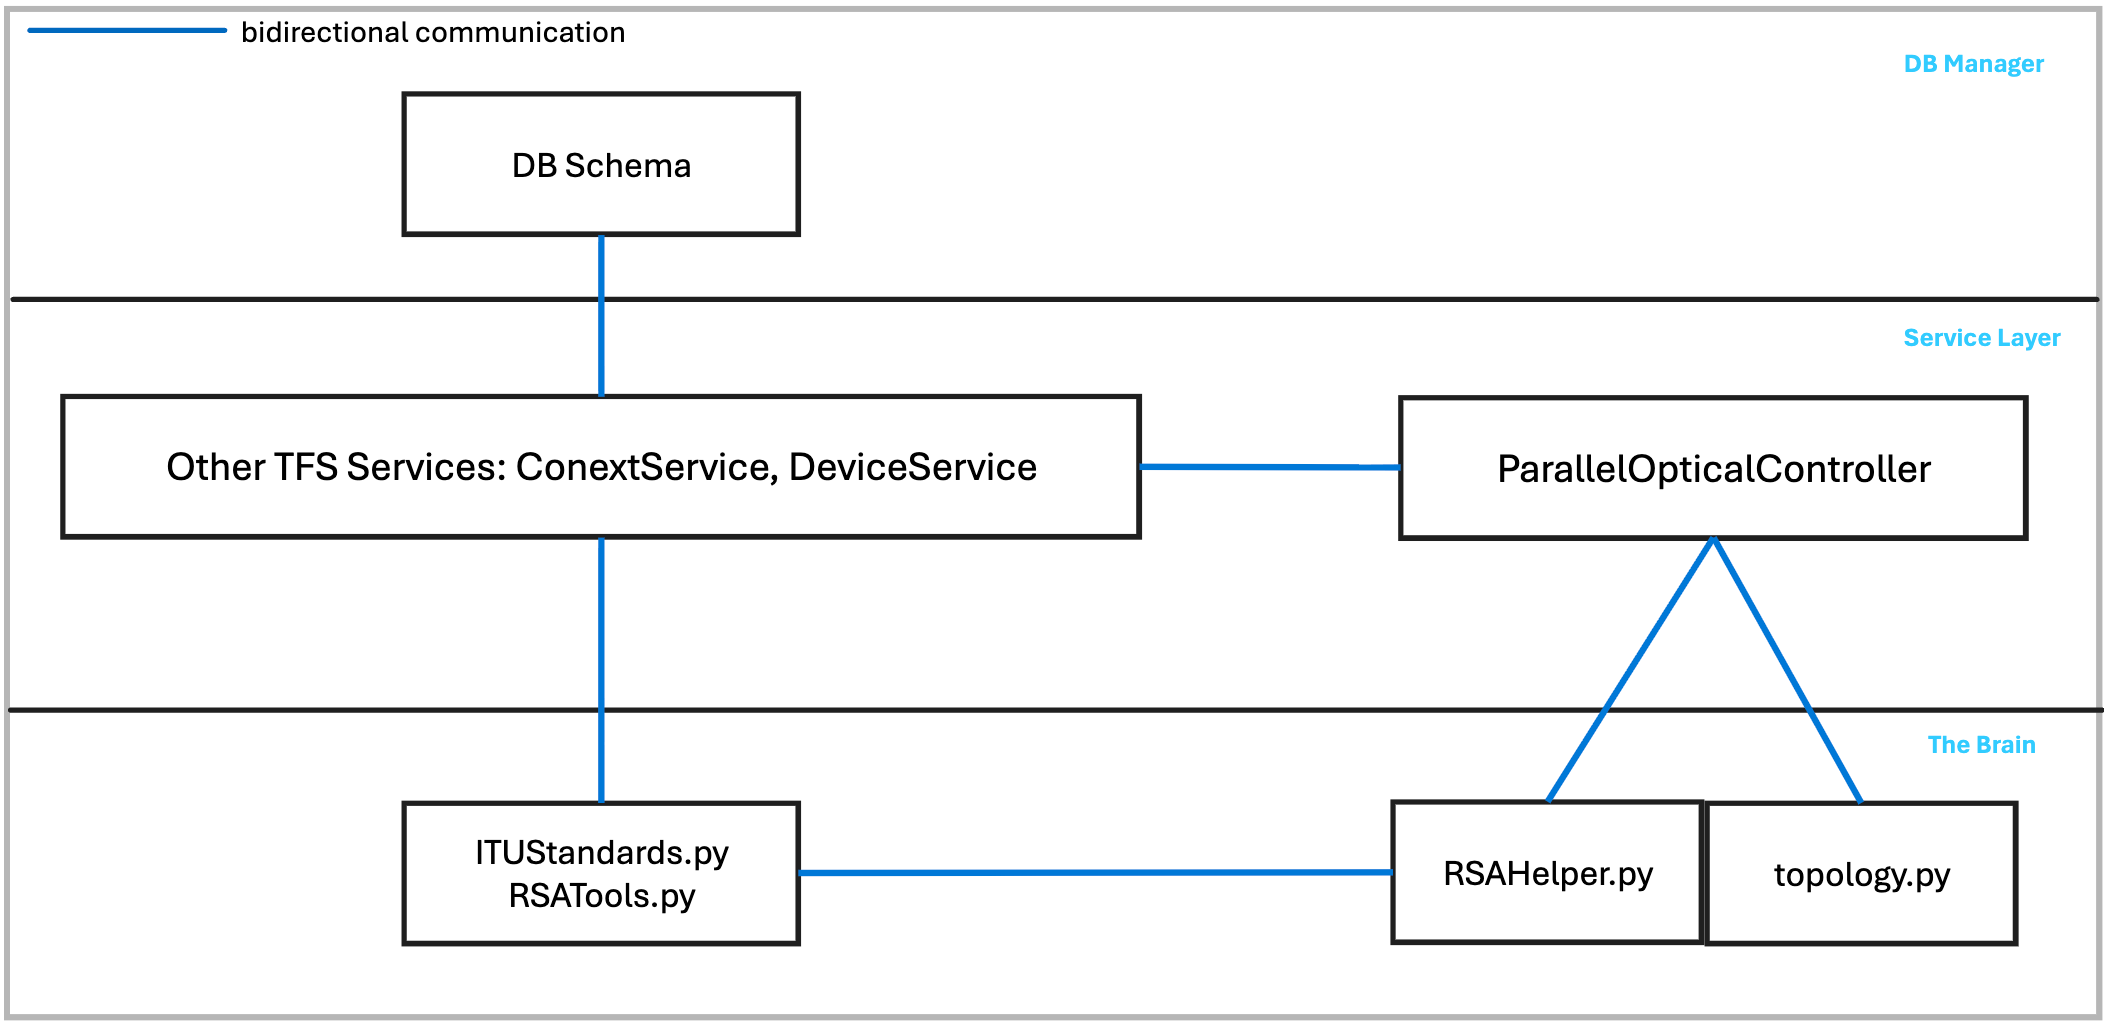
\includegraphics[width=1\textwidth]{poc_service_orchestration.png}
    \caption{Service Architecture of ParallelOpticalController}
    \label{fig:poc_service_orchestration}
\end{figure}
Adhering to official TeraFlowSDN community guidelines, the controller is containerized and orchestrated via MicroK8s. To ensure full interoperability and successfully expose its advanced routing options to the overarching system, the deployment process requires a coordinated restart of specific adjacent microservices (such as the \texttt{DeviceService} and \texttt{ContextService}). A sample automation script used to execute this deployment and synchronization procedure is provided below:
\begin{lstlisting}[language=bash, caption={Deployment of ParallelOpticalController}]
    # On Primary server
    # if you face caching issue, please add --no-cache to the build command
    $ docker build -t localhost:32000/tfs/parallelopticalcontroller:dev -f \ 
    src/parallelopticalcontroller/Dockerfile .

    $ docker push localhost:32000/tfs/parallelopticalcontroller:dev
    
    # if you are building for the first time or have changes in the files names, or ports, or any thing else, update the yaml file and push it again
    $ kubectl apply -f manifests/parallelopticalcontrollerservice.yaml -n tfs
    # otherwise just restart the pod
    $ kubectl rollout restart deployment/parallelopticalcontrollerservice -n tfs
\end{lstlisting}

Once successfully deployed and integrated, the controller assumes an event-driven operational lifecycle. When a new lightpath request is initiated, the TeraFlowSDN core generates a corresponding service request object, which is subsequently exposed to the \texttt{ParallelOpticalController}. However, rather than executing autonomously in the background, the core RSA computation is explicitly triggered by the network operator via the TeraFlowSDN WebUI. This manual trigger initiates a cascade of API interactions and localized function calls across the controller's internal modules (as detailed in the previous helper functions section). The microservice retrieves the real-time context data, formulates the graph, and executes the bitmap-based spatial RSA and slot acquisition protocols. Finally, the controller aggregates the computed data—including the validated physical paths, spatial port mappings, and the final spectrum bitmaps—into a unified, structured response payload. This payload is then transmitted back to the \texttt{WebService}, translating the complex mathematical matrices into an intuitive visual representation for the operator's final review and approval.
\chapter{Testbed Setup and Deployment}
This chapter outlines the physical and logical infrastructure utilized to evaluate the proposed algorithms. It details the installation of the control plane, the configuration of the network emulation environment, and the specific architectural constraints observed to maintain a stable, high-performance testing environment.
\section{Deployment of TeraFlowSDN}
The deployment of the control plane begins by acquiring the TeraFlowSDN source code from the unofficial repository\cite{chafiTFSGit} and following the deployment procedure mentioned in the repository. The official repository can also be followed\cite{tfsRepo} but it excludes \texttt{ParallelOpticalController}. So, for a better deployment-installation of \texttt{Docker, MicroK8s} are recommended from there. However, to optimize server performance during the development and testing of the \texttt{ParallelOpticalController}, a lightweight deployment strategy is highly recommended. By intentionally disabling auxiliary, resource-intensive MicroK8s components—most notably the centralized monitoring subsystem—system overhead is significantly reduced. This targeted reduction ensures that the maximum available CPU and memory resources are strictly dedicated to the controller's core Routing and Spectrum Allocation (RSA) computations.

Beyond resource allocation, establishing a stable testbed requires strict adherence to several critical architectural and operational constraints:
\begin{itemize}
    \item There are documented networking conflicts between MicroK8s and Docker Swarm environments when operated on the same host kernel. Therefore, a distributed, multi-server architecture was adopted. The primary server is dedicated exclusively to the MicroK8s-based TeraFlowSDN deployment, while a secondary, independent server is utilized strictly to host the emulated network devices.
    \item To prevent traffic leakage and avoid interfering with the secondary server's default networking interfaces, a dedicated Docker bridge network must be explicitly provisioned for the device emulation environment.
    \item Post-deployment configuration changes must be heavily restricted. Modifying the hostname of the primary server after initializing MicroK8s and TeraFlowSDN triggers severe state corruption within the Kubernetes cluster, inevitably resulting in data loss. Consequently, server renaming is strictly prohibited once the environment is active, and any unavoidable system reboots demand manual verification of the cluster's recovery state.
    \item For testbeds operating across multiple physical or virtual machines using private IP addressing, explicit routing and unrestricted internal network reachability between the TeraFlowSDN controller node and the device emulation nodes must be validated prior to initializing the control plane.
\end{itemize}
\section{Creating a Virtual Network}
To distribute the computational load and isolate the emulation environment, a secondary server is utilized to host the virtual network infrastructure. This environment is provisioned using Docker, where a dedicated subnet is established and securely bridged to the physical host interface. Subsequently, static IP routing is configured to forward packets directly from the primary TeraFlowSDN server into the secondary server's virtual network. This architectural segregation significantly reduces processing overhead on the primary node and streamlines the NETCONF telemetry and provisioning communication between the SDN controller and the emulated optical devices.

The foundational steps required to initialize this virtual network and establish the inter-server routing are as follows:
\begin{lstlisting}[language=bash, caption={Initialization of the Virtual Network}]
    # Create the docker network in secondary server
    $ sudo docker network create --driver=bridge --ip-range=10.100.0.0/16 \
    --subnet=10.100.0.0/16 -o "com.docker.network.bridge.name=brTFS" netbrTFS

    # Add route in the primary server
    $ sudo ip route add 10.100.0.0/16 via 131.114.54.73

    # Accept packets from the primary server in the secondary server
    $ sudo iptables -I DOCKER-USER -s 131.114.54.72 -d 10.100.0.0/16 -j ACCEPT
\end{lstlisting}
The successful execution of this cross-server routing architecture is heavily dependent on the host operating systems utilized. The procedure outlined above has been validated for an environment utilizing Ubuntu 22.04 on the primary server and Debian Bullseye on the secondary server. However, if Ubuntu 22.04 is deployed on the secondary server, its default network management and strict firewall policies (such as nftables, ufw(is disabled in this scenario) or iptables forwarding rules) necessitate additional configuration steps to permit external traffic into the Docker subnet.

\begin{lstlisting}[language=bash, caption={Ubuntu 22.04 in the secondary server}]
    # Switch iptables to legacy mode
    $ sudo update-alternatives --set iptables /usr/sbin/iptables-legacy

    # Enable IP forwarding (persistent across reboots)
    $ sudo sysctl -w net.ipv4.ip_forward=1
    $ echo "net.ipv4.ip_forward=1" | sudo tee -a /etc/sysctl.conf
    $ sudo sysctl -p

    # Restart Docker (picks up the iptables-legacy switch)
    $ sudo systemctl restart docker

    # Flush Docker's raw PREROUTING DROP rules
    $ sudo nft flush chain ip raw PREROUTING
    $ sudo iptables -t raw -F PREROUTING

    # Ensure the DOCKER-USER chain allows Mascara specifically
    $ sudo iptables -I DOCKER-USER -s 131.114.54.72 -d 10.100.0.0/16 -j ACCEPT

    # Force the kernel to allow forwarding to your specific bridge
    $ sudo sysctl -w net.ipv4.ip_forward=1
    $ sudo iptables -I FORWARD -o brTFS -j ACCEPT
    $ sudo iptables -I FORWARD -i brTFS -j ACCEPT
\end{lstlisting}
Each time a container is up or restarted, the following commands must be executed again. Following the execution of these network configurations, manual verification is mandatory to confirm end-to-end reachability across the testbed. System administrators must ensure that the primary server can successfully route packets directly to the isolated Docker containers hosted on the secondary server. This validation is efficiently achieved via a standard ICMP echo request directed at a running container's designated IP address.
\section{Emulated Devices}
The physical optical layer of the testbed is simulated using Docker and Docker Swarm containerization, allowing for the deployment of a highly scalable, virtualized network topology. The emulation environment specifically provisions two fundamental classes of optical equipment: Muxponders (acting as the optical terminal endpoints) and Reconfigurable Optical Add-Drop Multiplexers (ROADMs). The underlying container images for these emulators leverage established academic repositories initially developed by professor Alessio and Andrea, which provide a robust and highly configurable baseline for optical device simulation. Upon initialization, the default operational states of these emulated devices are dynamically updated using configuration files injected directly from the SDN controller via the NETCONF protocol. These configurations are formatted as XML payloads and rigorously adhere to standardized OpenConfig and OpenROADM YANG data models.
\section{An Example Topology Deployment}
Building upon the previously established configuration, this section provides a comprehensive walkthrough for instantiating a functional linear optical topology within the TeraFlowSDN environment. The deployment process requires the execution of specific automation scripts to generate the emulated hardware, followed by the ingestion of structured JSON descriptor files into the SDN control plane. This procedure assumes that the secondary server's virtual network has been successfully provisioned and that cross-server packet routing is fully operational, as detailed in the preceding sections.

The structured deployment protocol is executed as follows:
\begin{enumerate}
    \item \textbf{Device Emulation Initialization} \vspace{0.2cm} \\Access the secondary server and execute the \texttt{allGenerate.sh} script (located at \texttt{/test/generic/} within the project repository \cite{chafiTFSGit}) to deploy the containerized optical devices\footnote{- Administrator (sudo) privileges are required for this execution.}. Once the Docker containers are actively running, it is highly recommended to verify network reachability by executing a standard ping request from the primary server to the newly created emulated devices.
    \item \textbf{Service Verification} \vspace{0.2cm} \\On the primary server, launch a terminal session and execute the following command to confirm that all required TeraFlowSDN microservices are in an active and healthy state: \texttt{"watch -n 1 kubectl get all --all-namespaces"}
    \item \textbf{Base Context Initialization} \vspace{0.2cm} \\Navigate to the TeraFlowSDN WebUI (accessible via the \texttt{/webui} web endpoint) and upload the \texttt{adminContext.json} descriptor file. This crucial initialization file establishes the default administrative context and the foundational baseline topology\footnote{- The default behavior of teraflowSDN is to add every resource within admin context and topology. If additional contexts and topologies are to be created, they must be followed after the default one.}, which serve as mandatory structural prerequisites for all subsequent SDN operations.
    \item \textbf{Base Context Initialization} \vspace{0.2cm} \\Following the base initialization, upload the specific device registration descriptor (\texttt{generic\_adminContext.json}, located at \texttt{/test/generic/}) via the WebUI. This process systematically parses the device telemetry and formally registers the emulated physical hardware with the central context database.
    \item \textbf{Topology Formulation} \vspace{0.2cm} \\To construct the final logical network, upload the topology descriptor (\texttt{linea\_si\\-ngle.json}) within the same repository. This configuration file instructs the control plane to map the recently onboarded optical devices into a distinct operational context and systematically establishes the specific physical links connecting them.
\end{enumerate}

\subsection*{\small Visualization and Verification}
Upon the successful sequential ingestion of these JSON descriptors, the network operator can select the newly established context from the WebUI dropdown menu. This action triggers the interface to query the database and render a comprehensive visual representation of the active linear topology, confirming the successful synchronization between the emulated hardware and the SDN control plane.

\begin{figure}[htbp]
    \centering
    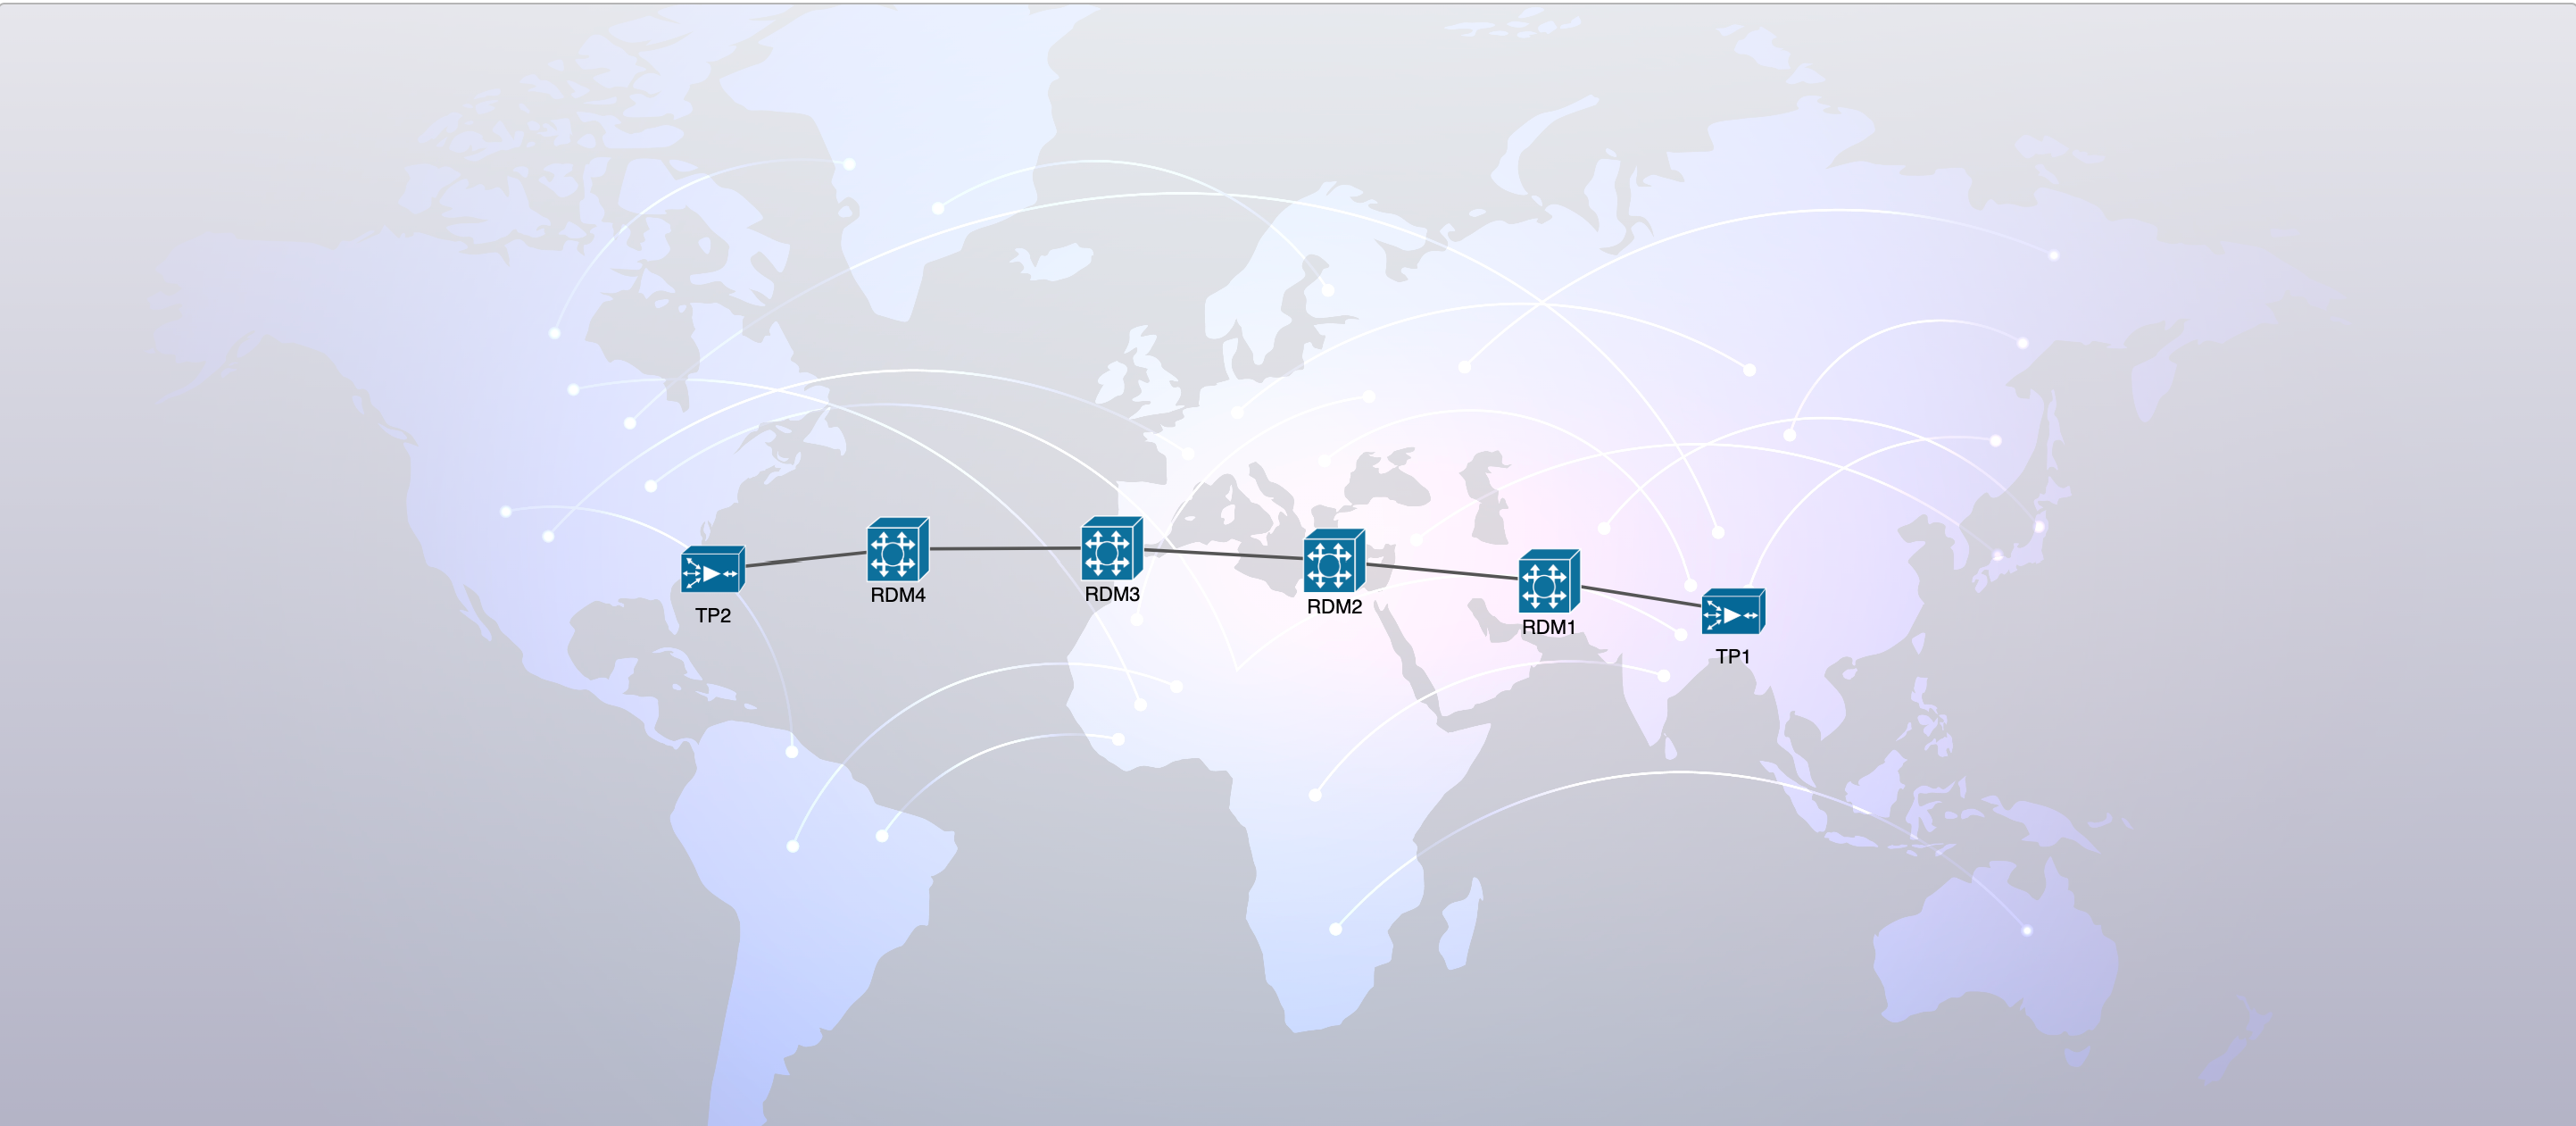
\includegraphics[width=0.8\textwidth]{linear_single_topo.png}
    \caption{An example topology in TeraflowSDN}
    \label{fig:linear_single_topo}
\end{figure}
\chapter{Results and Evaluation}
This chapter presents a comprehensive performance evaluation and functional validation of the proposed Routing and Spectrum Allocation (RSA) framework. To substantiate the theoretical claims established in preceding chapters, the newly integrated \texttt{ParallelOpticalController} is rigorously tested within the TeraFlowSDN ecosystem across a variety of multi-fiber reference topologies. The subsequent sections provide an in-depth assessment of the system's operational success, systematically analyzing its computational performance and algorithmic efficiency. Furthermore, this chapter details network throughput metrics, conducts a statistical analysis of path blocking probabilities, and presents a direct comparative evaluation against traditional RSA approaches to explicitly benchmark the operational advantages of the proposed bitwise spectrum allocation methodology.
\section{Evaluation Methodology \& Test Scenarios}
To rigorously evaluate the performance and resilience of the proposed \texttt{ParallelOpti-\\calController}, a comprehensive series of test scenarios were executed within the established Docker-based emulation environment. The evaluation methodology focuses on injecting dynamic optical intents (lightpath requests) into the TeraFlowSDN control plane and systematically monitoring the system's computational and operational responses across multiple performance metrics.

The test scenarios were designed to evaluate the system across various network architectures, with a specific focus on multi-directed graphs where optical nodes (e.g., Muxponders and ROADMs) are connected via multiple parallel fiber links. The primary objectives of these evaluations are threefold:
\begin{enumerate}
    \item To validate the functional correctness of the driver-level device telemetry extraction.
    \item To measure the computational latency and efficiency of the path discovery and bitmap-based RSA algorithms.
    \item To statistically analyze network throughput and path blocking probabilities under varying, simulated traffic loads.
\end{enumerate}
To ensure a robust evaluation, testing was conducted across four distinct network topologies, each exhibiting varying degrees of node density and meshing. To explicitly demonstrate the controller's multi-fiber capabilities, each topology was evaluated in two configurations: a baseline "Single" configuration (one fiber per link) and a "Parallel" configuration (multiple fibers per link). The topologies utilized are as follows:
\begin{itemize}
    \item \textbf{Linear Topology:} A standard point-to-point chain comprising 6 nodes. The single version has 5 links and the parallel has 13 links.
          \begin{figure}[htbp]
              \centering
              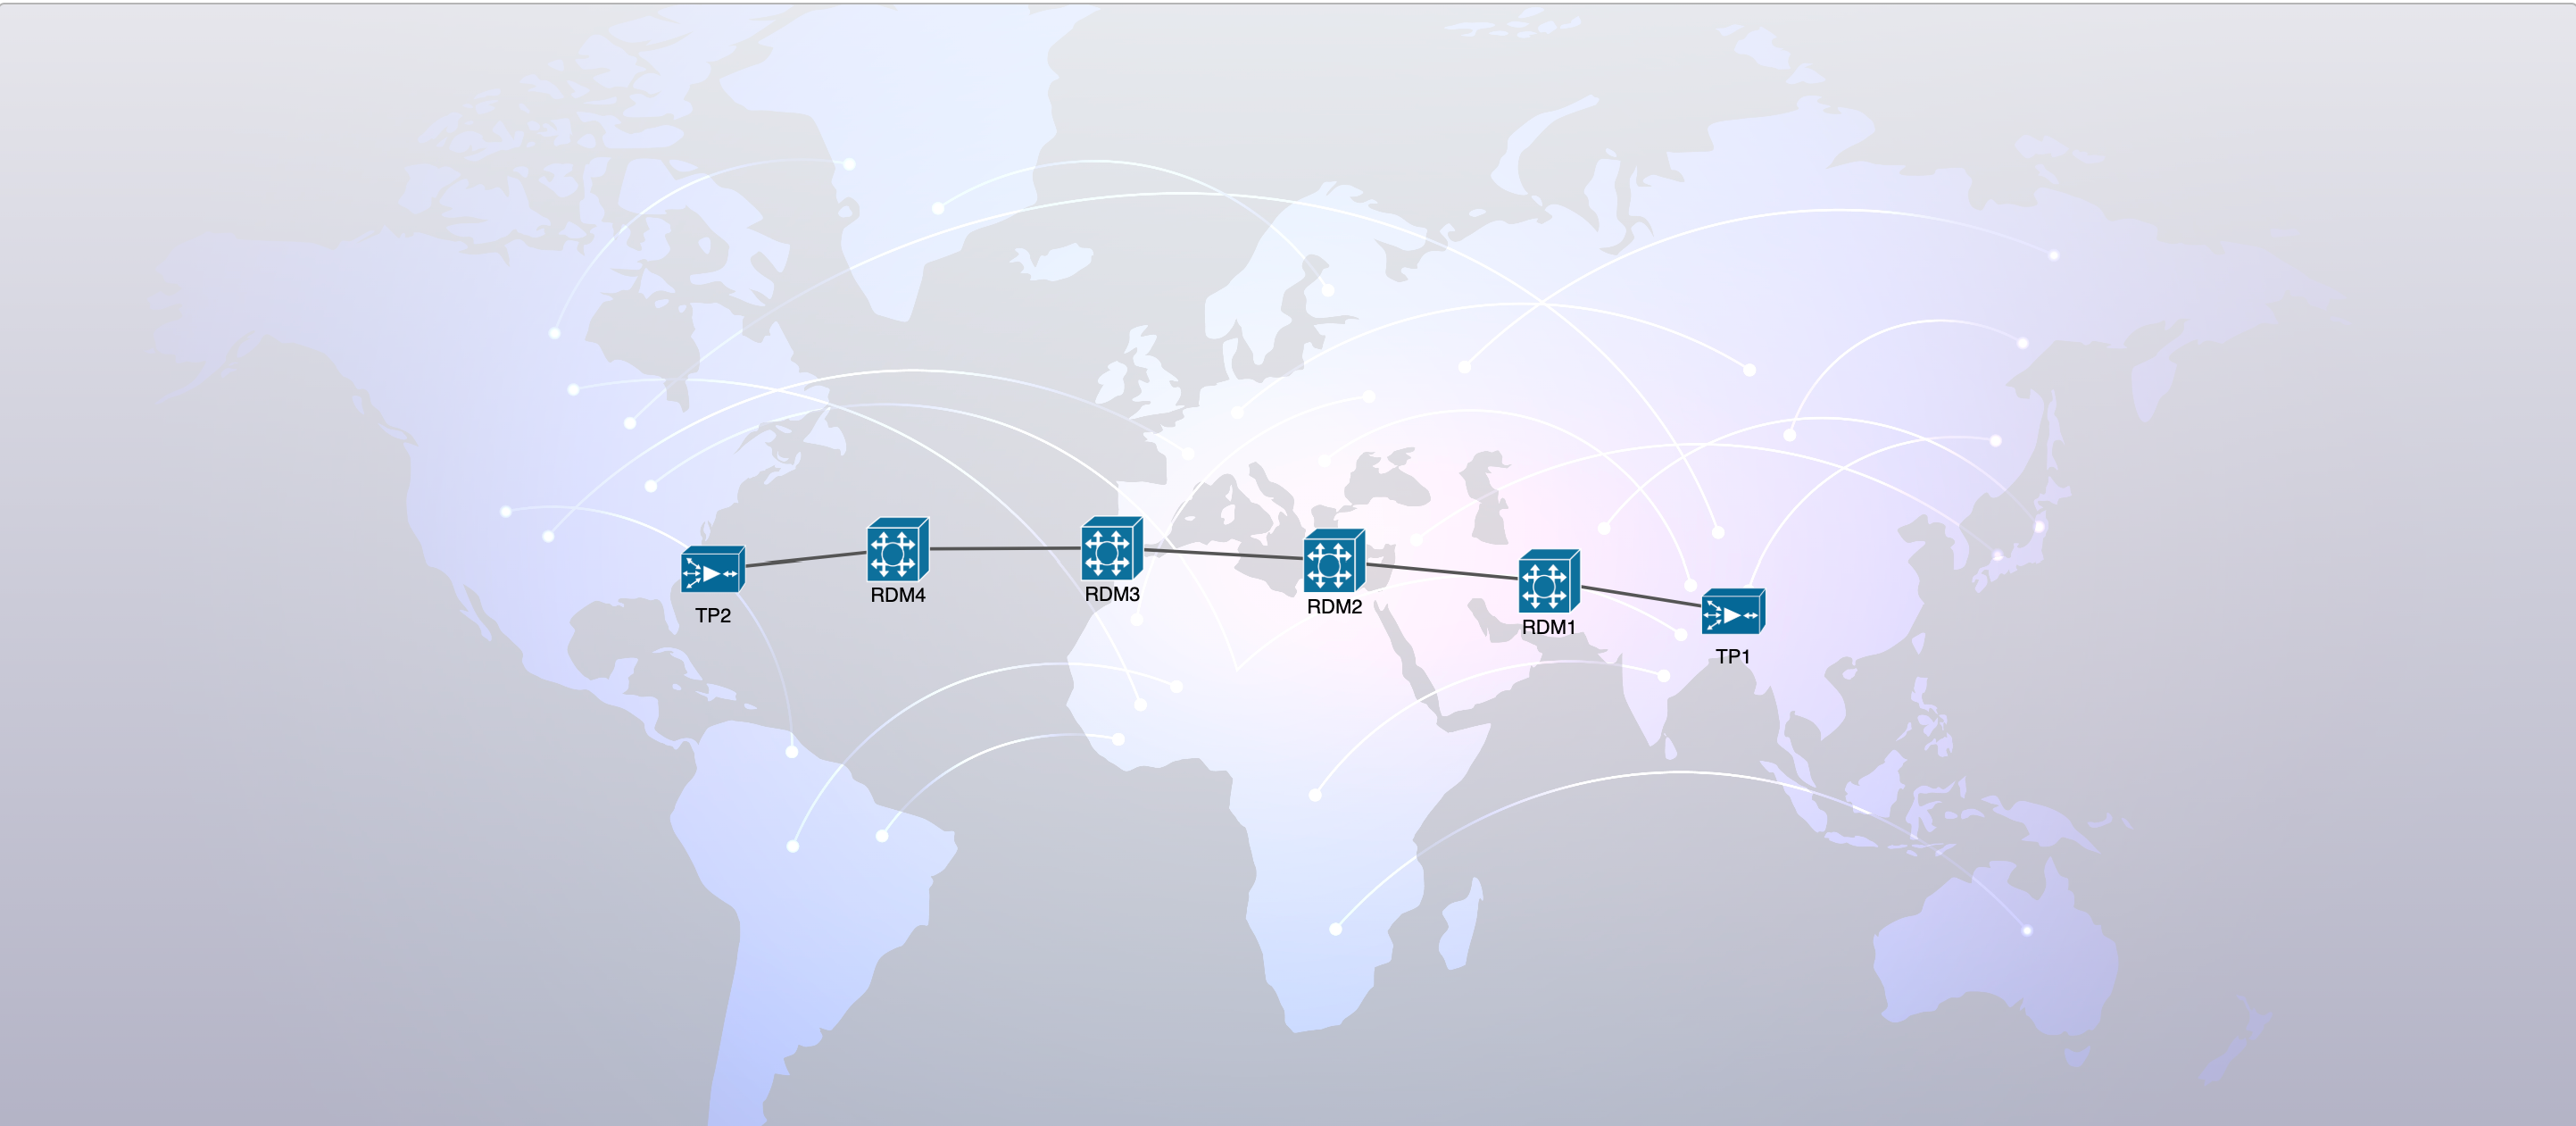
\includegraphics[width=1\textwidth]{linear_single_topo.png}
              \caption{Linear Topology(no parallel links)}
          \end{figure}
    \item \textbf{Butterfly Topology:} A foundational meshed architecture comprising 10 nodes. The single version has 10 links and the parallel has 26 links.
          \begin{figure}[htbp]
              \centering
              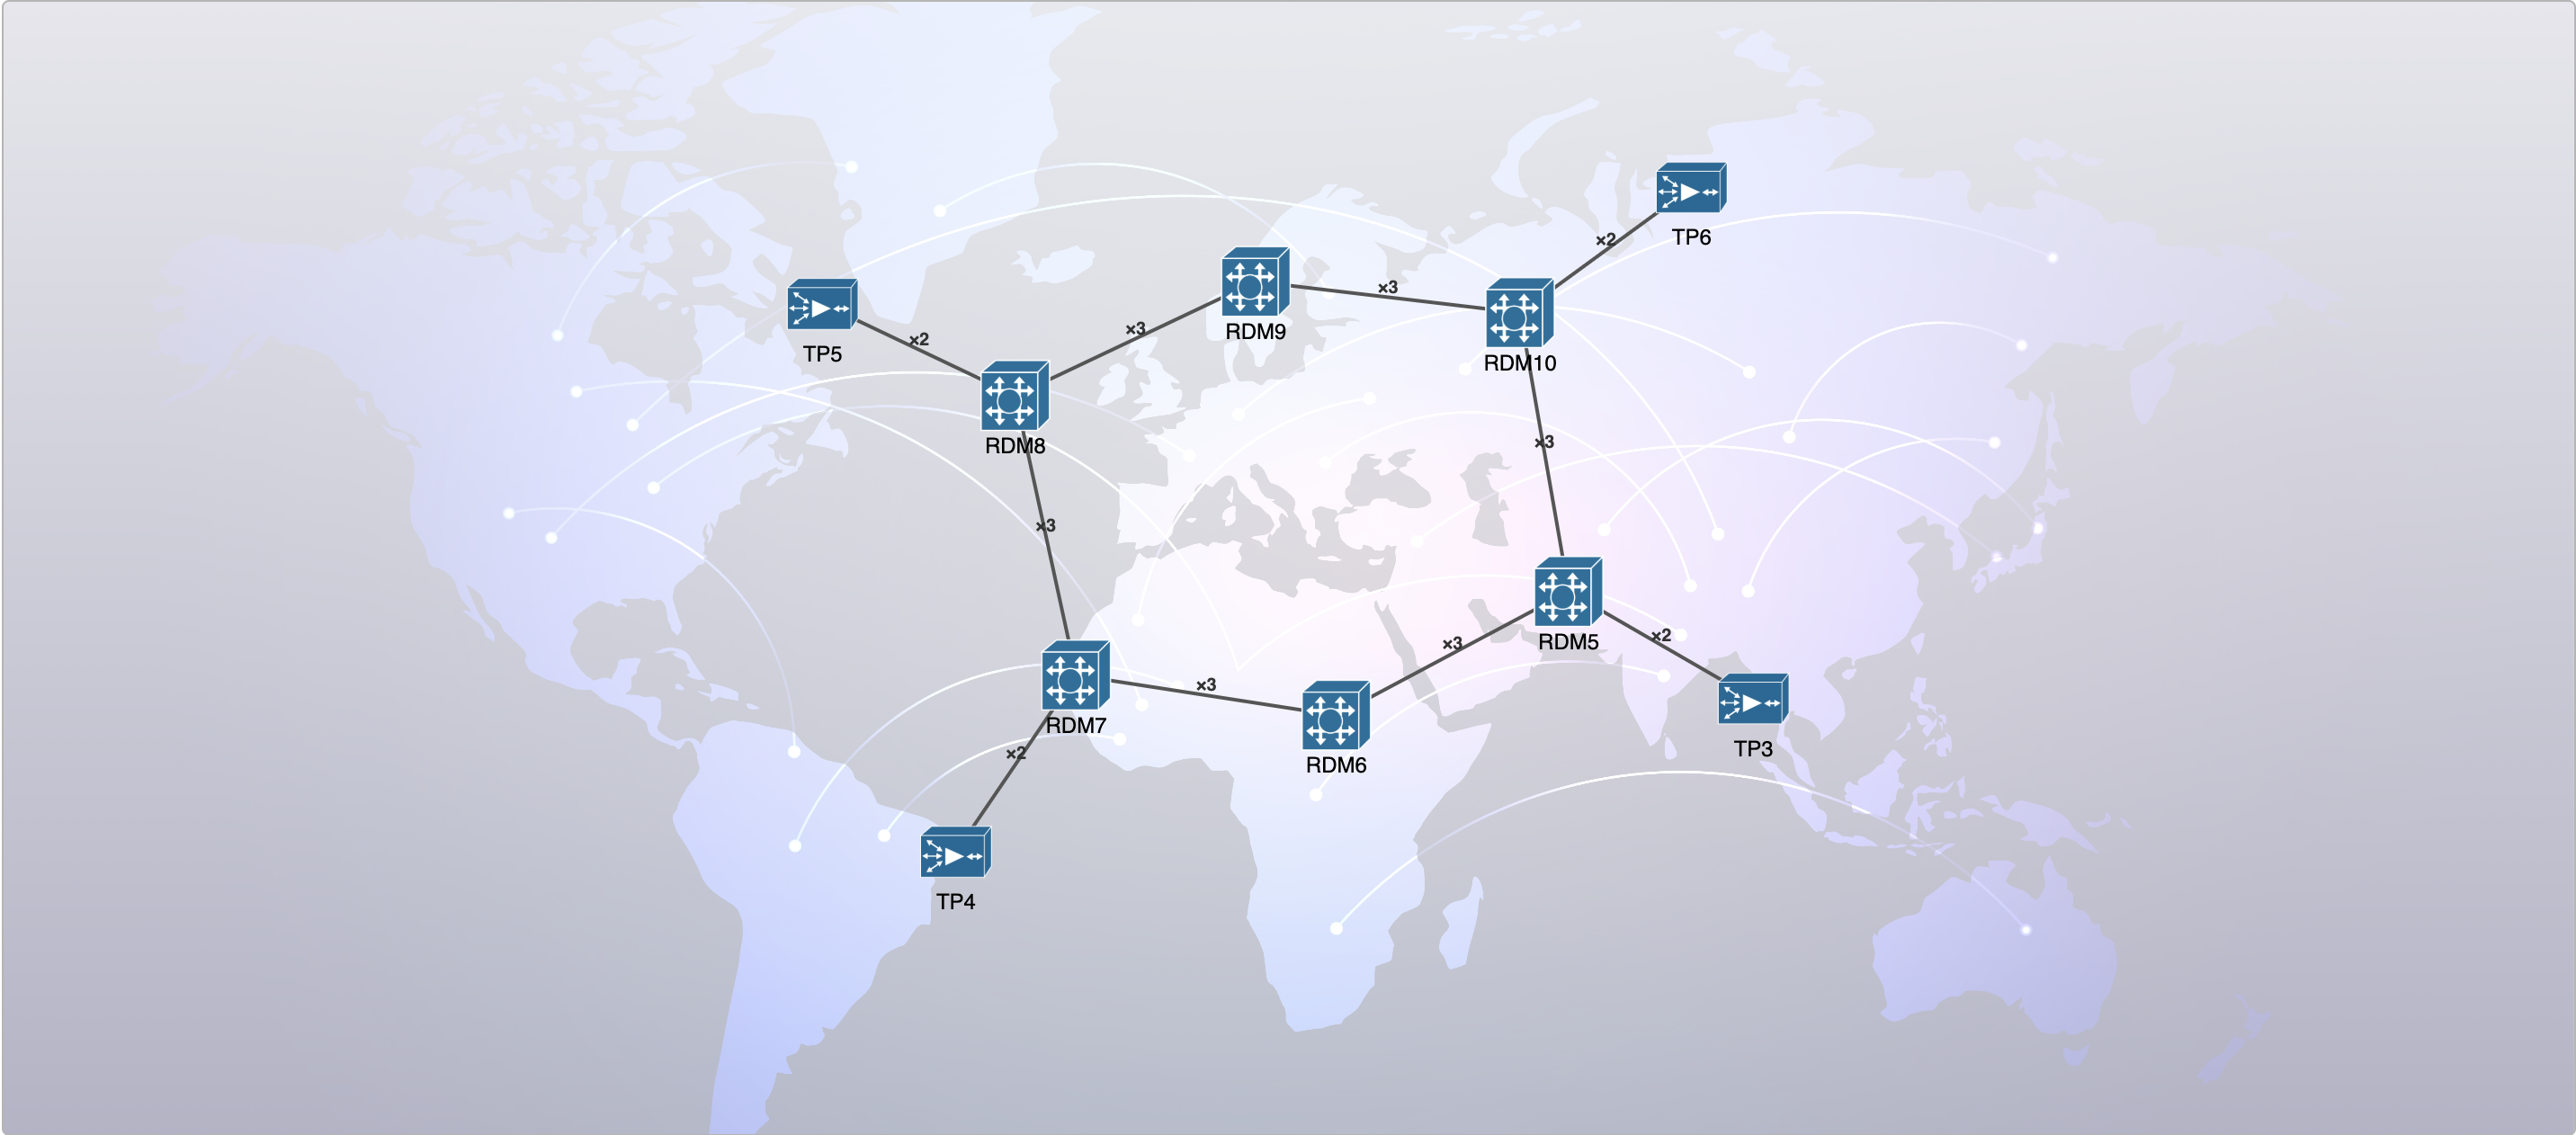
\includegraphics[width=1\textwidth]{butterfly_parallel.png}
              \caption{Butterfly Topology(with parallel links)}
              \label{fig:butterfly_parallel}
          \end{figure}
    \item \textbf{NSFNet Topology:} A well-known reference model of the National Science Foundation Network comprising 23 nodes. The single version has 33 links and the parallel has 60 links.
          \begin{figure}[htbp]
              \centering
              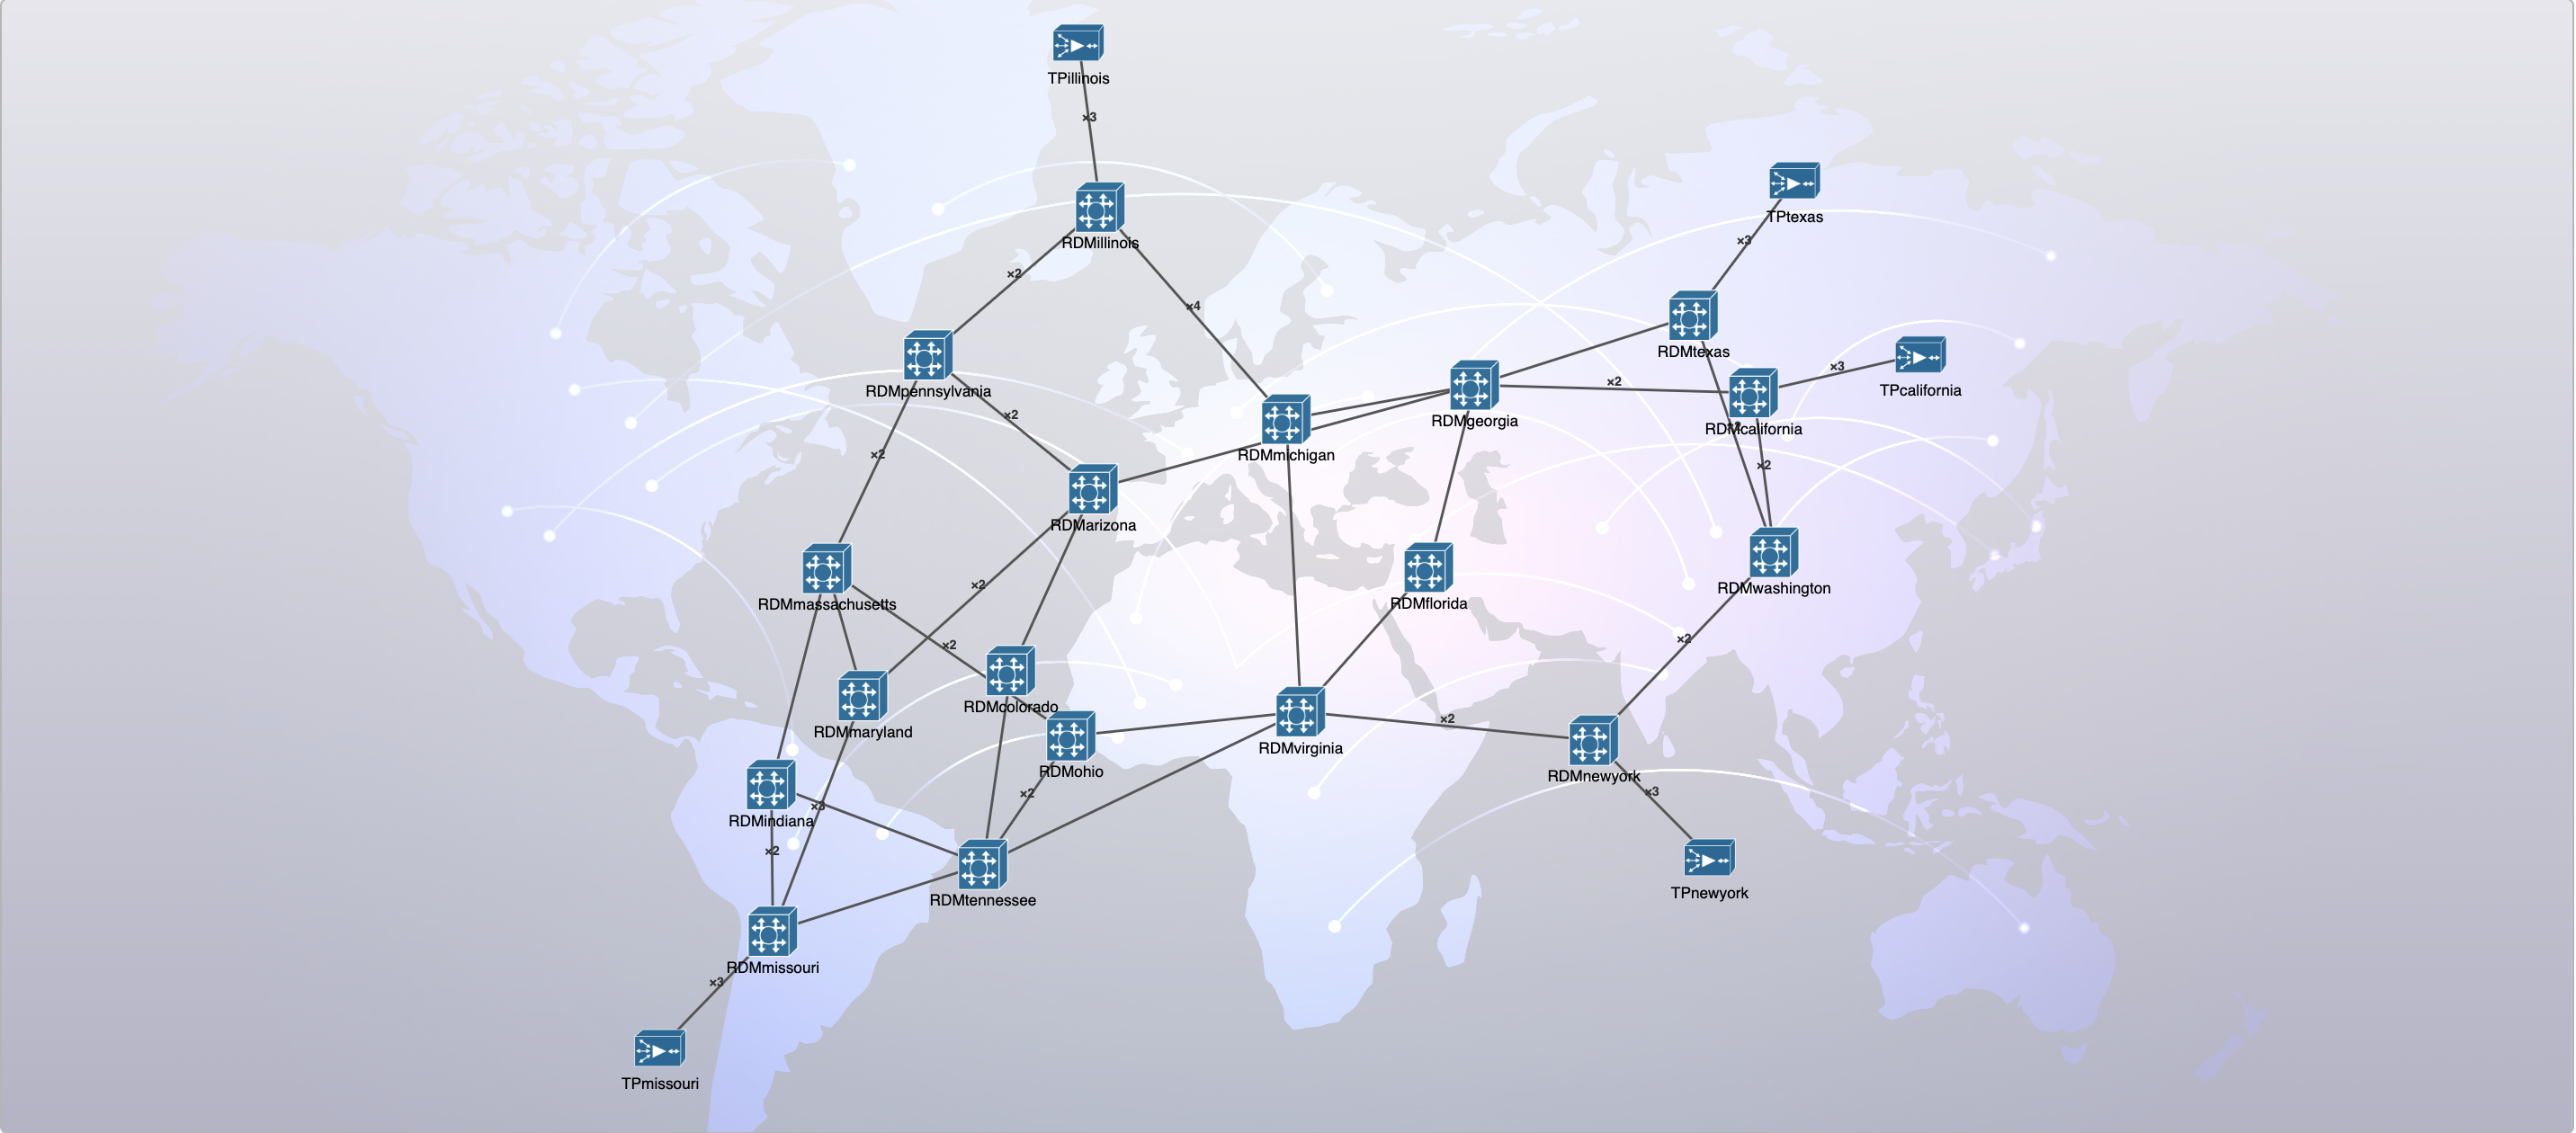
\includegraphics[width=1\textwidth]{nsf_parallel.png}
              \caption{NSFNet Topology(with parallel links)}
              \label{fig:nsf_parallel}
          \end{figure}
    \item \textbf{Pan-European (PANEU) Topology:} A highly dense, complex reference model comprising 37 nodes. The single version has 62 links and the parallel has 105 links.
          \begin{figure}[htbp]
              \centering
              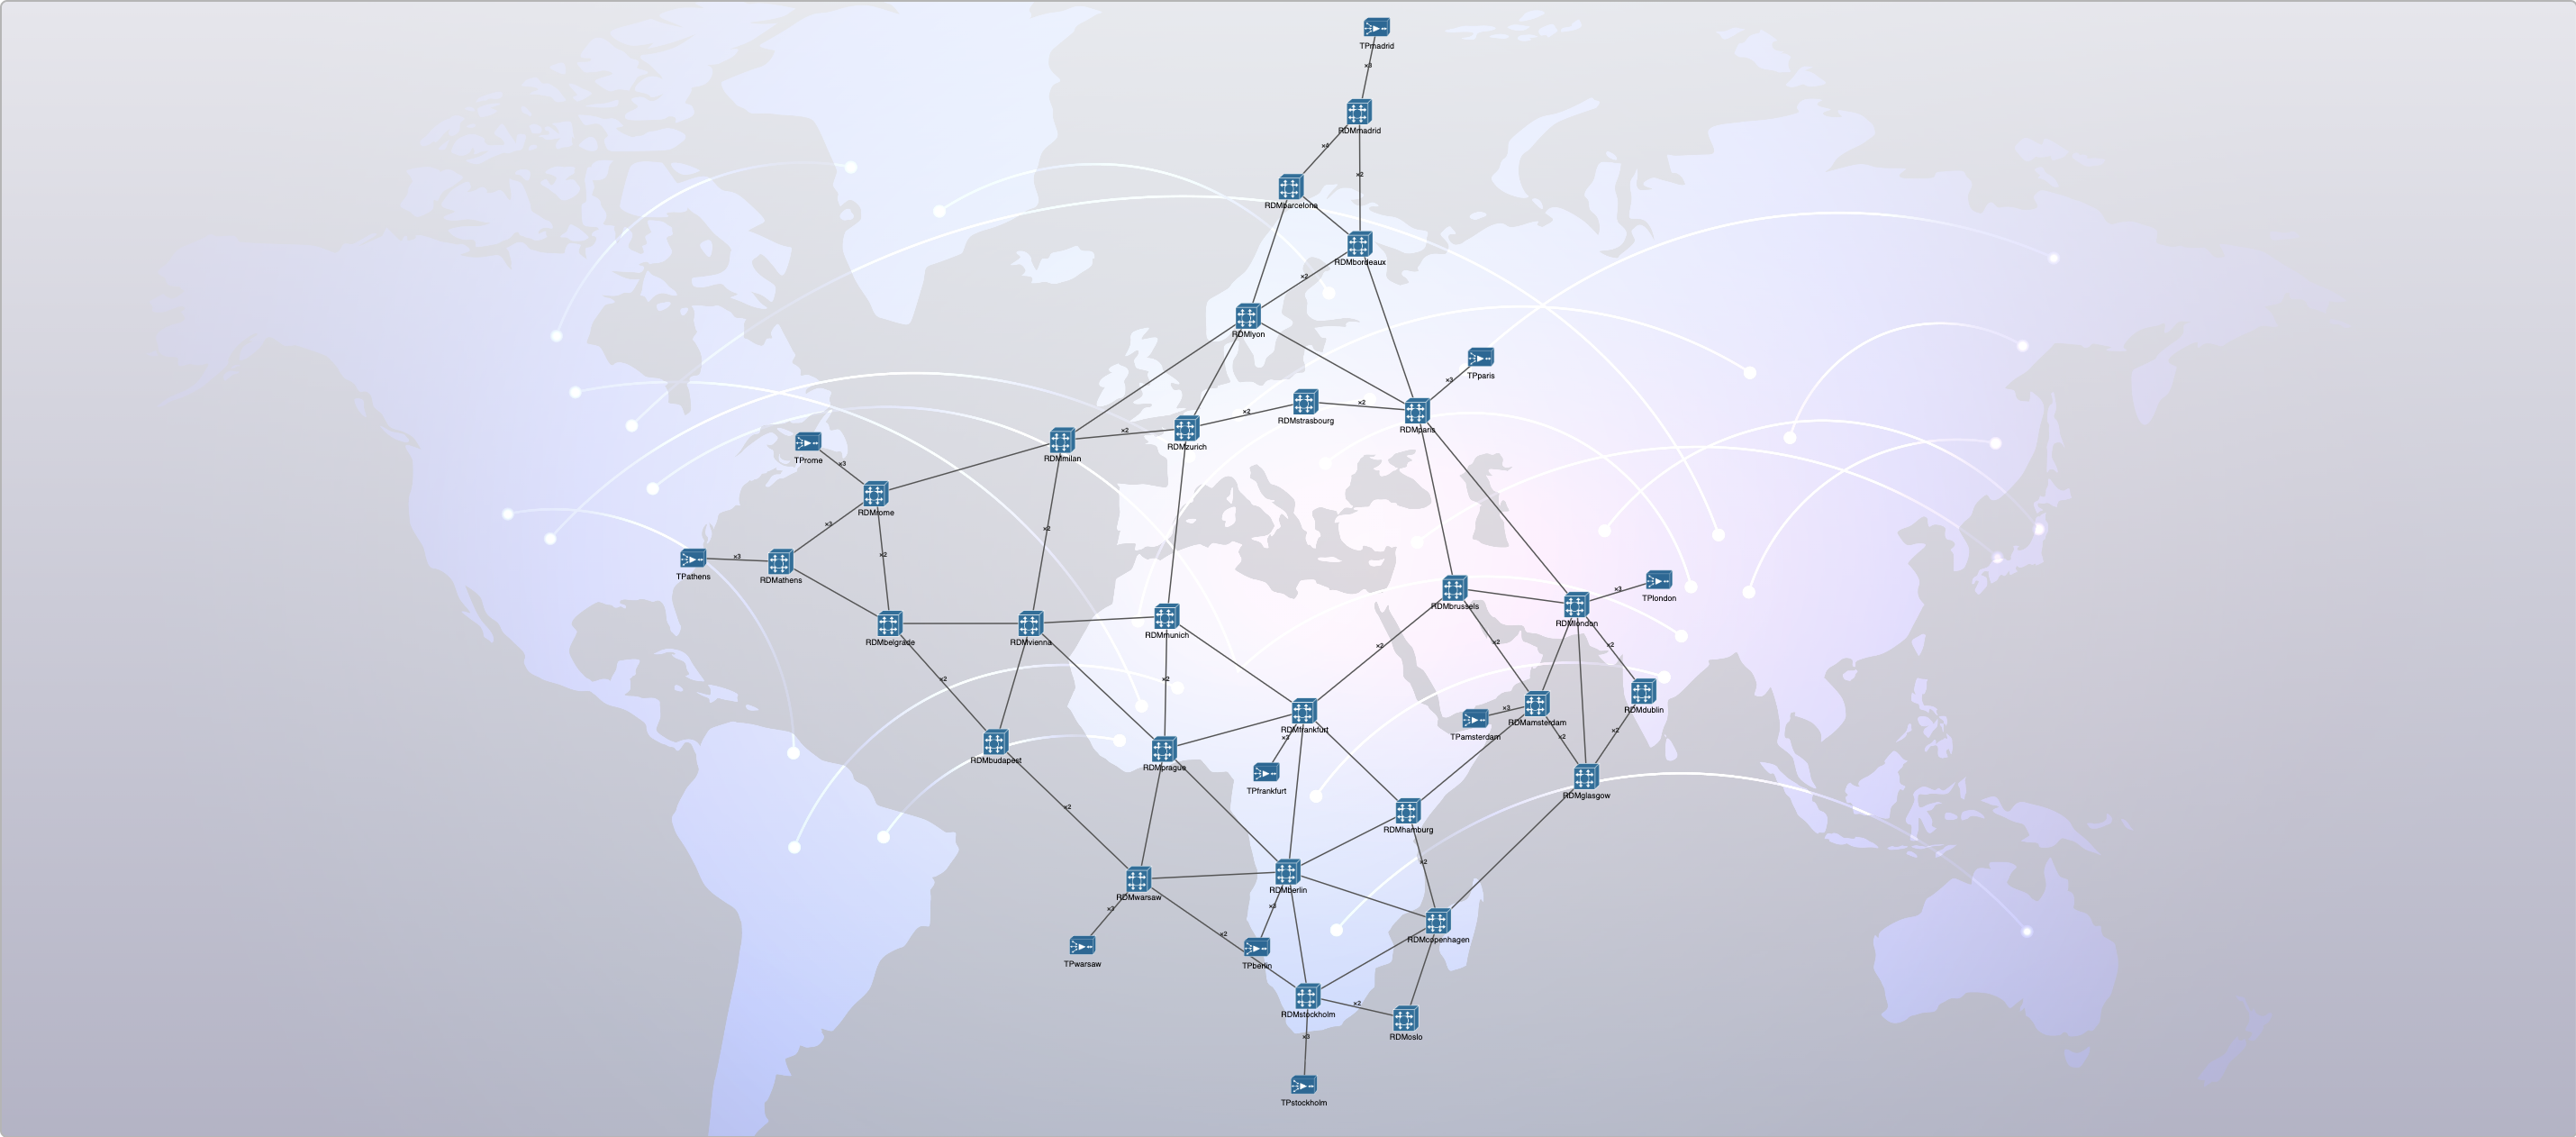
\includegraphics[width=1\textwidth]{paneu_parallel.png}
              \caption{PANEU Topology(with parallel links)}
              \label{fig:paneu_parallel}
          \end{figure}
\end{itemize}
While computational performance and functional correctness were assessed across all four topologies, the subsequent statistical analysis—focusing on path blocking and spectrum utilization under heavy traffic loads—was exclusively focused on the more complex NSFNet and PANEU models, as they better represent the scale and behavior of real-world wide-area optical networks.
\section{Functional Validation}
Prior to evaluating quantitative performance metrics, it is imperative to establish the foundational functional correctness of the integrated system. This validation was achieved by systematically corroborating the internal backend execution logs with the topological and spectral state rendered on the enhanced TeraFlowSDN Web User Interface (WebUI). This section demonstrates the operational success of each core feature engineered for the \texttt{ParallelOpticalController} microservice. The validation process entails a detailed, step-by-step examination of the system's operational lifecycle. Specifically, it visualizes the accurate extraction of hardware telemetry, the precise mapping of flexible-grid frequency slots, the generation of spectrum allocation matrices (RSA tables), and the successful execution of spatial comparisons across parallel multi-fiber links.

To definitively substantiate these visual interface elements, direct excerpts from the controller's backend execution logs are presented alongside them. This cross-referencing ensures that the visual representation accurately reflects the underlying database state, thereby confirming that the bitmap-based mathematical computations align perfectly with the theoretical algorithmic design.

\subsection*{\small Device info extraction}
The following WebUI visualization confirms that these extracted, granular parameters are successfully propagated through the \texttt{ContextService} and accurately rendered on the operator dashboard.
\begin{figure}[htbp]
    \centering
    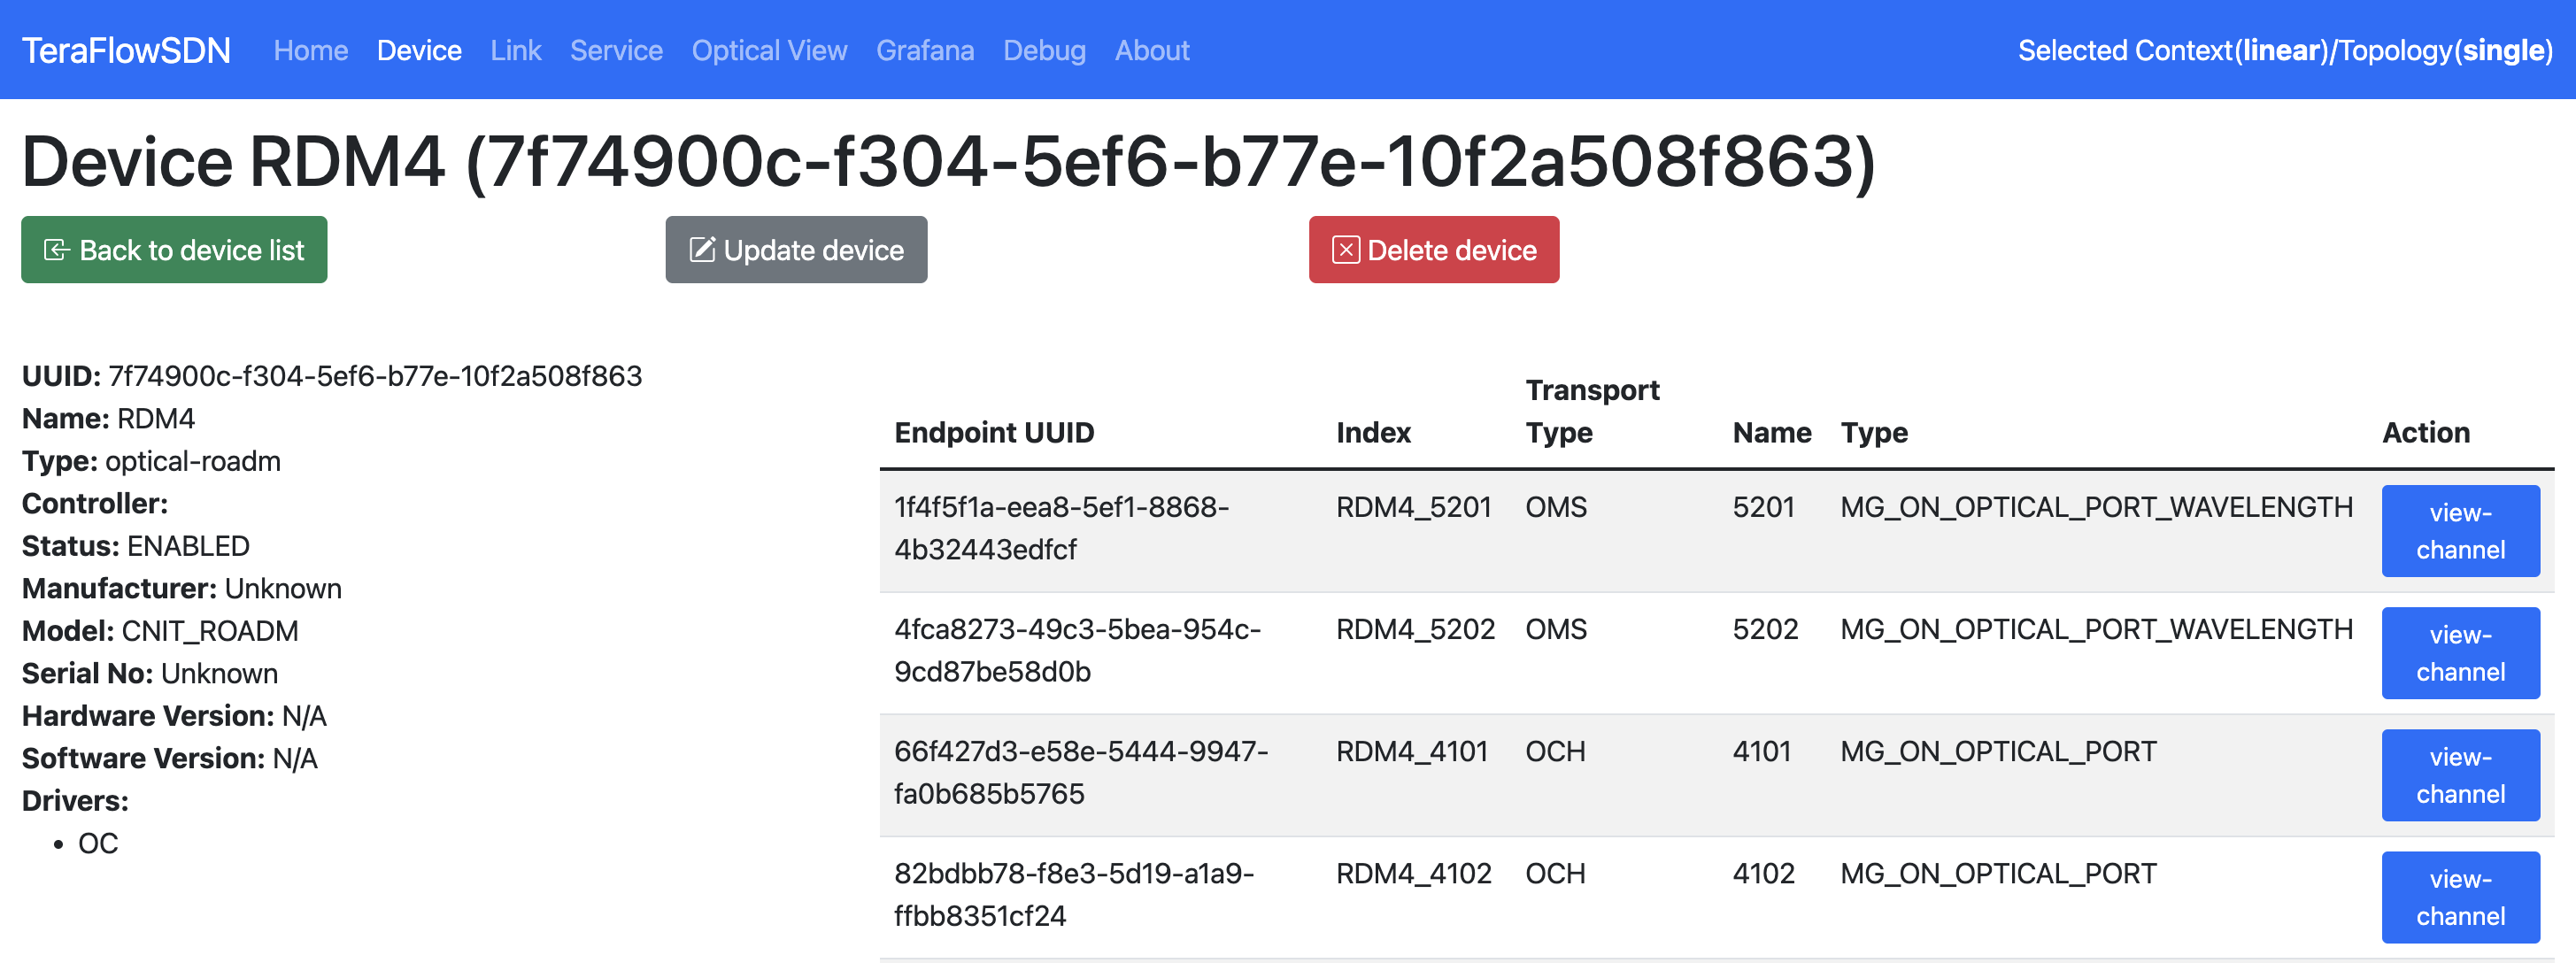
\includegraphics[width=0.8\textwidth]{web_view_device_info.png}
    \caption{Web view of device info}
    \label{fig:web_view_device_info}
\end{figure}

Correspondingly, the execution log demonstrates the enhancements implemented within the \texttt{OCDriver} to accurately extract complex optical device telemetry. Crucially, this output validates the architectural claim that the extraction methodology dynamically adapts based on the specific hardware vendor and device model identified during initialization.

\begin{figure}[htbp]
    \centering
    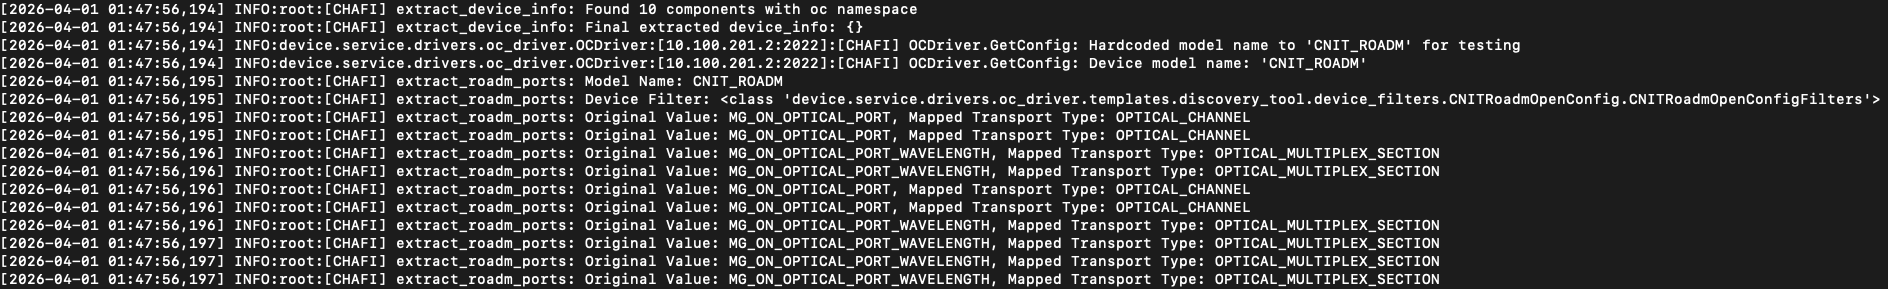
\includegraphics[width=1\textwidth]{device_info_extraction.png}
    \caption{Device info extraction using OCDriver}
    \label{fig:device_info_extraction}
\end{figure}

\begin{figure}[htbp]
    \centering
    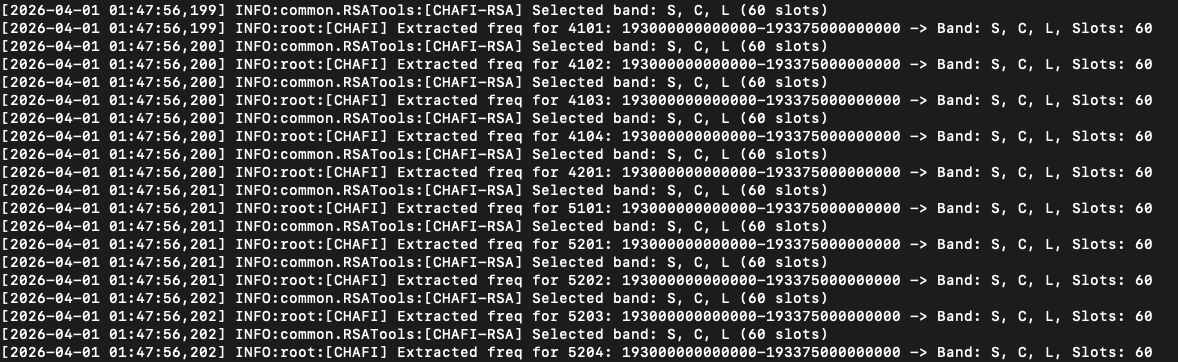
\includegraphics[width=1\textwidth]{frequency_mapping_roadm_ports.png}
    \caption{Frequency mapping of the device endpoints}
    \label{fig:frequency_mapping_roadm_ports}
\end{figure}

\begin{figure}[htbp]
    \centering
    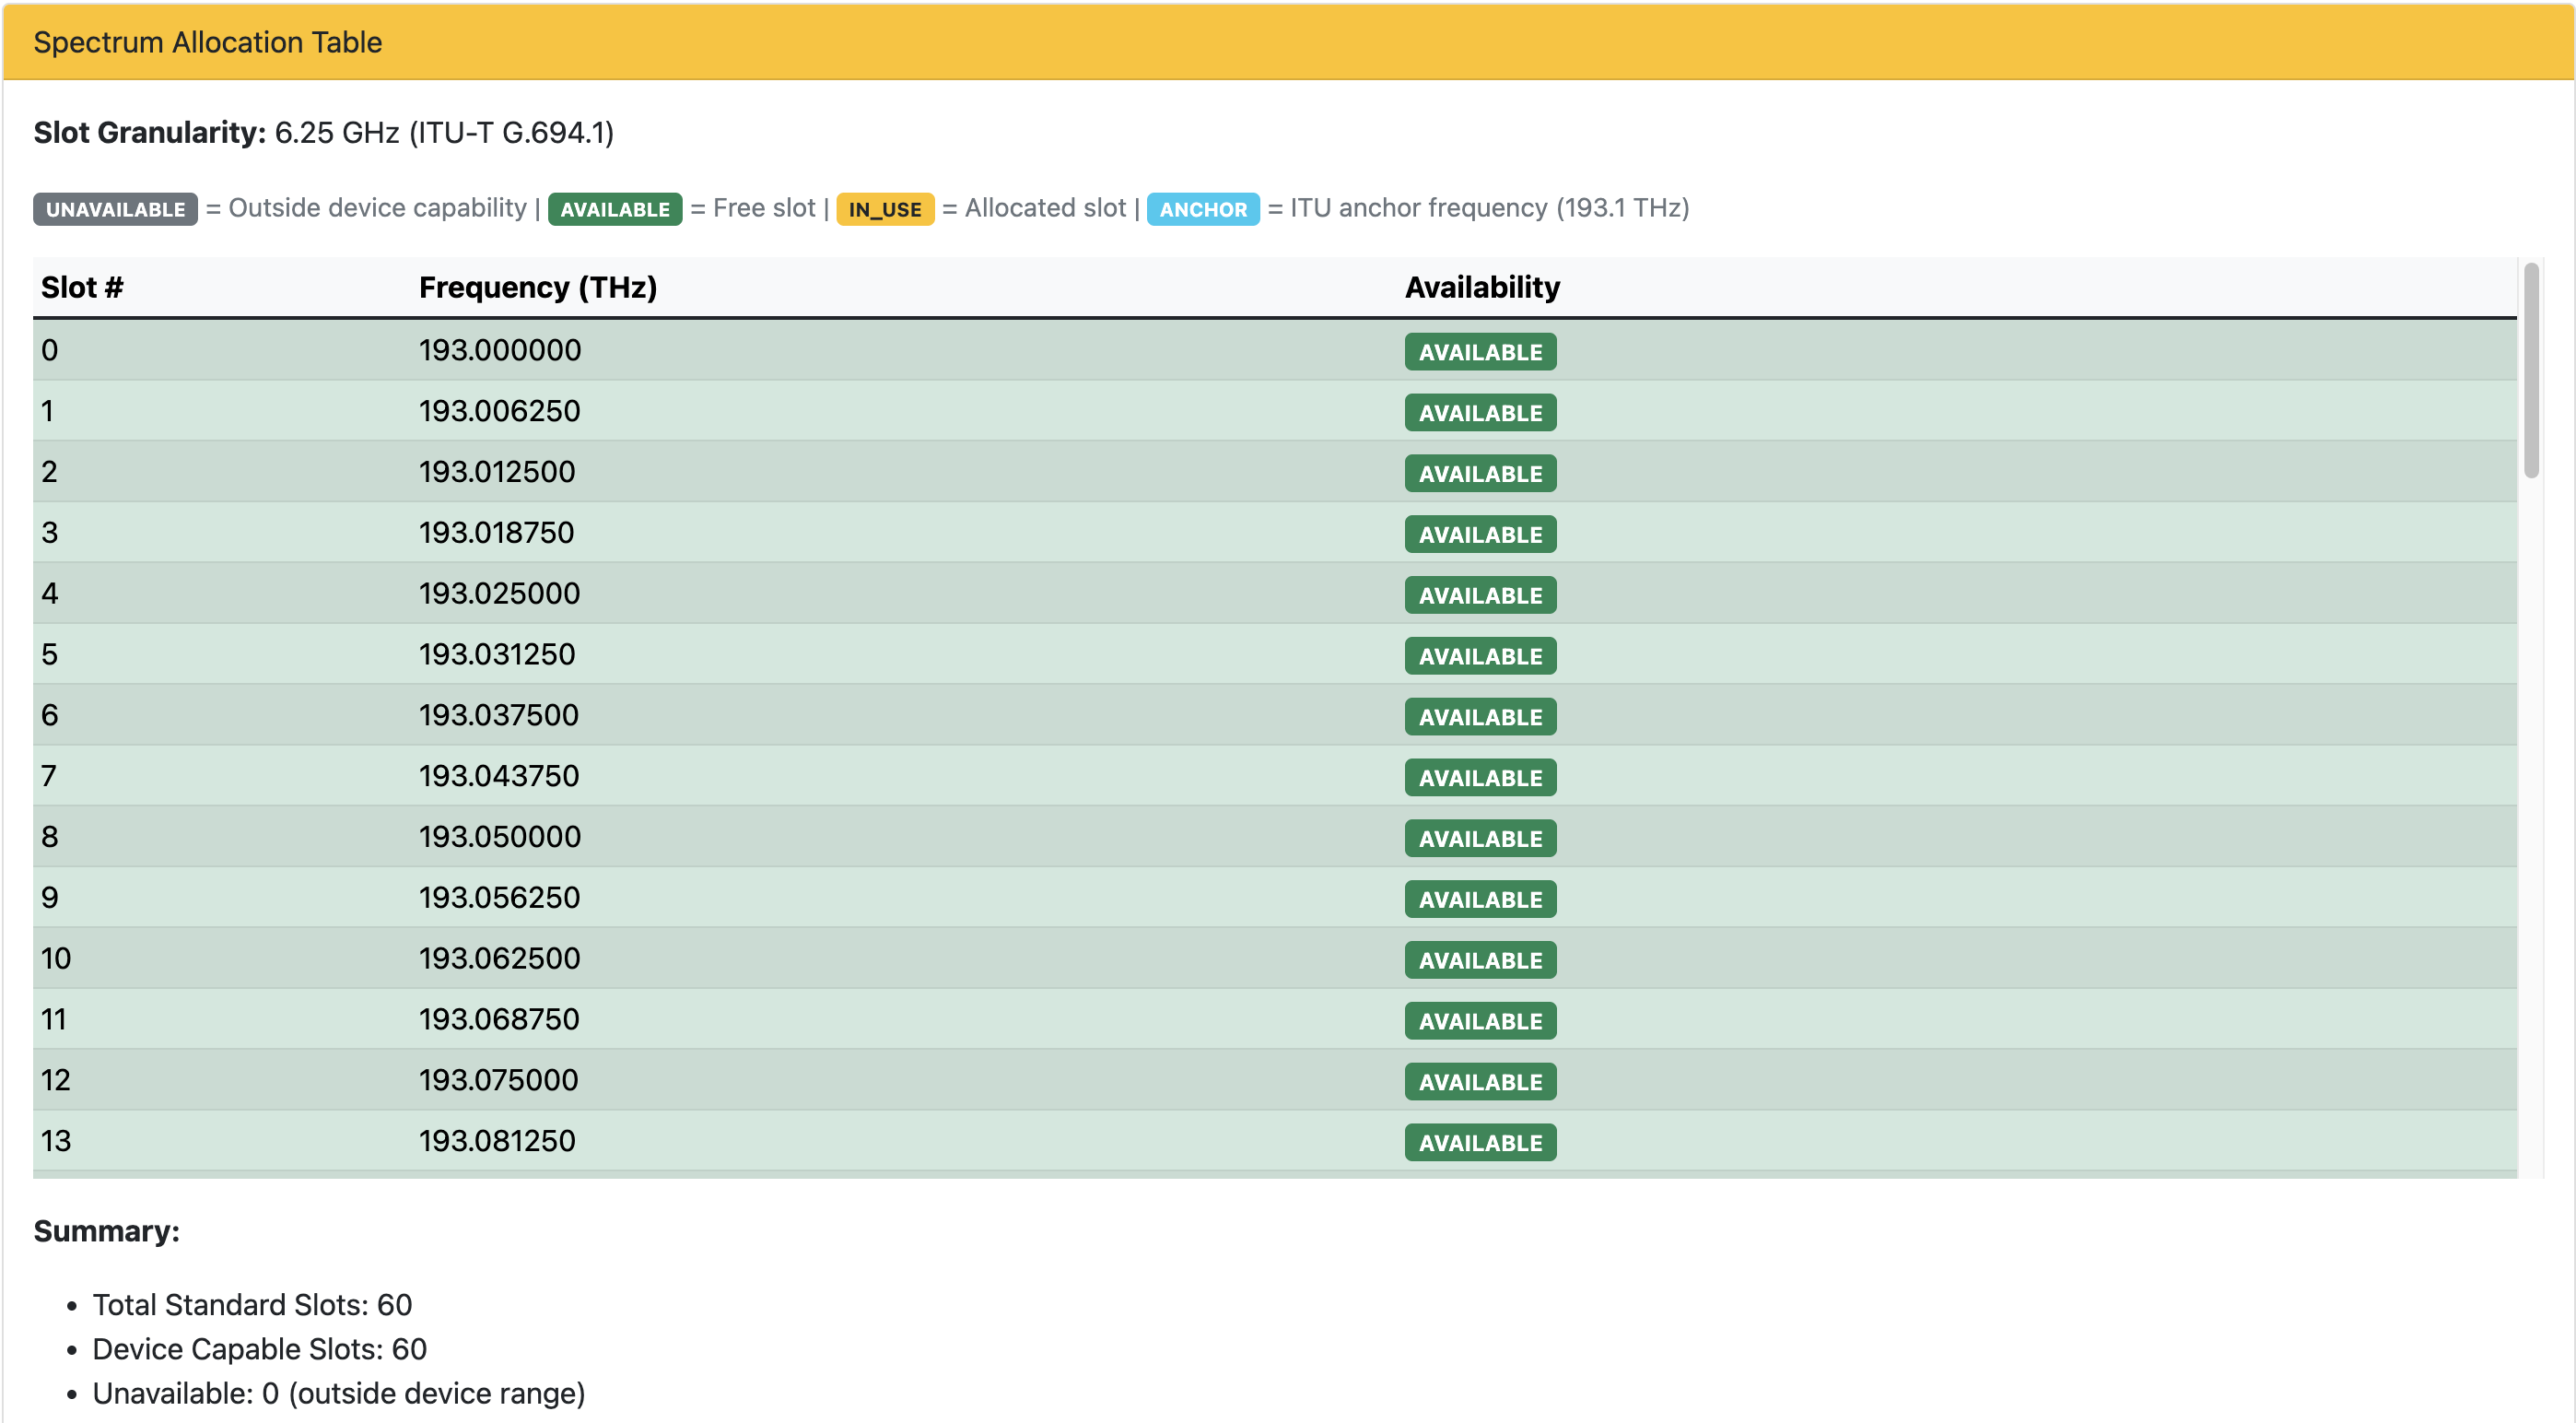
\includegraphics[width=0.8\textwidth]{port_rsa.png}
    \caption{Frequency details of an Endpoint}
    \label{fig:port_rsa}
\end{figure}
\subsection*{\small Link RSA Comparison}
This section validates the effectiveness of the ParallelOpticalController's RSA algorithm by presenting a direct visual comparison of link spectrum utilization before and after the allocation of a lightpath request. In a multi-fiber network, managing frequency continuity across parallel physical links is computationally challenging. The proposed bitmap-based approach addresses this by dynamically evaluating all available spatial dimensions simultaneously to identify suitable, contiguous spectrum gaps.
\begin{figure}[htbp]
    \centering
    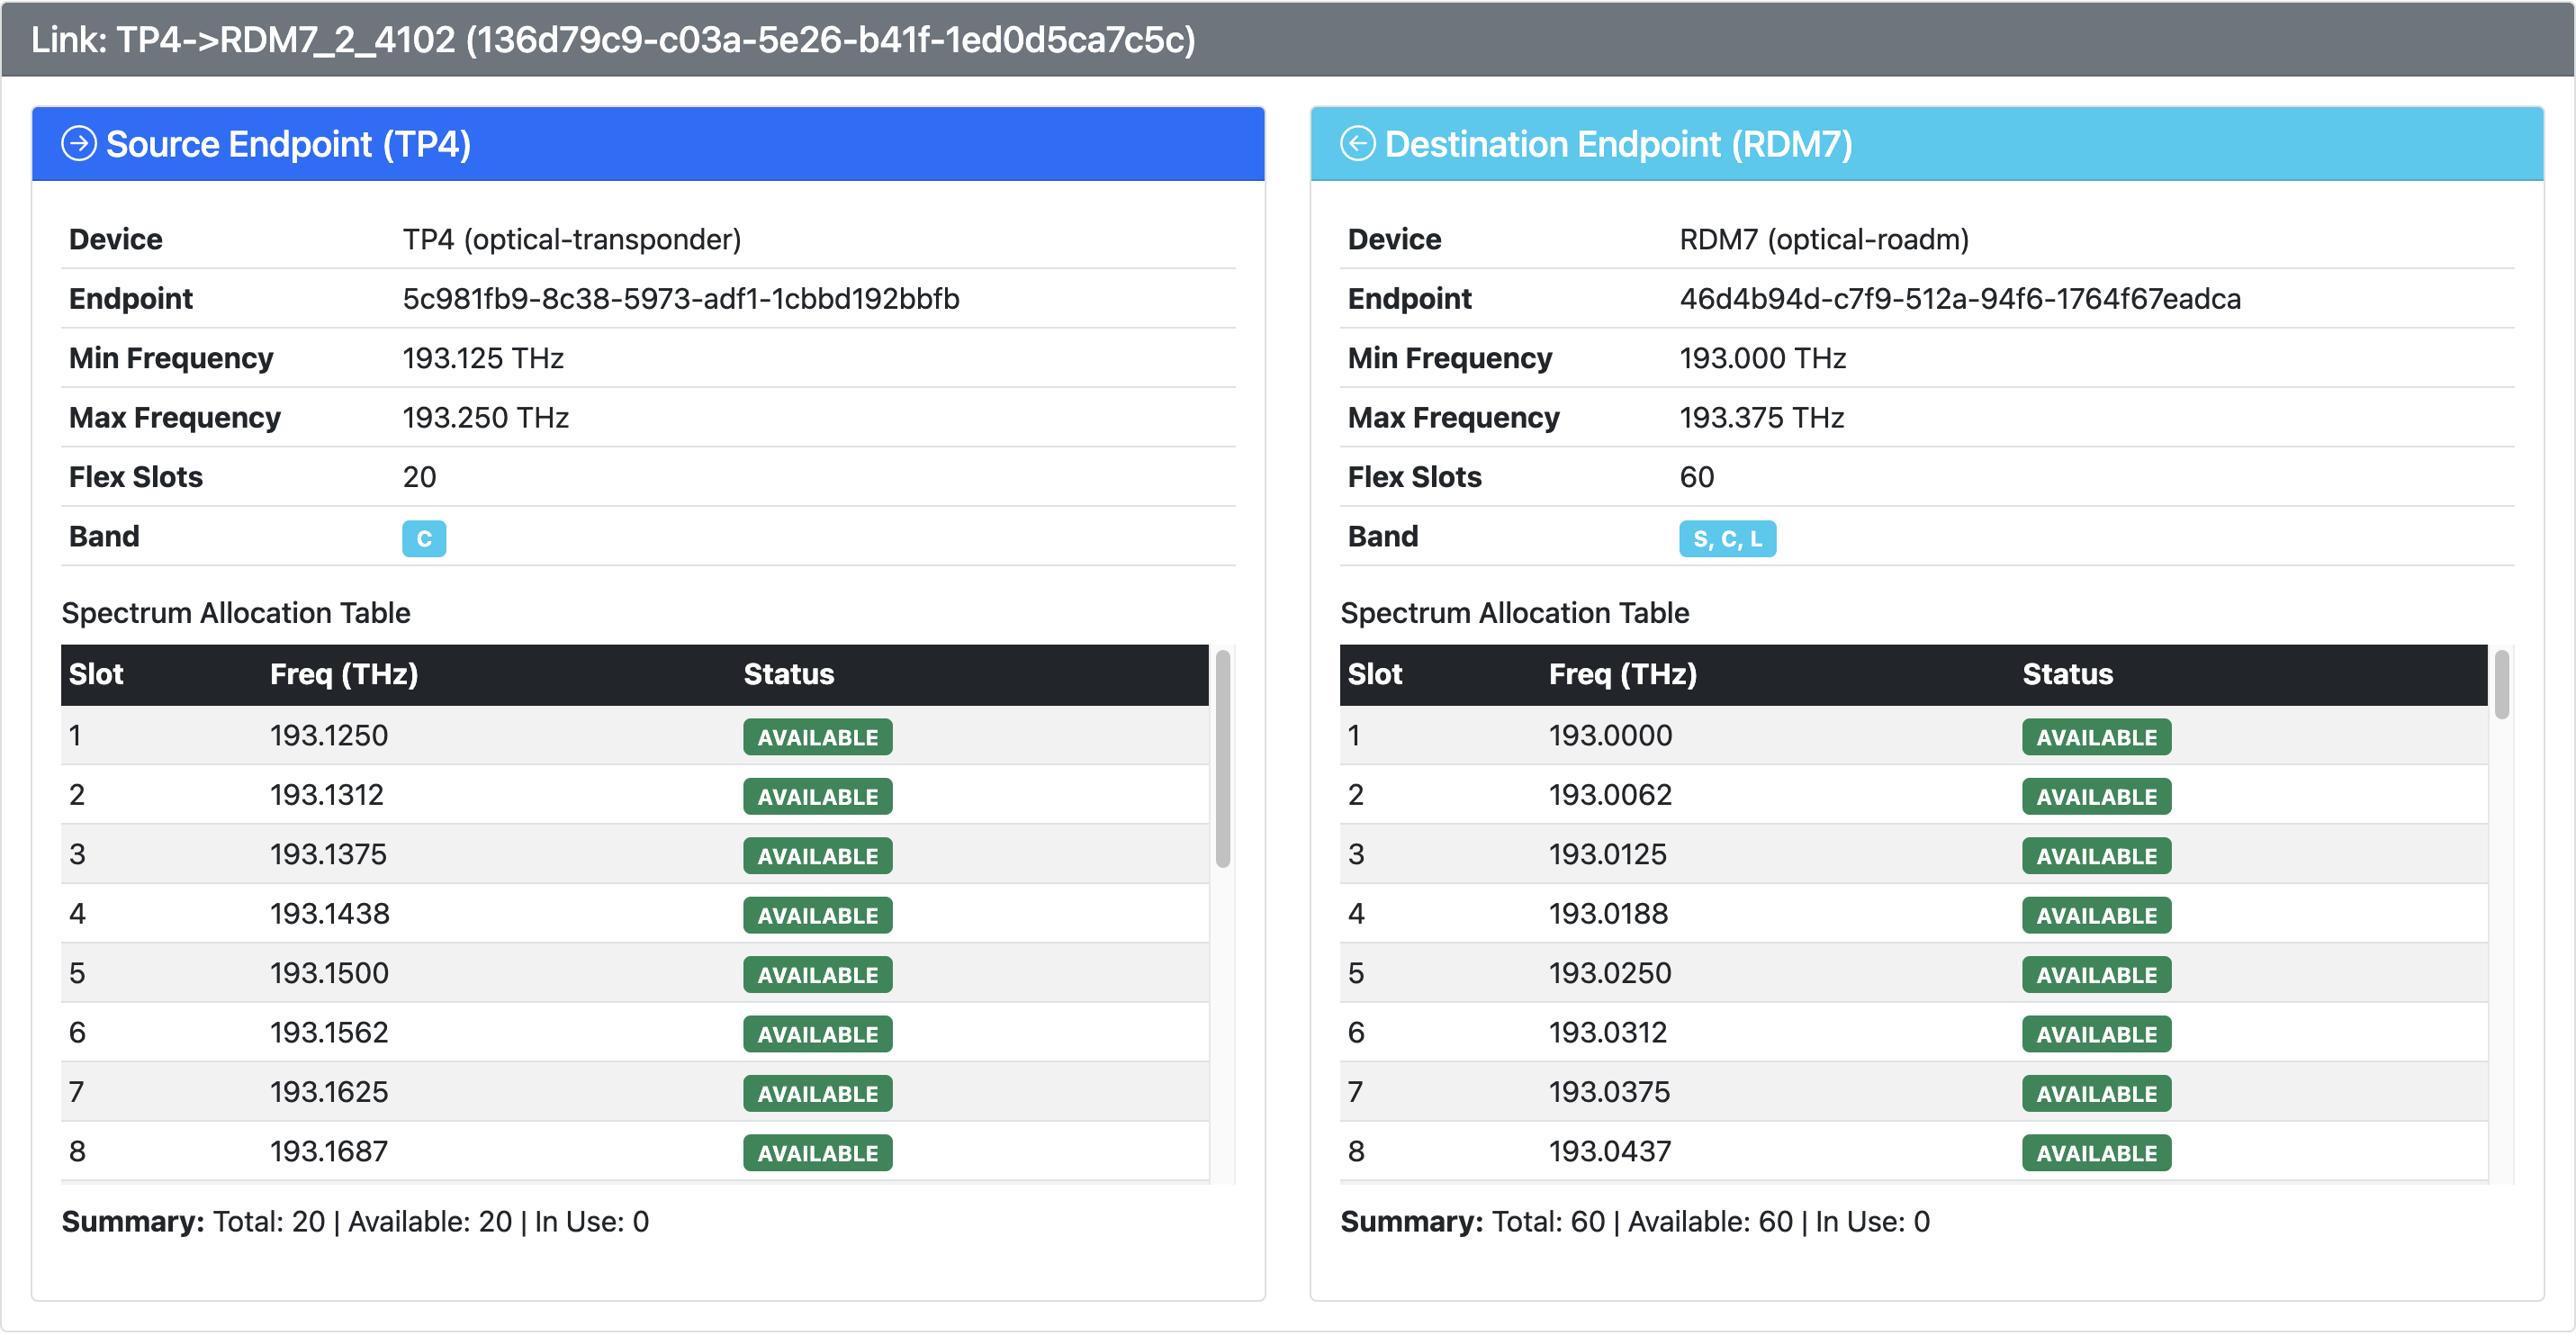
\includegraphics[width=0.8\textwidth]{link_rsa.png}
    \caption{DWDM flex-grid details of Link}
    \label{fig:link_rsa}
\end{figure}
\subsection*{\small RSA Computation of a Lightpath}
The Routing and Spectrum Allocation (RSA) phase represents the core operational logic of the ParallelOpticalController. This section validates the algorithmic execution by tracing a specific lightpath request from initiation to final spectral assignment. The functional validation focuses on the transition from topological path discovery to the bitwise spatial-spectral intersection. As demonstrated in the following images, the controller first identifies the primary shortest path using Dijkstra's algorithm on the simplified graph $(G_simple)$. Following path discovery, the controller executes a hop-by-hop analysis of the spectral state. For every hop, the controller retrieves the occupancy bitmaps of all constituent parallel links and performs a concurrent bitwise intersection. This process collapses the spatial complexity of the multi-fiber bundle into a single, unified availability bitmap, ensuring that the selected contiguous slots are physically available across the entire spatial breadth of the link.
\begin{figure}[htbp]
    \centering
    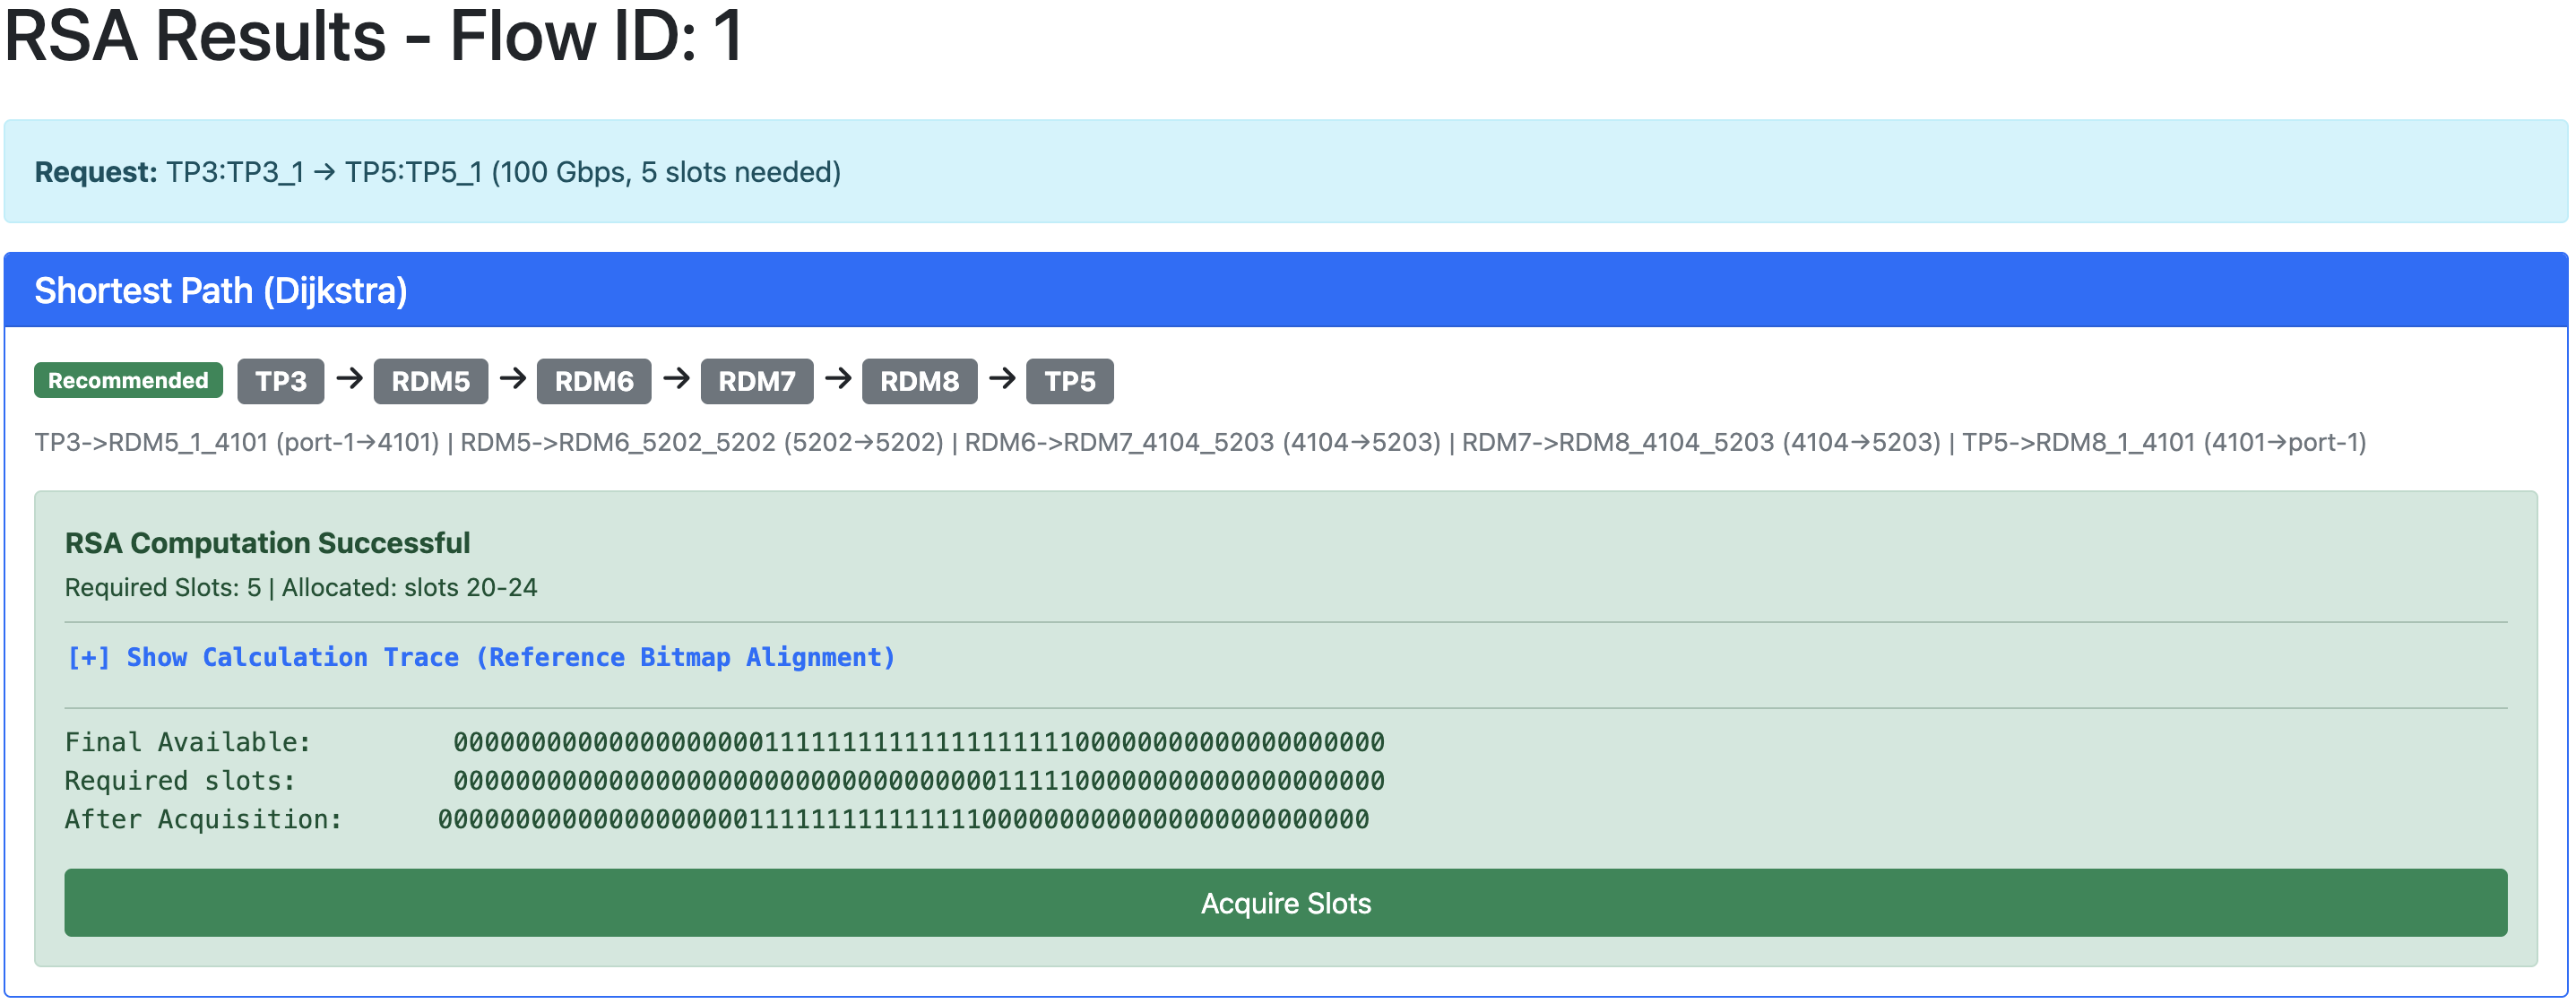
\includegraphics[width=0.8\textwidth]{shortest_path.png}
    \caption{Shortest path discovery}
    \label{fig:shortest_path}
\end{figure}
\begin{figure}[htbp]
    \centering
    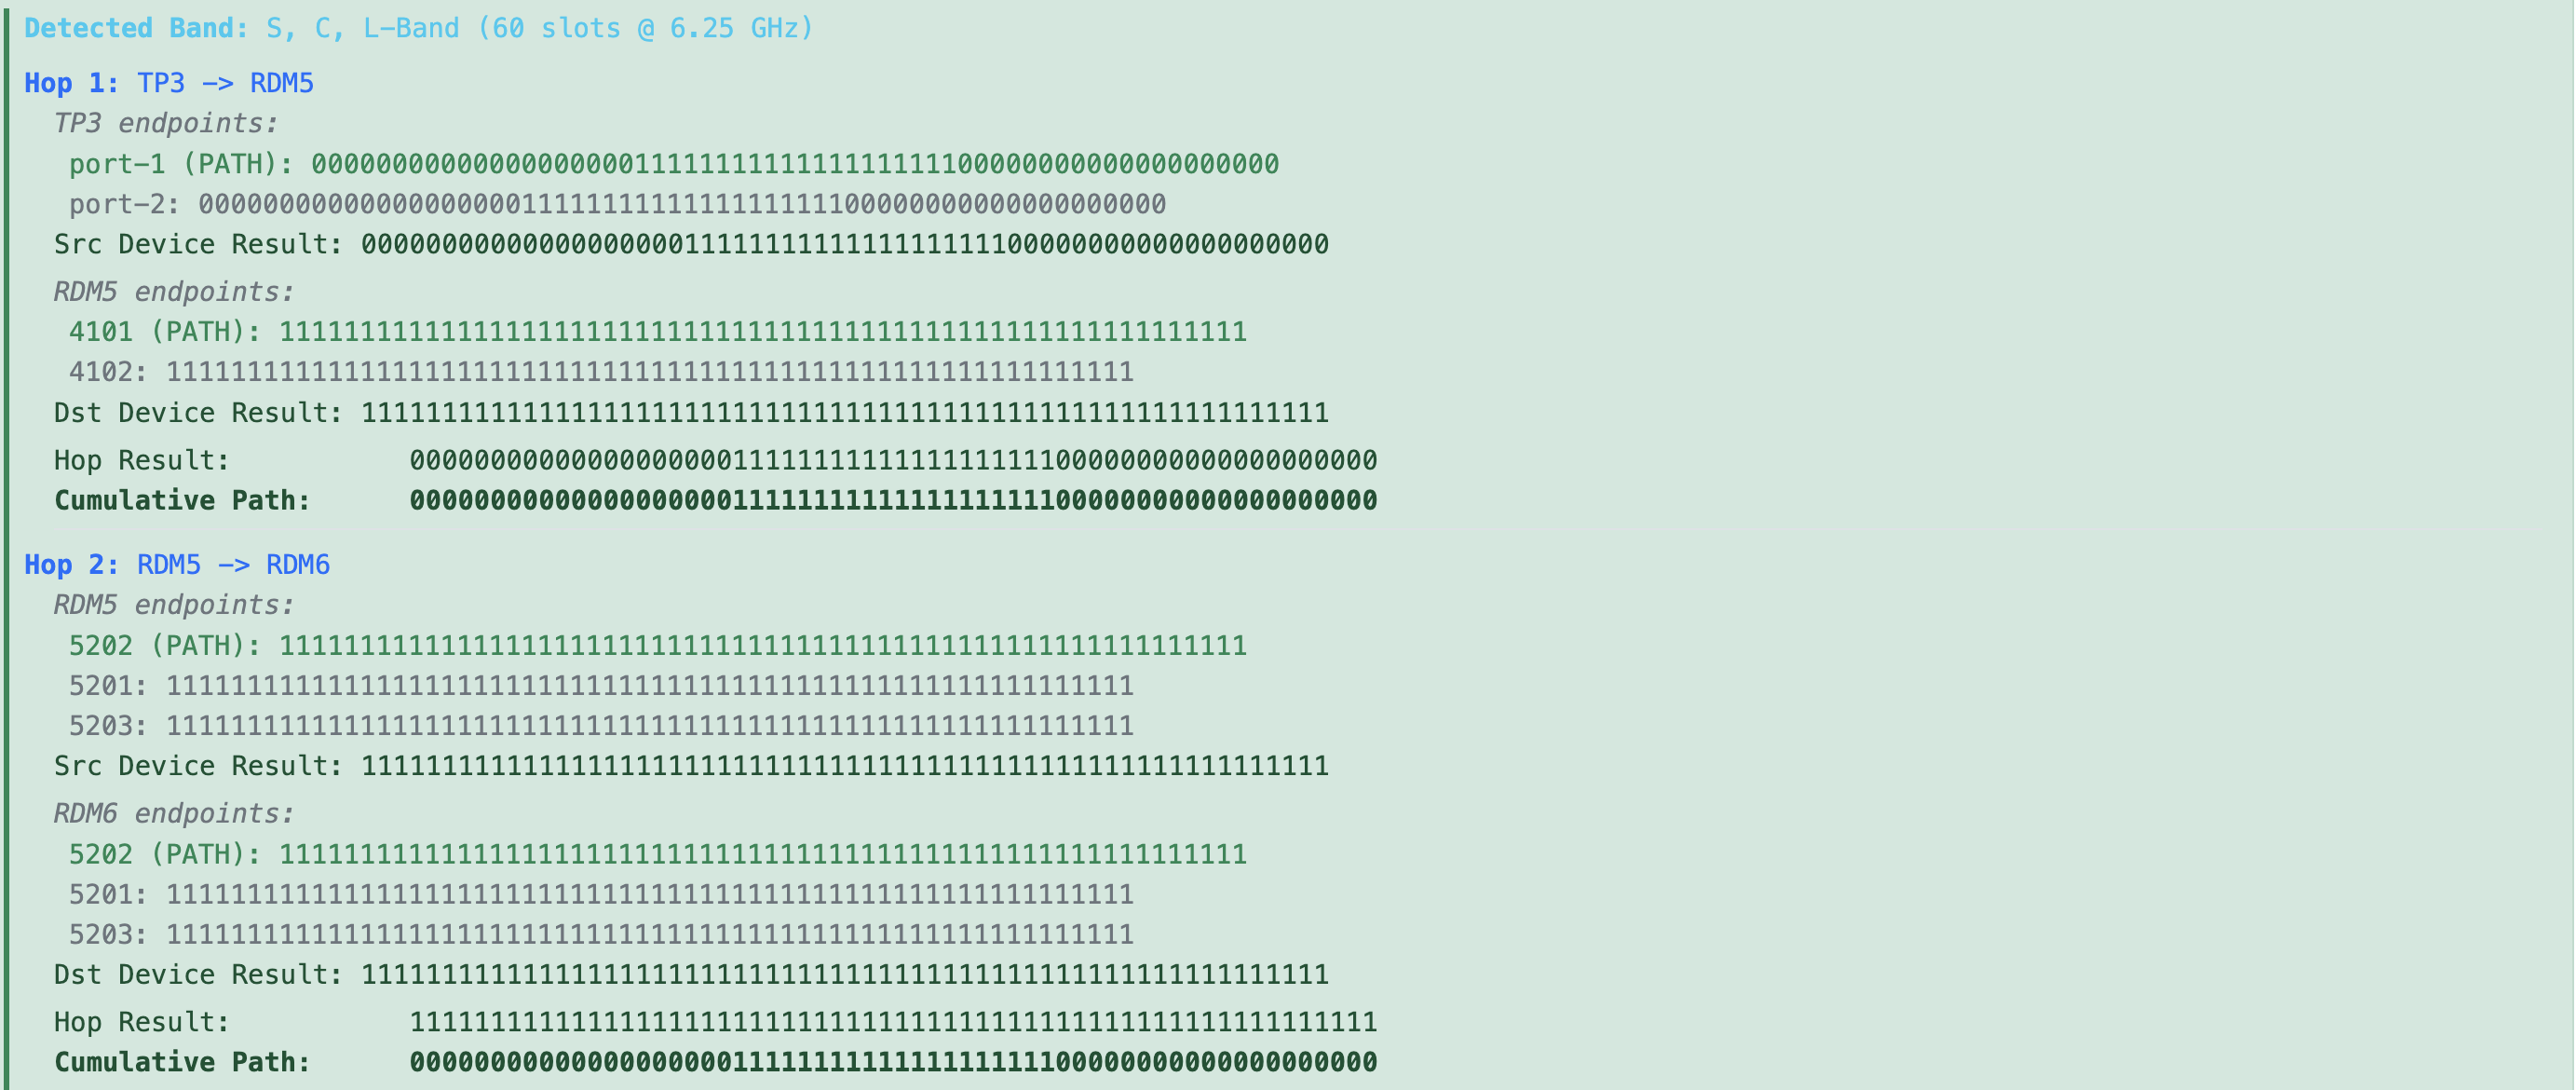
\includegraphics[width=0.8\textwidth]{hop_rsa.png}
    \caption{Hop-by-hop RSA computation}
    \label{fig:hop_rsa}
\end{figure}

\begin{figure}[htbp]
    \centering
    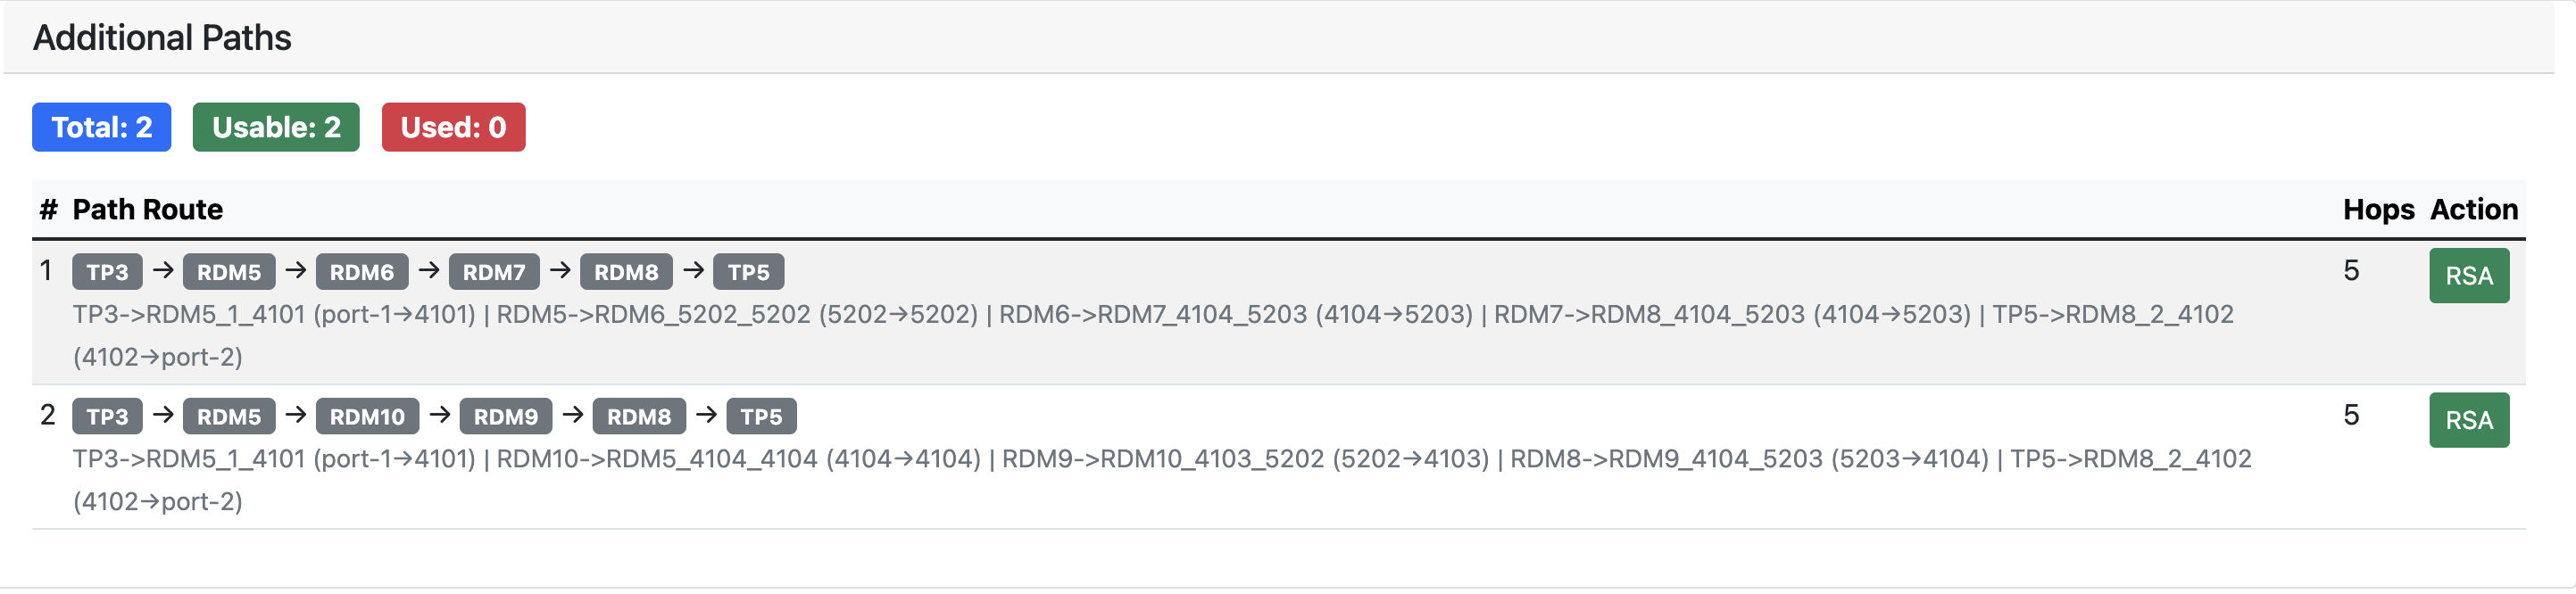
\includegraphics[width=0.8\textwidth]{additional_path.png}
    \caption{Additional Path Computation}
    \label{fig:additional_path}
\end{figure}
\section{Performance Evaluation \& Efficiency Analysis}
This section provides a quantitative analysis of the computational latency introduced by the ParallelOpticalController during the provisioning lifecycle. To assess the scalability and algorithmic efficiency of the controller, execution times were recorded across four distinct sequential phases: Graph Generation, Shortest Path Computation, RSA Computation, and Additional Path Computation. Measurements were taken across the four reference topologies (Linear, Butterfly, NSF, and PANEU), with each evaluated in both a standard single-fiber baseline and a highly dense multi-fiber parallel configuration. All execution metrics are measured in seconds.
\begin{table}[htbp]
    \centering
    \resizebox{\textwidth}{!}{\begin{tabular}{|c|c|c|c|c|c|}
            \hline
            \textbf{Topology}  & \textbf{Graph gen.} & \textbf{Shortest path com.} & \textbf{RSA comp.} & \textbf{Additional path comp.} & \textbf{Efficiency} \\
            \hline
            Linear Single      & 0.0018              & 0.0012                      & 0.0003             & 0.0009                         & -                   \\
            \hline
            Linear Parallel    & 0.0018              & 0.0016                      & 0.0005             & 0.0009                         & 87.50\%             \\
            \hline
            Butterfly Single   & 0.0014              & 0.0008                      & 0.0004             & 0.0007                         & -                   \\
            \hline
            Butterfly Parallel & 0.0017              & 0.0016                      & 0.0007             & 0.0007                         & 70.21\%             \\
            \hline
            NSF Single         & 0.0019              & 0.0016                      & 0.0007             & 0.0023                         & -                   \\
            \hline
            NSF Parallel       & 0.0022              & 0.0021                      & 0.0011             & 0.0024                         & 83.33\%             \\
            \hline
            PANEU Single       & 0.0024              & 0.0024                      & 0.0013             & 0.0134                         & -                   \\
            \hline
            PANEU Parallel     & 0.0026              & 0.0027                      & 0.0019             & 0.0141                         & 91.54\%             \\
            \hline
        \end{tabular}}
    \caption{Efficiency evaluation of ParallelOpticalController}
    \label{tab:complexity_analysis_table}
\end{table}

\subsection*{\small Phase Analysis and Scalability}
\begin{enumerate}
    \item \textbf{Graph Abstraction and Path Discovery} \vspace{0.2cm}\\
          As established in the theoretical complexity analysis, the graph generation phase operates in linear time. The empirical data strongly corroborates this; graph generation latency scales predictably with network size, ranging from a mere 0.0018 seconds in the minimalist Linear topology to $0.0026$ seconds in the heavily meshed PANEU Parallel topology. Similarly, the Shortest Path Computation time remains highly constrained. Because the controller intelligently collapses parallel physical links into a unified logical graph $(G_{simple})$ prior to routing, Dijkstra's algorithm avoids traversing redundant parallel edges. Consequently, the path computation time for the massive PANEU Parallel network requires only $0.0027$ seconds—a negligible $0.0003$-second increase over its single-fiber counterpart.
    \item \textbf{Routing and Spectrum Allocation (RSA) Execution} \vspace{0.2cm}\\
          The RSA Computation phase serves as the most critical benchmark for the proposed algorithm. Traditional sequential allocation methods suffer from exponential state-space explosion when parallel links are introduced. In stark contrast, the empirical data demonstrates that the controller's spatial bitwise intersection completely bypasses this bottleneck.

          Across all evaluated topologies, the RSA computation executed in fractions of a millisecond. For instance, transitioning from the NSF Single to the NSF Parallel configuration only increased the RSA computational overhead from $0.0007$ seconds to $0.0011$ seconds. Even under the extreme spatial complexity of the PANEU Parallel topology, the RSA computation was finalized in just $0.0019$ seconds. This confirms the mathematical claim that the spatial bitwise operation natively evaluates parallel link bundles concurrently, reducing an exponentially complex problem to a highly efficient linear evaluation.
\end{enumerate}
\subsection*{\small Overall Algorithmic Efficiency}
To formalize the comparative performance between single-fiber and multi-fiber operations, an Efficiency metric was calculated for each parallel topology using the following ratio of total computation times:
\[
    \varepsilon=\frac{Time_{single-link}}{Time_{parallel-link}}\times 100
\]
This metric illustrates the latency penalty incurred by introducing parallel routing constraints. An efficiency score closer to $100\%$ indicates that the parallel architecture processes requests almost as rapidly as a simplified single-fiber network. The results demonstrate outstanding operational resilience. The Linear and NSF Parallel topologies maintained high efficiencies of $87.50\%$ and $83.33\%$, respectively. The Butterfly Parallel topology, due to its specific highly-meshed parallel interconnections relative to its small node count, yielded a slightly lower efficiency of $70.21\%$. Most notably, the largest and most complex network evaluated—the PANEU Parallel topology—achieved the highest efficiency rating of $91.54\%$.

Ultimately, these metrics definitively prove that the \texttt{ParallelOpticalController} successfully mitigates the heavy computational burdens typically associated with multi-fiber elastic optical networks. By processing complex, parallel spatial-spectral allocations in under two milliseconds, the controller guarantees real-time provisioning capabilities regardless of underlying physical fiber density.
\section{Throughput Analysis}
While the preceding section analyzed the isolated computational latency of individual algorithmic phases, this section evaluates the aggregate operational capacity of the \texttt{ParallelOpticalController}. In the context of the Software-Defined Networking (SDN) control plane, throughput is critical for evaluating the controller's viability in highly dynamic, real-world network environments where connection requests arrive continuously and require immediate resolution. Within the SDN control plane, throughput is fundamentally defined as the maximum sustainable rate of lightpath provisioning requests the controller can successfully process per unit of time. To mathematically derive this metric, it is first necessary to establish the total computational time, denoted as $T_{\text{total}}$, required to process a single, end-to-end request. This aggregate time variable encapsulates the sum of the latencies incurred across all distinct execution phases: the initial graph abstraction, shortest path discovery, the core spatial-spectral RSA computation, and any requisite alternative path calculations. Once the aggregate processing latency is established, the control plane \texttt{throughput}, represented by the variable $\lambda$, can be determined through an inverse proportional relationship to the total processing time. Specifically, the throughput is calculated using the following mathematical formulation:
\[
    \lambda=\frac{1}{T_{\text{total}}} \text{ (requests/second)}
\]
By applying this formula to the empirical latency metrics recorded in the preceding section, the aggregate processing capacity of the \texttt{ParallelOpticalController} can be accurately quantified across the evaluated spectrum of topological complexities.

In the smaller, less complex architectures, the controller exhibited exceptional throughput. For the baseline Linear Single topology, the controller processed requests at a rate of approximately 238 requests per second. When scaling up to the multi-fiber Linear Parallel configuration, throughput remained highly robust at 208 requests per second. Similarly, in the mid-scale NSFNet topology—which serves as a highly representative model for standard wide-area networks—the controller maintained a throughput of 153 requests per second in the single-fiber configuration. When subjected to the dense spatial requirements of the NSF Parallel configuration, the system successfully resolved 128 requests per second. This demonstrates that introducing the massive physical capacity of parallel fibers only marginally diminishes the controller's processing rate, validating the efficiency of the bitwise spatial intersection algorithm.

As topological complexity approaches the extreme scale of the Pan-European (PANEU) network, a natural reduction in control plane throughput is observed due to the sheer volume of nodes and interconnected edges. The PANEU Single topology yielded a throughput of approximately 51 requests per second. However, even when operating within the PANEU Parallel environment—the most computationally demanding scenario evaluated, featuring 37 nodes and 105 parallel links—the \texttt{ParallelOpticalController} sustained a stable throughput of 46 requests per second.
\section{Statistical Analysis}
\textbf{TBD: (This section requires a deeper mathematical and statistical evaluation of the results. I will provide an analysis of the blocking paths and theoretical channel capacity against the actual used capacity during peak simulation periods.)}
\chapter{Conclusion and Future Work}
This concluding chapter summarizes the overarching achievements and technical contributions presented throughout this thesis. It critically reflects on the practical constraints and structural limitations encountered during the implementation phase and outlines potential avenues for future research to further refine the management of flexible-grid optical networks within TeraFlowSDN.
\section{Summary of Contributions}
This thesis presented a comprehensive integration of a parallel-link-supported Routing and Spectrum Allocation (RSA) framework within the TeraFlowSDN (TFS) ecosystem. The core objective of managing parallel optical links and enhancing physical layer visibility was achieved through targeted architectural, algorithmic, and interface-level developments. The primary contributions of this research are summarized as follows:
\begin{itemize}
    \item \textbf{Enhancement of Device Drivers:} Substantial modifications were implemented within the OpenConfig \texttt{(OCDriver)} and OpenROADM drivers to extract foundational device metadata, including hardware versions, software versions, and manufacturer nomenclature. The parsing mechanisms were fundamentally overhauled using a two-phase extraction process and model-based filtering, allowing the controller to dynamically compute and store critical RSA parameters—such as minimum/maximum frequencies and flex grid slots—directly into an extended Context Service database schema.
    \item \textbf{ParallelOpticalController and RSA Implementation:}\\ \texttt{ParallelOpticalController} microservice was developed and deployed as a core component of the TFS ecosystem to manage complex optical intents. By leveraging NetworkX to construct multi-directed graphs, the architecture successfully modeled multi-edge parallel optical links. The path computation engine utilized a stateful, bitmap-based intersection methodology adhering to the ITU-T G.694.1 6.25 GHz slot granularity to accurately discover, compute, and allocate contiguous spectrum spaces across varying topologies.
    \item \textbf{UI and UX Enhancements:} The default TFS WebUI was significantly augmented to provide comprehensive spectrum visualization. A dynamic Spectrum Allocation Table was introduced to display explicit slot availability (categorized as \texttt{AVAILABLE}, \texttt{UNAVAILABLE} and \texttt{IN\_USE}) derived directly from endpoint frequency capabilities. Furthermore, parallel links were visually abstracted using a numeric notation within the topology viewer, ensuring clear topological representation without graphical overflow.
\end{itemize}
Collectively, these structural and algorithmic enhancements facilitated a highly responsive and deterministic optical control plane. The computational performance and spectrum utilization efficiency evaluations demonstrated that the bitmap-based allocation algorithm efficiently handles heavy topological data while minimizing spectrum fragmentation. Furthermore, the throughput analysis—validated through rigorous testing of network-level traffic loads—confirmed that the system maintains an optimal blocking probability by dynamically distributing slot allocations across all available parallel links. While the proposed solutions achieved strict functional validation and showcased strong computational efficiency, the development and physical testbed deployment phases surfaced specific architectural and environmental constraints. These systemic boundaries define the operational envelope of the current controller architecture and introduce several critical limitations that must be addressed.
\section{Limitations}
While the integration of the \texttt{ParallelOpticalController} introduces significant capabilities to the TeraFlowSDN (TFS) ecosystem—particularly in managing parallel optical links and rendering detailed spectrum visualizations—the current framework inherently operates within specific systemic and architectural boundaries. Acknowledging these limitations is critical for understanding the operational envelope of the proposed solution and identifying areas for continuous research. The constraints can be broadly categorized into architectural dependencies, algorithmic assumptions, and device-level interactions.
\subsection*{\small Architectural Dependencies and Performance Overheads}
A fundamental architectural limitation is the stateful operation of the \texttt{ParallelOptic-\\alController}. By design, microservices are traditionally engineered to be stateless and independently executable. However, the proposed RSA computation engine is deeply ingrained within the TFS control plane, heavily relying on continuous synchronization with the Context Service to fetch the latest topology, optical configurations, and device capabilities. While statefulness is a common paradigm in centralized Software-Defined Networking (SDN) architectures, it tightly couples the controller to the TFS database schema, limiting its standalone portability. Furthermore, this state dependency introduces significant performance overheads. The current implementation relies on a quantitative volume of database queries to extract granular endpoint indexes, associated channel mappings, and flex-grid bitmap values across the multi-directed graph. This iterative polling of the database during the \texttt{find\_paths()} and \texttt{expand\_path()} execution phases introduces computational latency. In highly scaled networks with dense parallel links, this latency could scale linearly, potentially impacting real-time provisioning SLA requirements.

\subsection*{\small Algorithmic and Topological Assumptions}
The algorithmic approach to graph modeling and path discovery introduces several operational constraints. First, the \texttt{NetworkX} graph construction \texttt{(G\_FREE and G\_simple\_free)} fundamentally assumes that all optical links are bi-directional. The Dijkstra-based shortest path and simple path expansion algorithms compute routing metrics based on this symmetry. If the physical infrastructure contains uni-directional optical fibers or asymmetric spectrum availability, the current algorithmic formulation will fail to discover a valid end-to-end lightpath. Second, there is a topological abstraction limitation regarding ROADM internal architectures. The graph expansion mechanism assumes that any parallel links connecting a Transponder to a ROADM, or between two ROADMs, are functionally equivalent as long as they reach the target node. However, it currently does not account for the specific spatial Degrees (DEGs) to which these fibers terminate. As observed in the roadm.xml definitions (e.g., ports designated to D1 versus D2), if a fiber terminates on a different DEG, the internal optical cross-connect (OXC) constraints of the ROADM might prevent successful switching. The controller currently abstracts this away, treating any parallel link to the same device as a valid routing option, which could lead to physically unrealizable path computations.

\subsection*{\small Lifecycle Management and Device-Level Interactions}
From an operational lifecycle perspective, the current framework focuses primarily on the establishment of optical intents. The slot acquisition process currently requires manual intervention and intuitive oversight by the network operator. More importantly, the controller does not natively support an automated lightpath teardown and slot release mechanism. Once slots are marked as \texttt{IN\_USE} in the spectrum bitmap, reversing this hash to free the contiguous 6.25 GHz slots upon intent deletion requires manual reconciliation. Finally, the device interaction layer remains bounded by the scope of the testbed. The enhanced information extraction mechanisms within OCDriver and OpenROADMDriver (utilizing filtering modules and targeted model-based extraction) were engineered and validated against specific emulated environments (e.g., SSSA-CNIT Mellanox emulators and virtual ROADMs). This means the extraction logic is heavily tailored to these configurations. A wider array of device configurations and vendor-specific YANG models must be studied to provide generalized, built-in support for diverse physical hardware. Because the controller has not yet been validated against real, physical transponders and ROADMs in a hardware testbed, unforeseen hardware idiosyncrasies, netconf session timeouts, or proprietary XML formatting could introduce unknown errors. Additionally, while the RSA algorithm successfully computes the path and updates the logical SDN database, it lacks the southbound provisioning logic to actively push the required cross-connect configurations down to the physical devices' local databases. Currently, the solution remains fully analytical and logical within the SDN control plane.
\section{Future Work Directions}
Building upon the established framework and the identified limitations, several highly promising avenues for future research and development emerge. The transition from a logical, stateful microservice to an autonomous, hardware-validated optical controller requires focusing on the following key areas:
\subsection*{\small Vendor-Agnostic Device Abstraction and Hardware Validation}
Transitioning the current framework from emulated environments to physical hardware testbeds is a paramount next step. Future iterations of this research should expand the OCDriver and OpenROADMDriver to encompass a broader array of commercial vendor equipment (e.g., Cisco, Nokia, Ciena) and their respective, complex YANG data models. By building a generalized, vendor-agnostic device abstraction layer, the controller can seamlessly adapt to diverse hardware idiosyncrasies. Furthermore, the framework must be extended to include active southbound provisioning. Rather than merely updating the logical state within the TeraFlowSDN database, future work must focus on actively pushing the computed optical cross-connects and frequency configurations directly to the physical network elements via NETCONF.
\subsection*{\small Algorithmic Refinement for Spatial and Directional Constraints}
To accurately reflect the physical realities of modern transport networks, the RSA algorithm must be decoupled from its assumption of strict bi-directionality. Future work should enhance the \texttt{NetworkX} graph modeling to natively support uni-directional optical fibers and asymmetric spectrum bands. Crucially, the path discovery and expansion algorithms must be upgraded to comprehend ROADM internal architectures. Incorporating node-internal spatial constraints—specifically validating that parallel fibers terminating on different spatial Degrees (DEGs) can establish a valid cross-connect—will ensure that computed lightpaths are physically viable at the photonics level.
\subsection*{\small Automated Lifecycle and Spectrum Management}
To achieve a fully autonomous, intent-based network ecosystem, the controller must evolve to manage the complete lifecycle of an optical intent. Research must be directed toward fully automating the slot acquisition process, removing the need for manual operator intervention. More importantly, dynamic lightpath teardown and slot release mechanisms must be implemented. Developing algorithms to intelligently reverse the spectrum bitmap hashes, automatically freeing and coalescing contiguous 6.25 GHz slots upon intent deletion, will be critical for preventing spectrum fragmentation over time.
\subsection*{\small Architectural Optimization for Low-Latency Computation}
To mitigate the latency introduced by the high volume of sequential database queries during the graph expansion and RSA computation phases, the controller's architecture requires optimization. Future research should investigate the integration of an in-memory, distributed caching layer (such as Redis) directly accessible by the ParallelOpticalController. By caching the topological state, device capabilities, and current spectrum bitmaps, the computation engine can reduce its strict dependence on the centralized Context Service. This architectural shift would drive the microservice closer to a stateless operational paradigm, significantly reducing path computation times and improving overall scalability in dense, highly parallelized network topologies.

In conclusion, this thesis successfully bridges a critical gap in the TeraFlowSDN ecosystem by introducing robust support for parallel optical links and granular spectrum management. Through the development of the Parallel Optical Controller microservice and the targeted enhancement of device-level data extraction, the research demonstrates a highly capable approach to Routing and Spectrum Allocation (RSA) within a modern software-defined architecture. While specific architectural dependencies, algorithmic assumptions, and the need for physical hardware validation delineate the boundaries of the current framework, the foundation laid by this work provides a vital stepping stone for continuous development. Ultimately, these structural and algorithmic contributions significantly advance the capacity of SDN controllers to visualize, compute, and orchestrate complex, next-generation optical transport networks with enhanced precision and reliability.
\end{document}